\documentclass[11pt,oneside,openany]{book}
\newcommand{\ShortTitle}{HODGE / CYCLES AND CONSTRUCTORS}
\usepackage[T1]{fontenc}
\usepackage[utf8]{inputenc}
\usepackage{mathpazo}
\usepackage[scaled=0.92]{helvet}
\usepackage{courier}
\usepackage{amsmath,amssymb,amsthm,mathtools}
\usepackage[a4paper,left=27mm,right=27mm,top=26mm,bottom=27mm,headheight=15pt]{geometry}
\usepackage{microtype}
\usepackage{graphicx}
\usepackage[dvipsnames]{xcolor}
\usepackage{booktabs,array,longtable,tabularx}
\usepackage{enumitem}
\usepackage{titlesec,fancyhdr}
\usepackage{caption}
\usepackage{hyperref}
\definecolor{Ink}{HTML}{243138}
\definecolor{Teal}{HTML}{21676B}
\definecolor{Copper}{HTML}{A45C36}
\definecolor{Soft}{HTML}{E9F0EF}
\definecolor{Gray}{HTML}{627078}
\hypersetup{colorlinks=true,linkcolor=Teal,citecolor=Teal,urlcolor=Teal,pdfauthor={Komorebi P.}}
\urlstyle{same}
\setlength{\parindent}{1.2em}
\setlength{\parskip}{0.15em}
\linespread{1.09}
\setlist{itemsep=0.22em,topsep=0.45em,leftmargin=1.55em}
\setlist[description]{style=nextline,leftmargin=0pt,labelwidth=0pt,labelsep=0pt,font=\normalfont\bfseries}
\setcounter{tocdepth}{2}
\setlength{\emergencystretch}{1.4em}
\titleformat{\section}{\Large\bfseries\color{Ink}}{\thesection}{0.7em}{}
\titleformat{\subsection}{\large\bfseries\color{Ink}}{\thesubsection}{0.7em}{}
\titleformat{\subsubsection}{\normalsize\bfseries\color{Ink}}{\thesubsubsection}{0.7em}{}
\titlespacing*{\section}{0pt}{1.8em}{0.7em}
\titlespacing*{\subsection}{0pt}{1.3em}{0.5em}
\captionsetup{font=small,labelfont={bf,color=Teal},skip=8pt}
\pagestyle{fancy}
\fancyhf{}
\fancyhead[L]{\sffamily\scriptsize\color{Gray}OPERATION KOMOREBI}
\fancyhead[R]{\sffamily\scriptsize\color{Gray}\ShortTitle}
\fancyfoot[L]{\sffamily\scriptsize\color{Gray}CONJECTURE SERIES / 9 OCTOBER 2026}
\fancyfoot[R]{\sffamily\small\color{Ink}\thepage}
\renewcommand{\headrulewidth}{0.25pt}
\renewcommand{\footrulewidth}{0pt}
\theoremstyle{plain}
\newtheorem{theorem}{Theorem}[section]
\newtheorem{proposition}[theorem]{Proposition}
\newtheorem{lemma}[theorem]{Lemma}
\newtheorem{corollary}[theorem]{Corollary}
\newtheorem{conjecture}[theorem]{Conjecture}
\theoremstyle{definition}
\newtheorem{definition}[theorem]{Definition}
\newtheorem{example}[theorem]{Example}
\theoremstyle{remark}
\newtheorem{remark}[theorem]{Remark}
\newtheorem{hypothesis}[theorem]{Hypothesis}
\numberwithin{equation}{section}
\providecommand{\N}{\mathbb N}
\providecommand{\Z}{\mathbb Z}
\providecommand{\Q}{\mathbb Q}
\providecommand{\R}{\mathbb R}
\providecommand{\C}{\mathbb C}
\providecommand{\eps}{\varepsilon}
\providecommand{\dd}{\mathrm d}
\providecommand{\norm}[1]{\left\lVert #1\right\rVert}
\providecommand{\abs}[1]{\left\lvert #1\right\rvert}
\graphicspath{{../shared/figures/}}
\newcommand{\figplaceholder}[2]{\begin{figure}[tbp]\centering\includegraphics[width=0.97\linewidth]{#1.pdf}\caption{#2}\label{fig:#1}\end{figure}}
\newcommand{\Cover}[4]{%
\hypersetup{pageanchor=false}
\begin{titlepage}\thispagestyle{empty}
\noindent{\sffamily\small\color{Teal}OPERATION KOMOREBI\hfill CONJECTURE SERIES #1}\par
\vspace{27mm}
\noindent{\fontsize{43}{47}\selectfont\color{Ink}#2}\par
\vspace{5mm}\noindent{\LARGE\color{Ink}#3}\par
\vspace{9mm}\noindent{\color{Teal}\rule{\linewidth}{1.1pt}}\par
\vspace{8mm}\noindent{\large Komorebi P.}\par
\vspace{2mm}\noindent{\sffamily\small\color{Gray}READER EDITION 1.0 / 9 OCTOBER 2026}\par
\vfill
\noindent\begin{minipage}{0.96\linewidth}{\large\color{Ink}#4}\end{minipage}\par
\vspace{9mm}\noindent{\sffamily\small\color{Teal}EXACT IDENTITIES\quad /\quad FINITE EVIDENCE\quad /\quad OPEN CONJECTURE}\par
\end{titlepage}\hypersetup{pageanchor=true}}

\usepackage[most]{tcolorbox}
\usepackage{float}
\usepackage{listings}
\usepackage{calc}
\usepackage{needspace}
\providecommand{\tightlist}{\setlength{\itemsep}{0pt}\setlength{\parskip}{0pt}}
\titleformat{\chapter}[display]{\Huge\bfseries\color{Ink}\raggedright\hyphenpenalty=10000\exhyphenpenalty=10000}{\sffamily\small\color{Teal}CHAPTER \thechapter}{8pt}{}
\titlespacing*{\chapter}{0pt}{0pt}{20pt}
\counterwithout{theorem}{section}
\counterwithin{theorem}{chapter}
\counterwithout{equation}{section}
\numberwithin{equation}{chapter}
\newtheorem{manuscriptclaim}[theorem]{Manuscript claim}
\newtheorem{construction}[theorem]{Construction}
\newtheorem{problem}[theorem]{Problem}
\newcommand{\Hdg}{\operatorname{Hdg}}
\newcommand{\Alg}{\operatorname{Alg}}
\newcommand{\cl}{\operatorname{cl}}
\newcommand{\CH}{\operatorname{CH}}
\newcommand{\im}{\operatorname{im}}
\newcommand{\rank}{\operatorname{rank}}
\newcommand{\Hom}{\operatorname{Hom}}
\newcommand{\End}{\operatorname{End}}
\newcommand{\Tr}{\operatorname{Tr}}
\newcommand{\Span}{\operatorname{span}}
\newcommand{\id}{\mathrm{id}}
\newtcolorbox{claimboundary}{colback=Soft,colframe=Copper,title=Claim boundary,fonttitle=\bfseries,breakable,boxrule=0.7pt,arc=1mm}
\newtcolorbox{resultbox}[1][]{colback=Soft,colframe=Teal,title={#1},fonttitle=\bfseries,breakable,boxrule=0.7pt,arc=1mm}
\newtcolorbox{openproblem}[1][]{colback=white,colframe=Copper,title={#1},fonttitle=\bfseries,breakable,boxrule=0.7pt,arc=1mm}
\newcommand{\compactpart}[1]{\clearpage\noindent{\sffamily\large\bfseries\color{Teal}#1}\par\medskip\addcontentsline{toc}{part}{#1}}
\graphicspath{{historical_assets/figures/}{../shared/figures/}}
\renewcommand{\arraystretch}{1.13}
\makeatletter
\renewcommand{\l@section}{\@dottedtocline{1}{1.5em}{3.6em}}
\makeatother
\hypersetup{pdftitle={Hodge Conjecture: Cycles, Packets and Explicit Constructors},pdfsubject={Conjecture Series 06, audited research reader}}
\begin{document}
\frontmatter
\Cover{06}{Hodge\\Conjecture}{Cycles, packets and explicit constructors}{A substantial mathematical reader on the rational Hodge problem, Fermat character geometry, constructive successes, certified obstructions, and the exact gaps that remain.}
\chapter*{Reading this edition}
\addcontentsline{toc}{chapter}{Reading this edition}
The Hodge conjecture asks when a rational cohomology class of the correct Hodge type is a rational linear combination of algebraic cycle classes. A useful research account must keep three questions visible. What identifies the target class? Which geometric object supplies a cycle? What proves that the supplied cycle has a nonzero component in the desired rational subspace?

This edition follows that sequence through the projector calculus and the constructive Fermat program, then incorporates the later geometric carriers, signed transfer, global matrix obstructions, explicit standard surfaces, and Weil-class audit. Mathematical developments are retained at theorem and proof level where their stated hypotheses suffice. Proposed uniform arguments are retained as manuscript claims with their outstanding obligations. Failed proposals are part of the evidence.

The August 6 manuscript contained 86 pages. The later August 15 status note downgraded several uniform and correspondence-level claims. The September continuation added a normal weighted carrier at degree 70, a transfer to a full-conductor degree-210 packet, dual certificates excluding a universal carrier method, and explicit recomputations of Aoki's known five-phase cycles. A separate September 22 Weil computation tested a counterexample idea and found replacement algebraic factorizations. This reader reconciles those sources rather than treating the earliest strongest labels as authoritative.

\begin{claimboundary}
No general solution of the rational Hodge conjecture is proved here. The projector equation is an exact reformulation. A finite rank check is a proof of algebraicity only when its vectors are verified algebraic cycles in the specified cohomology space. A balanced Fermat tuple identifies Hodge type and does not construct a cycle. A matching CM sign identifies a possible factor and does not construct a Chow correspondence. An obstructed representative does not establish nonalgebraicity of its class.
\end{claimboundary}

\section*{The mathematical destinations}
For an arbitrary smooth projective variety, the geometric target is a spanning collection of algebraic cycles or an invertible algebraic lowering-and-return transfer. The analytic target is the vanishing of the complete finite integrability obstruction after an allowed stabilization. Neither universal target is obtained here.

For Fermat fourfolds, diagonal automorphisms supply exact residue addresses, rational Galois packets, conductor projectors and finite balance equations. The constructive problem asks for equations, correspondences and a nonzero coefficient that can be followed back to a specified packet. Kang's published result as cited in the checked literature is separated from the explicit algorithms under development. The original proof of that result was not independently re-audited in this edition.

The later carrier reaches a 24-dimensional rational packet at degree 70 at manuscript proof level. The signed identity then reaches a distinct 48-dimensional full-conductor degree-210 packet, using classical Fermat correspondence operations. These positive results coexist with a universal obstruction to the direct positive-anticanonical matrix constructor. That obstruction is a theorem about the method. It is compatible with algebraicity and is bypassed by actual five-phase surfaces.

\section*{Status language}
\begin{longtable}{p{0.23\linewidth}p{0.68\linewidth}}
\toprule
Label & Meaning in this reader\\
\midrule
Exact elementary result & A proof is given using the stated finite-dimensional, integer or polynomial hypotheses.\\
Classical input & An external theorem is invoked at its actual scope. Newly checked leaves are identified in the source notes.\\
Manuscript claim & A geometric or uniform argument is preserved, with its dependency and review boundary. Finite checks do not certify its geometry.\\
Conditional construction & The conclusion follows once the named correspondence, packet containment or coverage hypothesis has been supplied.\\
Finite replay & The implementation was run over the stated inputs and range. No extrapolation beyond that range is made.\\
Failure or retraction & A candidate, inference or universal constructor failed. Its consequence is stated at the level justified by the failure.\\
Open obligation & The required proof object has not been constructed or verified.\\
\bottomrule
\end{longtable}

\section*{A route through the book}
Begin with the rational target, primitive reduction, corrected cycle-frame certificate, support test and transfer theorem. These chapters explain how a geometric construction would become a proof. The analytic branch explains why solving only a projected equation leaves a real gap.

The Fermat chapters separate conductor descent, pairs, surface saturation, Delsarte maps, odd primes and dyadic refinement. The tree derivation is preserved with its later downgrade. The K23 discussion identifies the field and projector typing needed before a rank-one statement can become a rational Chow map.

The current constructive chapters can also be read independently. The degree-70 carrier gives its matrix, hypersurface, singular locus, torus descent, rational Hodge lift and return. The degree-210 identity makes each signed auxiliary factor explicit and shows why actual complementary-pair removal is sufficient. Global capacities have exact finite dual certificates. The cycle chapter verifies containment, a determinant identity, nonzero periods and rational orbit reconstruction for a known standard family. The Weil chapter makes the failed counterexample route concrete.

\section*{The fresh evidence}
The October replay passed the 24 grouped carrier checks, 46 grouped transfer checks and 137 grouped capacity/cycle assertions. It independently reconstructed 364 valid K23 sign certificates and all dyadic census records for moduli 8 through 128. It checked 87,376 weighted dyadic coefficient identities for $3\le s\le9$. The archival 89,478,480-count dyadic report has a larger range and was not replayed in full. The archived projector toy models use floating-point checks with explicit tolerances. The current figures use exact retained data or explicitly schematic structure, and are not themselves algebraic cycle constructions on an actual variety.

The preserved Lean source has 17 theorem scripts and no local \texttt{sorry}, \texttt{admit} or \texttt{axiom} after comments are stripped. Its final theorem assumes an abstract algebraic-packet predicate, seed algebraicity and closure properties. It does not define the needed Chow groups or geometric correspondences. A current build was blocked before elaboration because the restored compiler could not locate its application and the Mathlib checkout was unavailable. This edition records source inspection, rather than a fresh compilation pass.

{\small\tableofcontents}
\mainmatter


\addcontentsline{toc}{part}{Part I. The conjecture as a projector problem}

\chapter{The rational Hodge target}
\section{Statement and status}
Let $X$ be a smooth projective complex variety. For each codimension $p$, define
\[
\Hdg^p(X)=H^{2p}(X,\Q)\cap H^{p,p}(X)
\]
and
\[
\Alg^p(X)=\im\bigl(\CH^p(X)_{\Q}\xrightarrow{\cl}H^{2p}(X,\Q)\bigr).
\]
Every algebraic cycle class has type $(p,p)$, so $\Alg^p(X)\subseteq\Hdg^p(X)$. The rational Hodge conjecture asserts equality for every smooth projective $X$ and every $p$ \cite{ClayHodge,VoisinHodge}.

Choose a positive inner product on $H^{2p}(X,\R)$. The orthogonal projectors $P_{\Hdg}^p$ and $P_{\Alg}^p$ act on the real scalar extensions $\Hdg^p(X)\otimes_{\Q}\R$ and $\Alg^p(X)\otimes_{\Q}\R$. These real orthogonal projectors provide a reformulation. They are not asserted to be rational matrices or algebraic correspondences. Since the algebraic space is nested in the Hodge space,
\[
P_{\Hdg}^pP_{\Alg}^p=P_{\Alg}^p.
\]

\begin{proposition}[Master obstruction projector]
The operator
\[
\mathcal O_X^p=P_{\Hdg}^p-P_{\Alg}^p
\]
is the orthogonal projector onto $(\Hdg^p(X)\otimes_{\Q}\R)\cap(\Alg^p(X)\otimes_{\Q}\R)^\perp$. Therefore
\[
\mathcal O_X^p=0
\quad\Longleftrightarrow\quad
\Hdg^p(X)=\Alg^p(X).
\]
\end{proposition}
\begin{proof}
For nested orthogonal projectors $Q\le P$, the difference $P-Q$ is self-adjoint and
\[
(P-Q)^2=P-PQ-QP+Q=P-Q.
\]
Its range is $\im P\cap(\im Q)^\perp$.
\end{proof}

\begin{figure}[tbp]\centering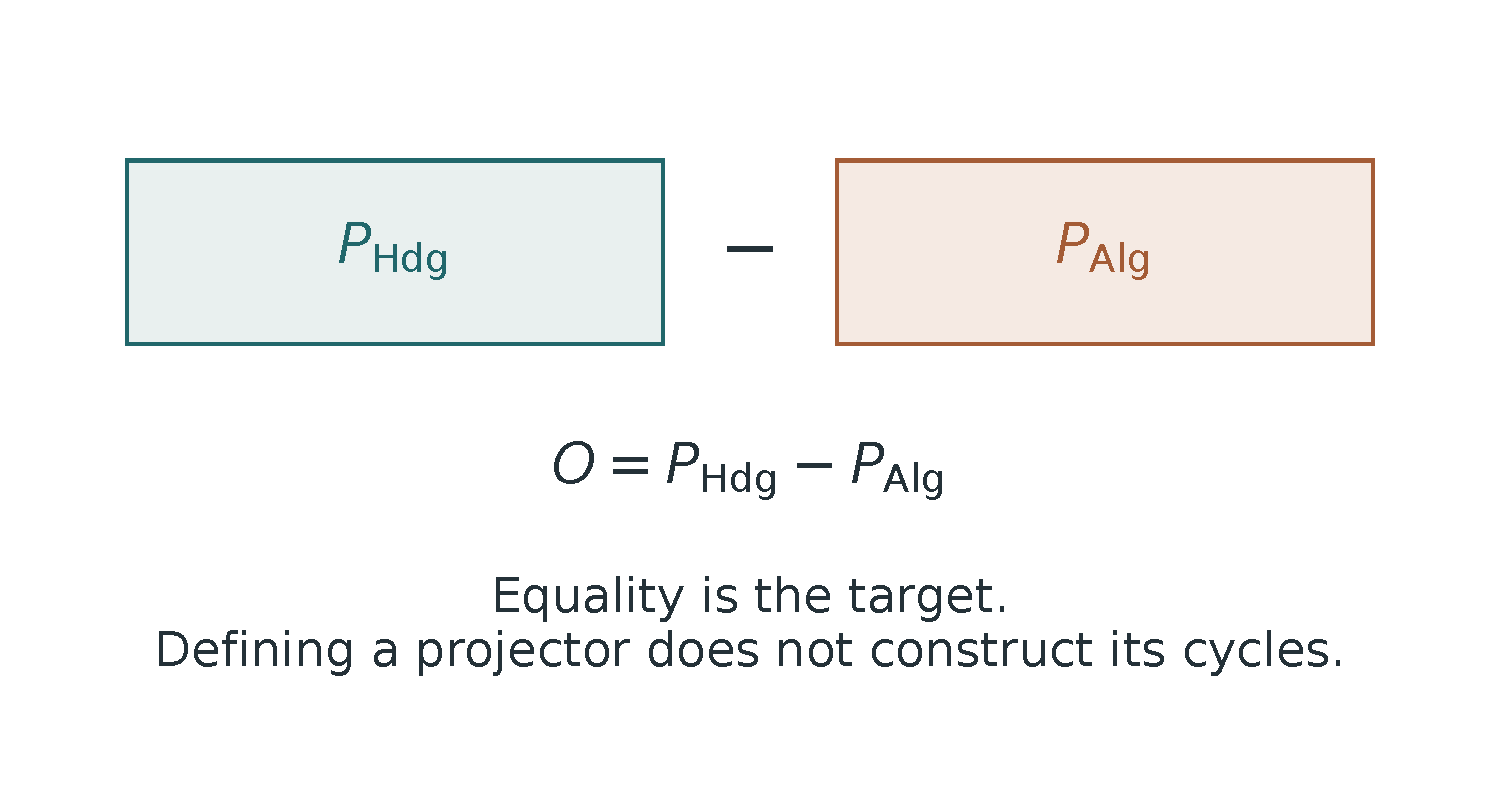
\includegraphics[width=0.98\linewidth]{04_projector_diagnostic.pdf}\caption{The real orthogonal obstruction is a diagnostic reformulation. An algebraic realization of the full Hodge projector is not supplied.}\end{figure}

\section{Why dimension four is the first focused target}
The first general unresolved middle case occurs for primitive degree-four cohomology on a smooth projective fourfold. The Hodge diamond highlights the central packet.

\begin{figure}[tbp]\centering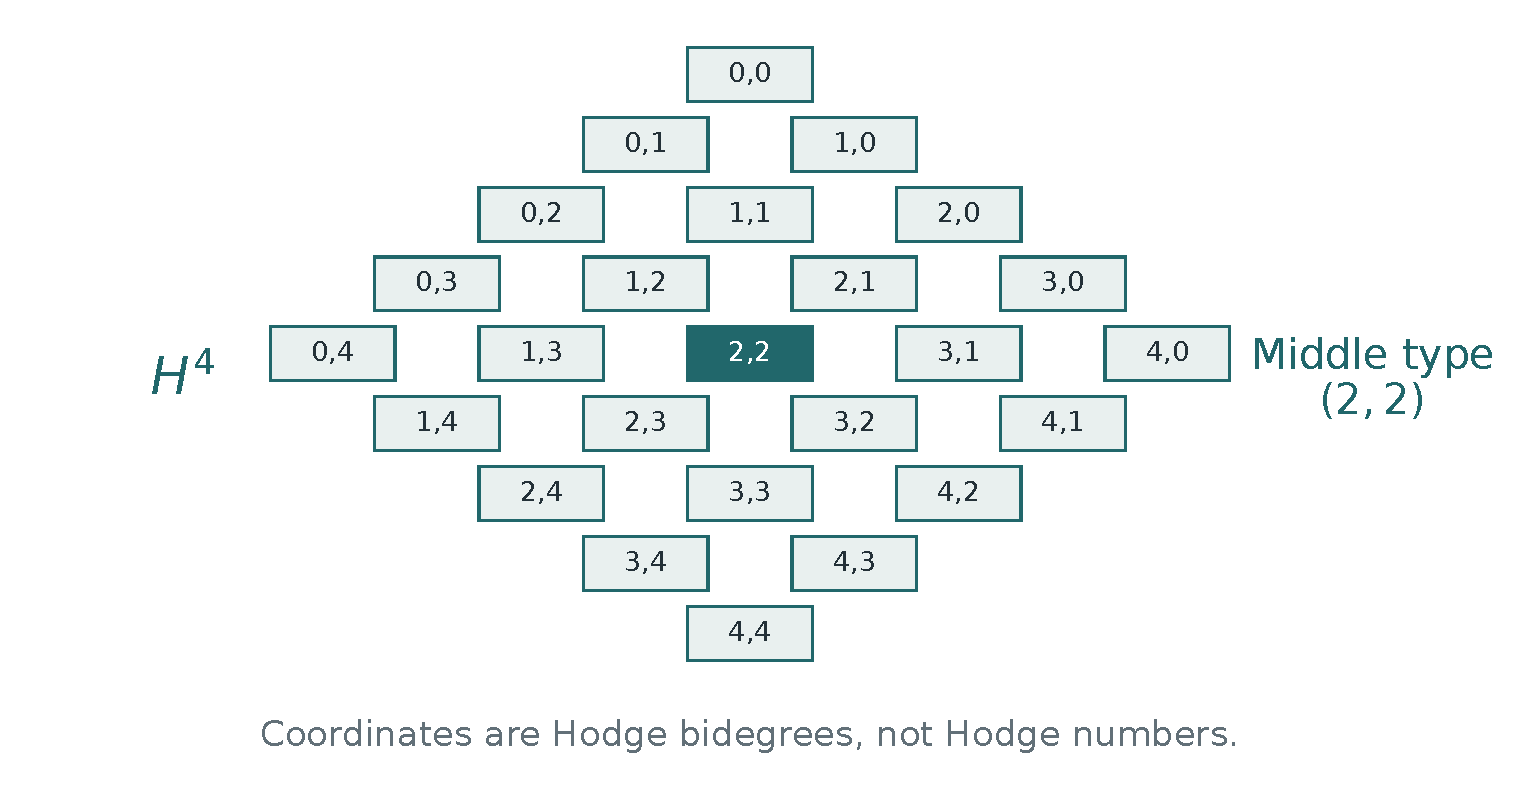
\includegraphics[width=0.98\linewidth]{03_fourfold_middle.pdf}\caption{Hodge bidegree positions for a fourfold. The diagram gives indices rather than numerical Hodge dimensions.}\end{figure}

\chapter{Primitive and coniveau reductions}
\section{Lefschetz packet decomposition}
Let $h\in H^2(X,\Q)$ be the class of an ample divisor and let $L(\alpha)=h\smile\alpha$. Hard Lefschetz and primitive decomposition yield
\[
H^{2p}(X,\Q)=\bigoplus_{r\ge0}L^rH_{\mathrm{prim}}^{2p-2r}(X,\Q).
\]
The decomposition respects Hodge type.

\begin{theorem}[Primitive reduction]
If every primitive rational Hodge class is algebraic, then every rational Hodge class is algebraic.
\end{theorem}
\begin{proof}
Write $\alpha=\sum_rL^r\alpha_r$ with each $\alpha_r$ primitive and of Hodge type. The class $h$ is algebraic. If $\alpha_r$ is algebraic, then $L^r\alpha_r=h^r\smile\alpha_r$ is algebraic. Summing gives an algebraic representative of $\alpha$.
\end{proof}

For a fourfold and $p=2$,
\[
\alpha=L\beta+\alpha_{\mathrm{prim}},
\qquad
\beta\in H^{1,1}(X)\cap H^2(X,\Q).
\]
The Lefschetz $(1,1)$ theorem makes $\beta$ algebraic. Only $\alpha_{\mathrm{prim}}$ remains.



\section{Support localization and coniveau}
Let $N^pH^{2p}(X,\Q)$ be the geometric coniveau-$p$ subspace. In degree $2p$, purity forces support contributions of codimension $p$ to be generated by fundamental classes of codimension-$p$ components.

\begin{theorem}[Degree-$2p$ coniveau identification]
For smooth projective $X$,
\[
N^pH^{2p}(X,\Q)=\Alg^p(X).
\]
\end{theorem}
\begin{proof}[Proof sketch]
The inclusion from right to left is immediate because a codimension-$p$ cycle is supported on its underlying algebraic set. Conversely, a class in coniveau $p$ is in the image of cohomology with supports in an algebraic subset $Z$ of codimension at least $p$. Contributions from components of codimension greater than $p$ vanish in degree $2p$. Purity identifies the degree-$2p$ supported contribution of each codimension-$p$ irreducible component with its fundamental class. Resolution and additivity reduce a general $Z$ to these components.
\end{proof}

Thus the conjecture is equivalently the support statement
\[
\Hdg^p(X)\subseteq N^pH^{2p}(X,\Q).
\]



\addcontentsline{toc}{part}{Part II. Algebraic cycle frames and exact polyphase refinement}

\chapter{Positive cycle-frame calculus}
\section{Analysis and synthesis}
Fix a finite family of rational algebraic cycle classes
\[
c_1,\ldots,c_N\in H^{2p}(X,\Q).
\]
Let $V\subseteq H^{2p}(X,\R)$ be the real extension of the rational Hodge packet under study. For the positive frame certificate below, require every $c_j$ to belong to $V$. This can be achieved by a rational algebraic packet projector when such a projector has been constructed. Projection through an arbitrary orthogonal Hodge projector does not establish that the projected vectors are algebraic. Define
\[
C:\R^N\to H^{2p}(X,\R),
\qquad Ce_j=c_j,
\]
and the positive frame operator
\[
S=CC^*=\sum_{j=1}^N|c_j\rangle\langle c_j|.
\]

\begin{theorem}[Finite positive cycle-frame certificate]
Let $A=\Span_{\R}\{c_1,\ldots,c_N\}$. Then
\[
\im S=A,
\qquad
\ker S=A^\perp.
\]
Under the stated containment $c_j\in V$, the selected cycles span $V$ if and only if $S|_V$ is positive definite. Without containment, positivity only detects the absence of vectors in $V$ orthogonal to the cycle span and does not prove that span contains $V$.
\end{theorem}
\begin{proof}
The equality $\im(CC^*)=\im C$ is standard. Moreover
\[
\langle v,Sv\rangle=\|C^*v\|^2=\sum_j|\langle c_j,v\rangle|^2.
\]
This vanishes exactly when $v$ is orthogonal to every cycle class.
\end{proof}

If $H$ is a matrix whose columns form an orthonormal basis of $V$, the finite Gram certificate is
\[
G=H^*SH.
\]
Under $A\subseteq V$, we have $A=V$ if and only if $\lambda_{\min}(G)>0$. Without that containment, use a rational basis matrix $H_{\Q}$ for the target and the exact certificate $\operatorname{rank}_{\Q}[C\ H_{\Q}]=\operatorname{rank}_{\Q}C$ to test $V\subseteq A$.

\begin{figure}[tbp]\centering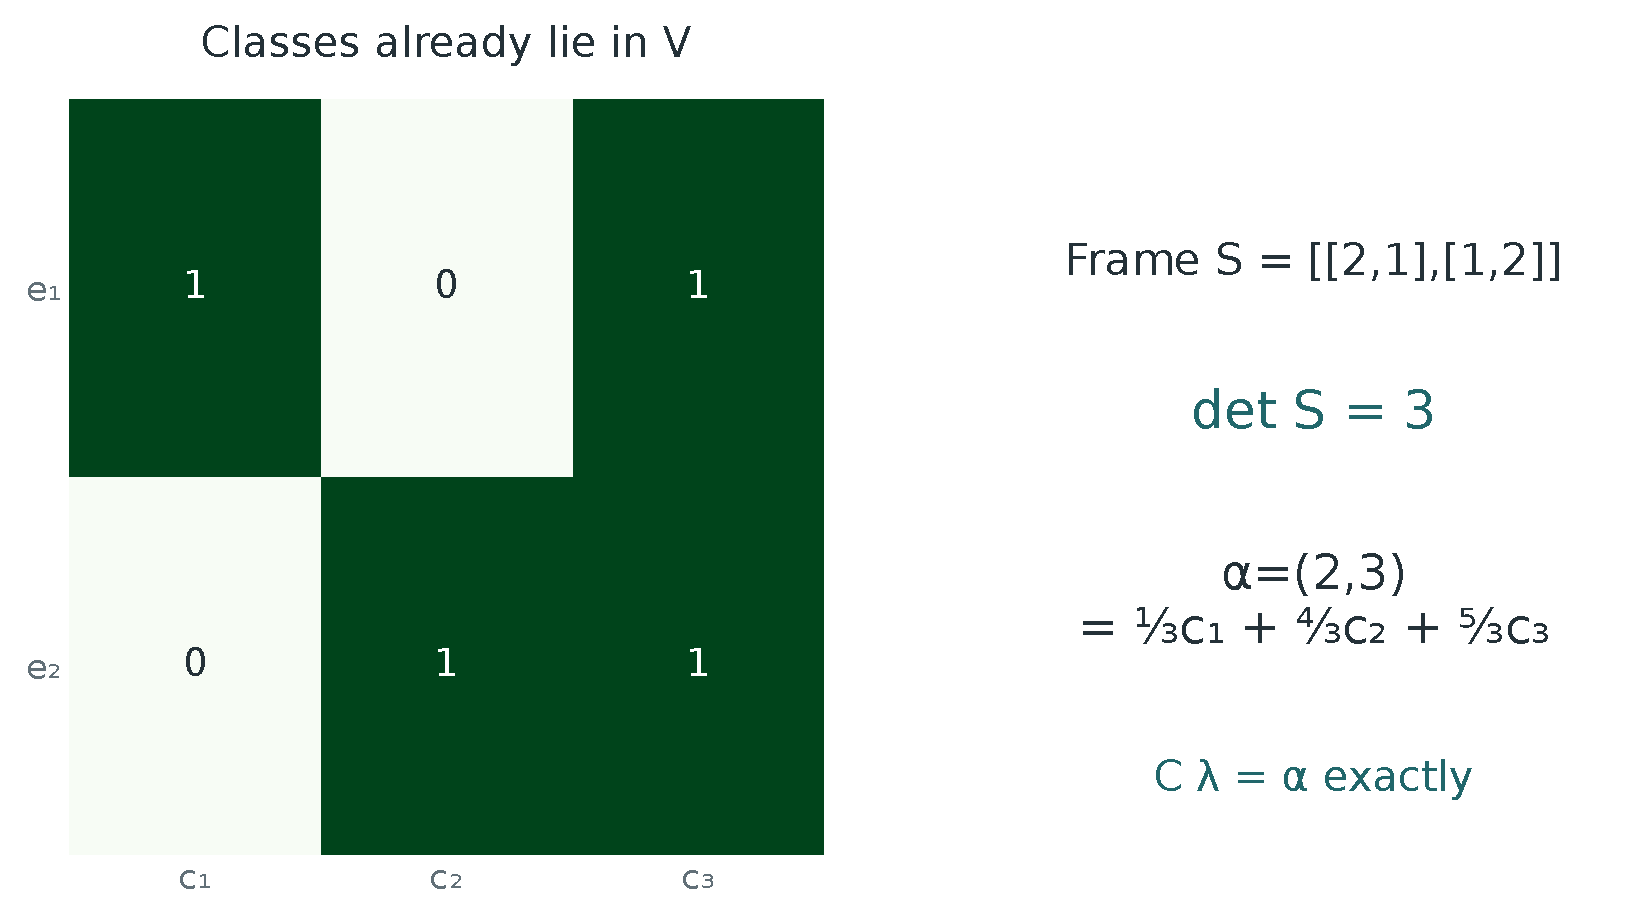
\includegraphics[width=0.98\linewidth]{06_corrected_rational_frame.pdf}\caption{A finite rational frame example with its cycle vectors contained in the selected target. Actual geometric applications must supply algebraic vectors with verified cohomology coordinates.}\end{figure}



The orthogonal synthesis of a class $\alpha$ from the cycle span is
\[
P_A\alpha=S S^\dagger\alpha.
\]
If $\alpha\in A$, this is exact.



\section{Packet assembly without false orthogonality}
Partition the cycle indices into packets $I_\lambda$. Define
\[
S_\lambda=\sum_{j\in I_\lambda}|c_j\rangle\langle c_j|.
\]
Then
\[
S=\sum_\lambda S_\lambda.
\]
No orthogonality of the child spans is assumed.

\begin{theorem}[Positive child-kernel intersection]
For any subspace $V$,
\[
\ker(S|_V)=\bigcap_\lambda\ker(S_\lambda|_V).
\]
\end{theorem}
\begin{proof}
If $Sv=0$, positivity gives
\[
0=\langle v,Sv\rangle=\sum_\lambda\langle v,S_\lambda v\rangle.
\]
Each nonnegative summand vanishes, which implies $S_\lambda v=0$. The converse is immediate.
\end{proof}

\begin{figure}[tbp]\centering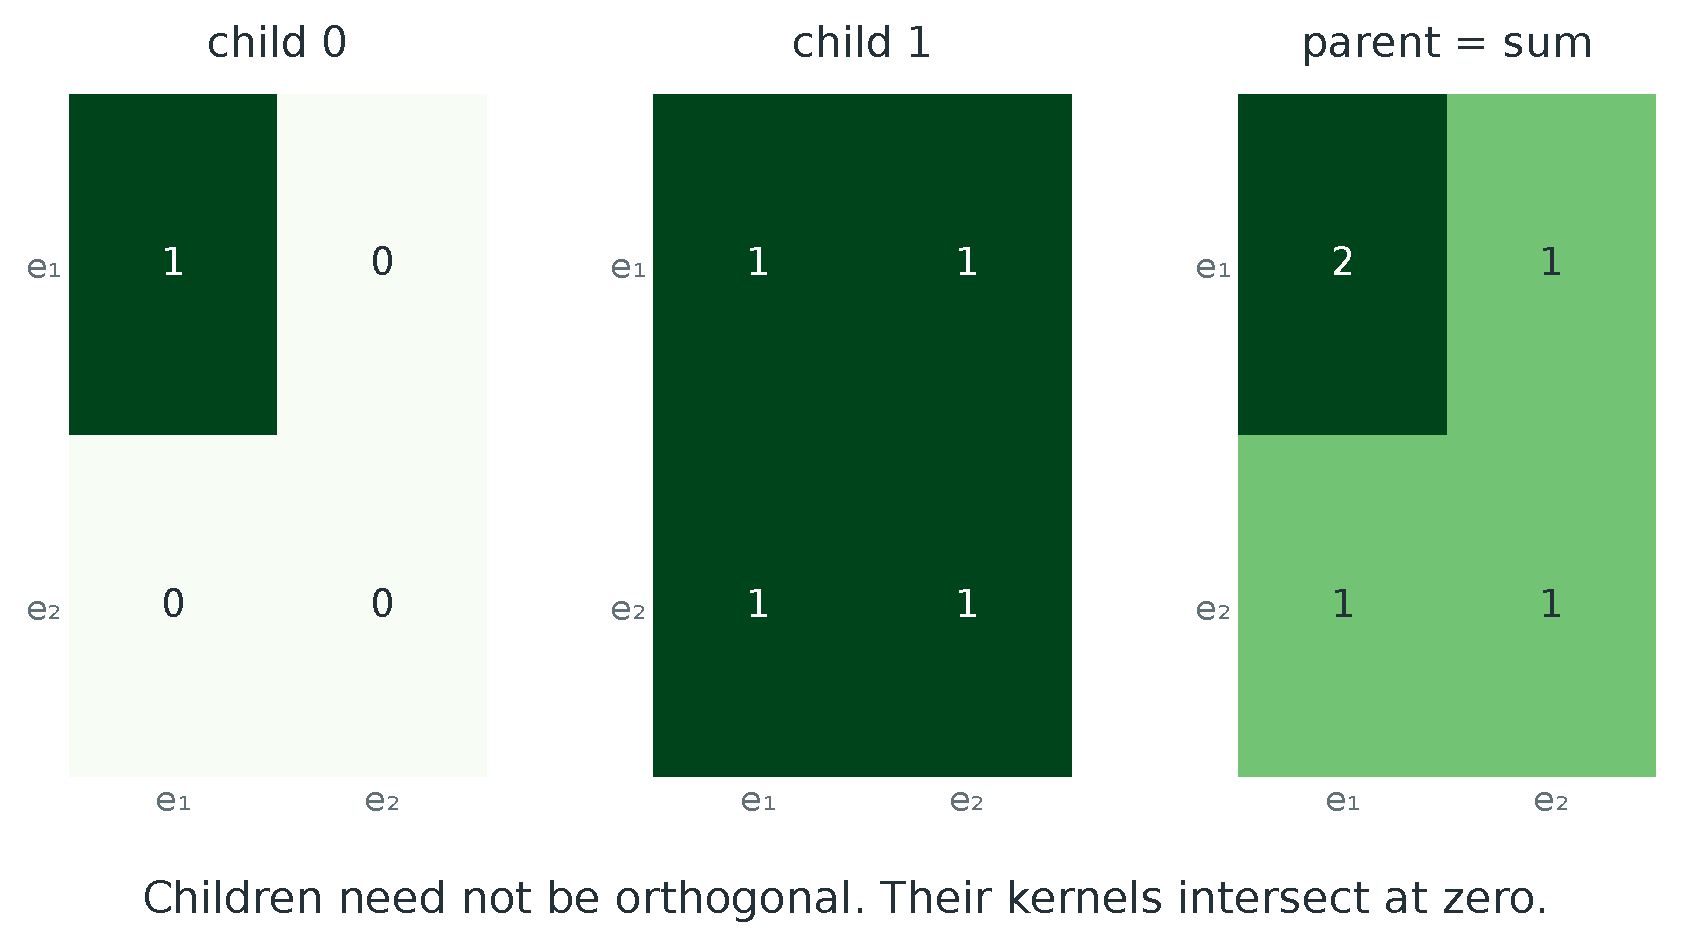
\includegraphics[width=0.98\linewidth]{07_positive_polyphase.pdf}\caption{Positive parent-child frame assembly. The identity combines frames without assuming their ranges are orthogonal.}\end{figure}

\chapter{Degree-residue polyphase refinement}
\section{Exact parent-child frame law}
Fix a projective embedding and assign each cycle its degree. For modulus $M$, define the residue packet
\[
I_{M,r}=\{j:\deg Z_j\equiv r\pmod M\},
\qquad
S_{M,r}=\sum_{j\in I_{M,r}}|c_j\rangle\langle c_j|.
\]

\begin{theorem}[Exact degree polyphase refinement]
For every positive integer $L$,
\[
S_{M,r}=\sum_{\ell=0}^{L-1}S_{LM,r+\ell M}.
\]
\end{theorem}
\begin{proof}
The congruence class $r$ modulo $M$ is the disjoint union of the classes $r+\ell M$ modulo $LM$. The rank-one frame terms are partitioned accordingly.
\end{proof}





\section{Multiaxial packet addresses}
Degree residue is only one address. A refined cycle packet may be labeled by
\[
\lambda=(r_{\mathrm{Lef}},r_{\deg},\chi_{\mathrm{mon}},s_{\mathrm{supp}},\nu_{\mathrm{Frob}}).
\]
The entries record Lefschetz depth, degree residue, monodromy or symmetry type, support stratum, and arithmetic phase. The total positive frame remains the sum of all leaves. This allows independent methods to solve different geometric sectors before exact synthesis.

\chapter{Finite saturation and exact rational closure}
For each degree cutoff $D$, let $A_D^p(X)$ be the rational span of codimension-$p$ cycle classes of degree at most $D$. Then
\[
A_1^p\subseteq A_2^p\subseteq\cdots\subseteq H^{2p}(X,\Q).
\]

\begin{theorem}[Finite stabilization]
There exists $D_0$ such that $A_D^p(X)=A_{D_0}^p(X)$ for every $D\ge D_0$.
\end{theorem}
\begin{proof}
The dimensions form a nondecreasing sequence of integers bounded by $\dim H^{2p}(X,\Q)$. Only finitely many strict increases are possible.
\end{proof}

\begin{corollary}[Approximation becomes exact]
Let $P_D$ be the orthogonal projector onto $A_D^p(X)\otimes\R$. For a rational class $\alpha$,
\[
\lim_{D\to\infty}\|(I-P_D)\alpha\|=0
\]
if and only if $\alpha\in A_D^p(X)$ for some finite $D$.
\end{corollary}
\begin{proof}
After stabilization, the residual is constant. A constant tail converging to zero is zero.
\end{proof}

Because the matrices and target vector can be chosen over $\Q$, real membership implies rational membership by row reduction over $\Q$.



\begin{resultbox}[Finite completion certificate]
If $H$ is a rational basis matrix of $\Hdg^p(X)$ and $C_D$ is the cycle matrix, then the Hodge conjecture for $(X,p)$ is equivalent to the existence of $D$ with
\[
\rank_{\Q} C_D=\rank_{\Q}[C_D\ H].
\]
A positive compressed frame is equivalent only when the supplied cycle vectors lie in the target packet, or when a separately verified invariant restriction supplies the required containment. The rank equality is valid without that extra hypothesis.
\end{resultbox}

\addcontentsline{toc}{part}{Part III. Support packets and correspondence reconstruction}

\chapter{Support verification and multiplicity recovery}
Let $Z\subseteq X$ be a closed algebraic subset and $j:X\setminus Z\hookrightarrow X$. The support exact sequence contains
\[
H_Z^{2p}(X,\Q)\longrightarrow H^{2p}(X,\Q)\xrightarrow{j^*}H^{2p}(X\setminus Z,\Q).
\]

\begin{theorem}[Exact support test]
A class $\alpha\in H^{2p}(X,\Q)$ is supported on $Z$ if and only if $j^*\alpha=0$.
\end{theorem}
\begin{proof}
This is exactness at the middle term.
\end{proof}

\begin{figure}[tbp]\centering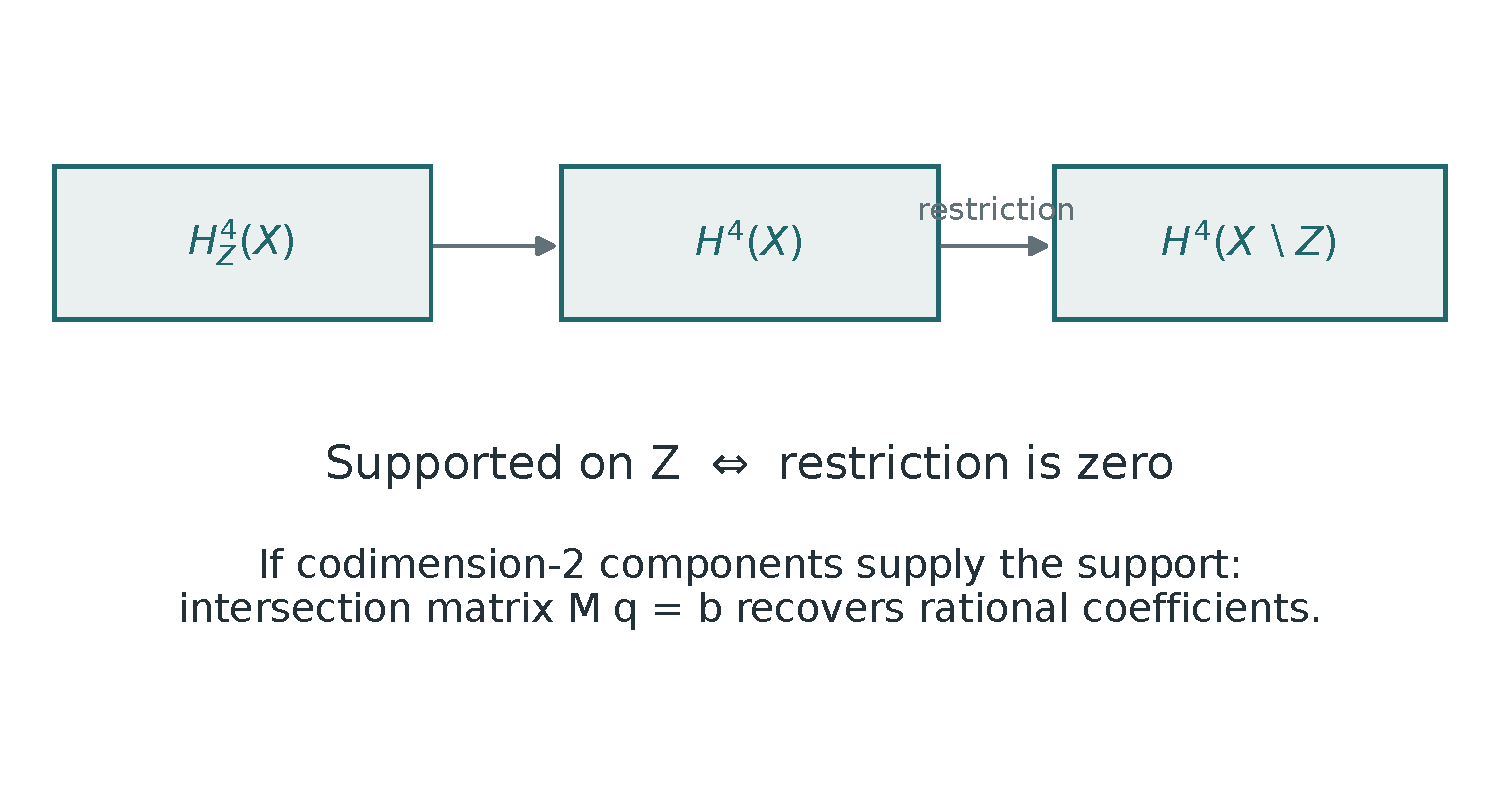
\includegraphics[width=0.98\linewidth]{08_support_verification.pdf}\caption{The restriction-to-complement test verifies a supplied support. It does not construct a support for an arbitrary Hodge class.}\end{figure}

Suppose $Z$ has codimension at least $p$ and its codimension-$p$ components are $Z_1,\ldots,Z_r$. Purity gives
\[
\alpha=\sum_{i=1}^r q_i[Z_i].
\]
Choose complementary test classes $\gamma_k$ and define
\[
M_{ki}=\int_X[Z_i]\smile\gamma_k,
\qquad
b_k=\int_X\alpha\smile\gamma_k.
\]
Then $Mq=b$. Removing dependent columns yields exact rational multiplicities.



\chapter{Divisor-lowering correspondence channels}
\section{Degree bookkeeping}
Let $X$ have complex dimension $n$, let $V\subseteq H_{\mathrm{prim}}^{2p}(X,\Q)$ be a rational Hodge substructure, and let $Y_r$ be smooth projective. Choose correspondences
\[
\Gamma_r\in\CH^{n-p+1}(X\times Y_r)_{\Q},
\qquad
\Lambda_r\in\CH^{\dim Y_r+p-1}(Y_r\times X)_{\Q}.
\]
They induce
\[
A_r=(\Gamma_r)_*:V\to H^2(Y_r,\Q),
\qquad
B_r=(\Lambda_r)_*:H^2(Y_r,\Q)\to H^{2p}(X,\Q).
\]
Algebraic correspondences preserve rationality and shift Hodge type by the required bidegree.

\begin{theorem}[Invertible divisor-lowering transfer]
Suppose
\[
T=\sum_{r=1}^M B_rA_r
\]
preserves $V$ and is invertible on $V$. Then every rational Hodge class in $V$ is algebraic.
\end{theorem}
\begin{proof}
Let $\alpha\in V$ be of type $(p,p)$. Each $A_r\alpha$ is rational of type $(1,1)$ on $Y_r$, hence is the class of a rational divisor $D_r$ by the Lefschetz $(1,1)$ theorem. Therefore
\[
T\alpha=\sum_r(\Lambda_r)_*[D_r]
\]
is algebraic on $X$.

Let $\chi_T(t)=t^d+c_{d-1}t^{d-1}+\cdots+c_0$ be the characteristic polynomial on $V$. Invertibility means $c_0\ne0$. Cayley-Hamilton gives
\[
T^{-1}=-\frac{1}{c_0}\bigl(T^{d-1}+c_{d-1}T^{d-2}+\cdots+c_1I\bigr).
\]
Each power of $T$ is induced by compositions and rational sums of algebraic correspondences. Thus $T^{-1}$ preserves algebraic cycle classes. Hence $\alpha=T^{-1}(T\alpha)$ is algebraic.
\end{proof}

\begin{figure}[tbp]\centering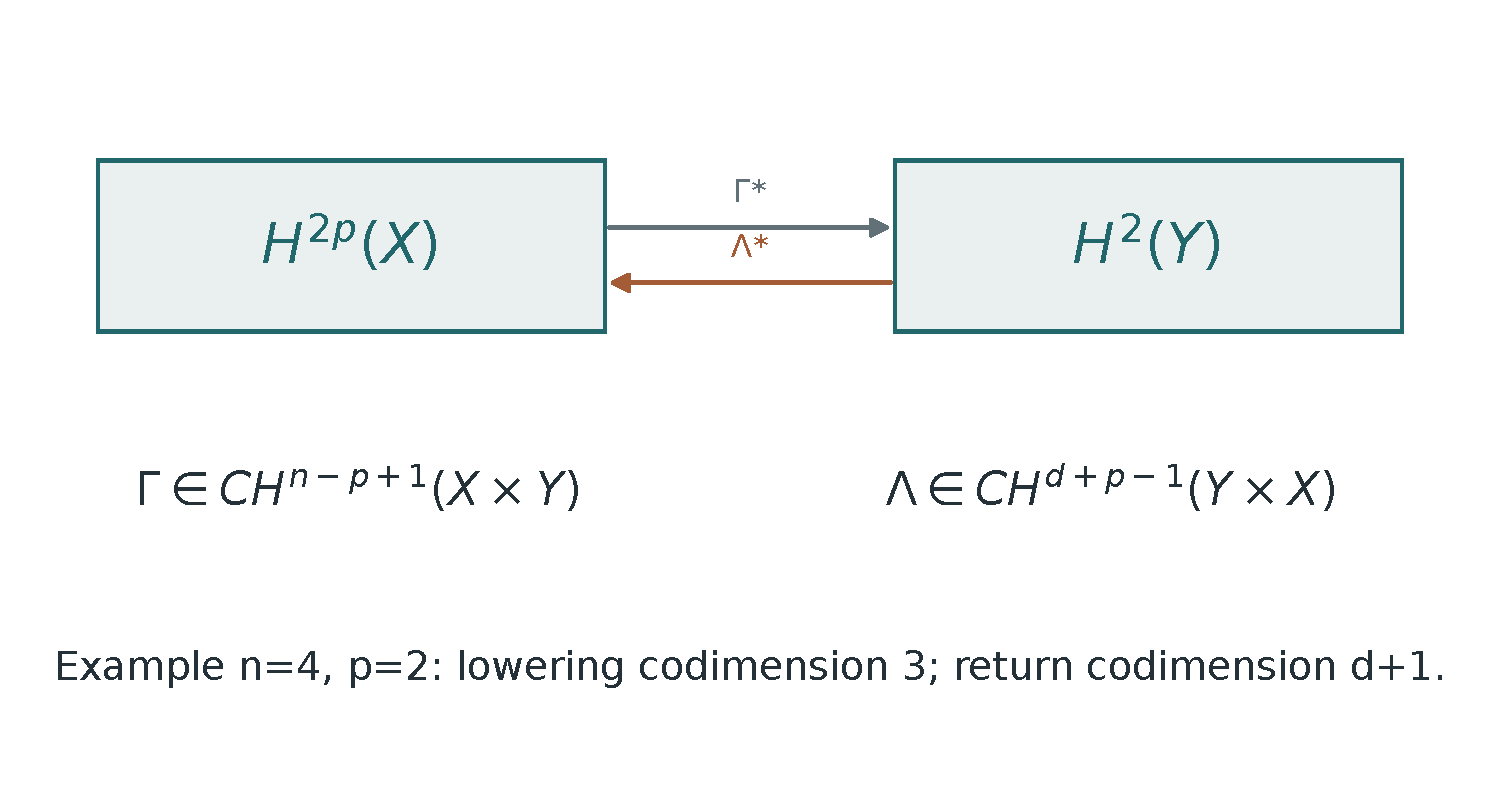
\includegraphics[width=0.98\linewidth]{09_correspondence_degrees.pdf}\caption{The exact degree shifts required for lowering to divisor degree and returning. Actual Chow kernels and invertibility are additional inputs.}\end{figure}

\begin{figure}[tbp]\centering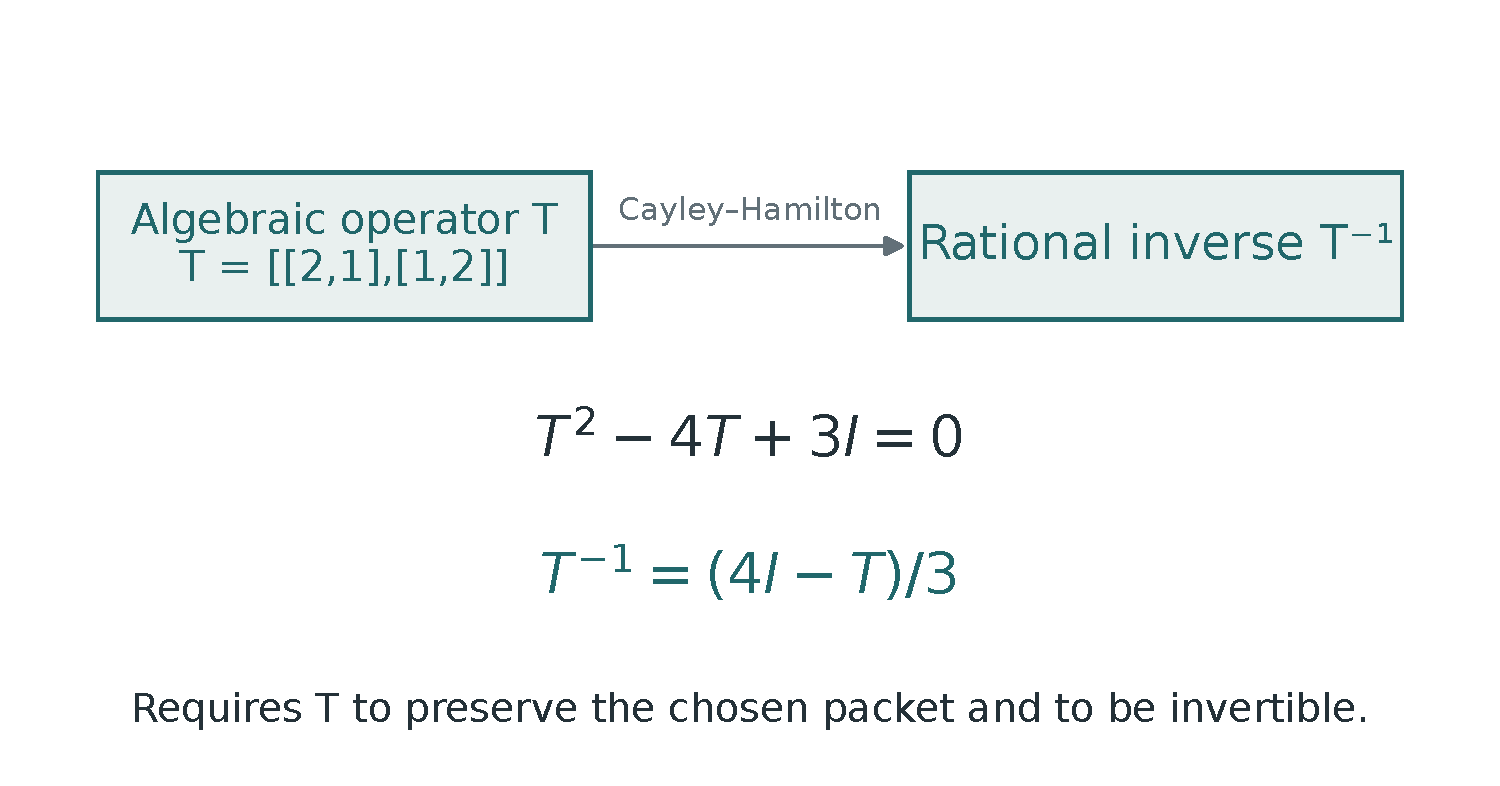
\includegraphics[width=0.98\linewidth]{10_rational_inverse.pdf}\caption{A finite rational example of polynomial inversion. The geometric theorem requires the operator to be induced by algebraic correspondences.}\end{figure}

\section{Positive multi-channel form}
Assume the polarized adjoint $A_r^\dagger$ is realized by an algebraic return correspondence $B_r$. This is an additional geometric hypothesis, not an automatic consequence in arbitrary settings. Then
\[
T=\sum_rA_r^\dagger A_r
\]
is positive and
\[
\langle v,Tv\rangle=\sum_r\|A_rv\|^2.
\]
Therefore
\[
\ker T=\bigcap_r\ker A_r.
\]
Joint injectivity of the lowering channels is enough.





\begin{corollary}[Finite Gram certificate]
Choose a rational basis $e_1,\ldots,e_d$ of $V$. If
\[
G_{ij}=\sum_r\langle A_re_i,A_re_j\rangle_{Y_r}
\]
has nonzero determinant, every rational Hodge class in $V$ is algebraic.
\end{corollary}

\chapter{Family propagation}
Let $\pi:\mathcal X\to S$ and $\rho_r:\mathcal Y_r\to S$ be smooth projective families over a connected base. Relative algebraic correspondences induce morphisms of Gauss-Manin local systems. In a flat rational trivialization, their transfer matrix is constant.

\begin{theorem}[Propagation of invertibility]
If a relative transfer $T_s$ is invertible on one fiber $s_0$, it is invertible on every fiber in the connected base on which the local systems and correspondences are defined.
\end{theorem}
\begin{proof}
The determinant of the constant rational matrix representing the local-system morphism is locally constant. It is nonzero at $s_0$, hence everywhere on the connected base.
\end{proof}



\addcontentsline{toc}{part}{Part IV. Closed branches and classical validation cases}

\chapter{Geometric closure rules}
\section{Affine pavings}
\begin{theorem}[Affine-paving branch]
If $X$ admits a finite filtration whose successive differences are affine spaces, then the cycle class map
\[
\CH^p(X)_{\Q}\to H^{2p}(X,\Q)
\]
is surjective for every $p$.
\end{theorem}
\begin{proof}[Proof sketch]
Induct through the filtration using localization for Chow groups and cohomology. Each affine cell contributes one even-degree generator represented by the closure of that cell. No odd cohomology is introduced.
\end{proof}

\section{Projective bundles, blow-ups, and descent}
\begin{proposition}[Projective-bundle closure]
If the rational Hodge conjecture holds for $X$, it holds for $\mathbb P(E)\to X$.
\end{proposition}
\begin{proof}
The projective-bundle formula expresses cohomology as a direct sum of powers of the algebraic hyperplane class times pullbacks of cohomology from $X$.
\end{proof}

\begin{proposition}[Blow-up closure]
If it holds for $X$ and a smooth center $Z$, it holds for $\operatorname{Bl}_ZX$.
\end{proposition}
\begin{proof}
Use the standard blow-up cohomology decomposition. The new summands are Tate twists of cohomology from $Z$ multiplied by powers of the algebraic exceptional divisor.
\end{proof}

\begin{proposition}[Generically finite descent]
Let $f:Y\to X$ be proper and generically finite of degree $d$ between smooth projective varieties of equal dimension. If the conjecture holds for $Y$, it holds for $X$.
\end{proposition}
\begin{proof}
For a Hodge class $\alpha$ on $X$, the pullback $f^*\alpha$ is algebraic on $Y$. Push forward and use $f_*f^*\alpha=d\alpha$.
\end{proof}



\chapter{Cubic fourfolds as a validation of the transfer theorem}
Let $X\subset\mathbb P^5$ be a smooth cubic fourfold and let $F(X)$ be its Fano variety of lines. The universal incidence variety
\[
P=\{(\ell,x):x\in\ell\}\subset F(X)\times X
\]
induces the Abel-Jacobi map
\[
A=p_*q^*:H^4_{\mathrm{prim}}(X,\Q)\to H^2_{\mathrm{prim}}(F(X),\Q).
\]
Beauville and Donagi proved that this is a polarized Hodge isomorphism up to the standard twist \cite{BeauvilleDonagi}. The polarized adjoint is represented by an algebraic incidence return after inserting the appropriate power of the Pluecker class. Therefore the divisor-lowering transfer is invertible.

\begin{resultbox}[Classical validation]
A primitive rational $(2,2)$ class on a cubic fourfold is sent to a rational $(1,1)$ class on $F(X)$, represented by a divisor. The algebraic return correspondence and its polynomial inverse reconstruct an algebraic codimension-two class on $X$. This is a validation of the packet criterion, not a claim of a new proof of the classical cubic-fourfold result.
\end{resultbox}





\chapter{Gushel-Mukai validation channels}
Debarre and Kuznetsov construct line and plane incidence correspondences relating vanishing middle cohomology of suitable Gushel-Mukai varieties to primitive degree-two cohomology of associated double EPW sextics \cite{DebarreKuznetsov}. In the ranges where the polarized Hodge isomorphisms are established, the same divisor-lowering theorem applies.

\begin{itemize}
\item For suitable GM fourfolds, the vanishing $H^4$ packet is lowered by universal lines to divisor degree.
\item For suitable GM sixfolds, the vanishing $H^6$ packet is lowered by universal planes to divisor degree.
\item Ambient and tautological classes are treated separately and are algebraic.
\end{itemize}



\addcontentsline{toc}{part}{Part V. The analytic and K-theoretic branch}

\chapter{Hodge packets in topological K-theory}
For finite CW complexes, the rational topological Chern character gives
\[
\operatorname{ch}_{\mathrm{top}}:K^0_{\mathrm{top}}(X)\otimes\Q\xrightarrow{\sim}H^{\mathrm{even}}(X,\Q).
\]
For smooth projective $X$, the algebraic Chern character identifies algebraic $K$-theory rationally with the Chow ring after the usual filtration. Thus the rational Hodge conjecture for all degrees is equivalent to algebraization of topological $K$-classes whose Chern-character components are rational Hodge classes \cite{AtiyahHirzebruch}.

\section{Adams degree projectors}
For integer $m\ge2$, Adams operations satisfy
\[
\operatorname{ch}_q(\psi^m\xi)=m^q\operatorname{ch}_q(\xi).
\]
Define
\[
e_p^{(m)}=\prod_{\substack{0\le q\le\dim X\\q\ne p}}
\frac{\psi^m-m^qI}{m^p-m^q}.
\]
Then
\[
\operatorname{ch}_q(e_p^{(m)}\xi)=\delta_{pq}\operatorname{ch}_p(\xi).
\]
This exactly isolates codimension $p$ inside a topological $K$-packet.



\chapter{Nonlinear Dolbeault obstruction packets}
Let $E$ be a smooth complex bundle and consider a candidate $(0,1)$-connection. After gauge fixing, write the integrability equation abstractly as
\[
F(a)=f+La+B(a,a)=0,
\]
where $L$ is the linearized operator and $B$ is a bounded bilinear term. Assume a Fredholm splitting of the target
\[
I=Q+\Pi,
\]
where $Q$ projects onto the closed range of $L$ and $\Pi$ onto a finite-dimensional obstruction space. Choose a gauge-fixed complement to $\ker L$ as the domain and let $R$ be a right inverse of $L$ taking values in that complement. Use norms on the projected data for which $\|QB(a,b)\|\le C\|a\|\|b\|$.

\begin{theorem}[Range-packet contraction]
Assume
\[
\|R\|\le M,
\qquad
\|B(a,b)\|\le C\|a\|\|b\|,
\qquad
4CM^2\|Qf\|<1.
\]
Then the map
\[
\mathcal T(a)=-RQ(f+B(a,a))
\]
has a unique fixed point in the gauge-fixed ball $\|a\|\le2M\|Qf\|$. If $Qf=0$, the ball is the singleton $\{0\}$ and the range solution is immediate. At the fixed point, the range component of $F(a)$ vanishes. The remaining obstruction is
\[
\Phi=\Pi(f+B(a,a)).
\]
The full integrability equation holds if and only if $\Phi=0$.
\end{theorem}
\begin{proof}
For $\|a\|\le r=2M\|Qf\|$,
\[
\|\mathcal T(a)\|\le M\|Qf\|+MC r^2\le r
\]
under the stated bound. Moreover
\[
\|\mathcal T(a)-\mathcal T(b)\|
\le MC(\|a\|+\|b\|)\|a-b\|.
\]
The Lipschitz constant is strictly less than one on the stated ball.
Banach's fixed-point theorem gives the solution. Applying $Q$ to the equation proves range cancellation. The remaining component is precisely $\Phi$.
\end{proof}





\section{A positive spectral microscope}
Large ample twists can make integrability defects visible in the asymptotic degree distribution of Dolbeault-Dirac kernels. Charbonneau and Stern obtain asymptotic Hodge filtrations in which positive coefficients depend on powers of $F_A^{0,2}$ \cite{CharbonneauStern}. Schematically,
\[
\Tr(P_{2j}\Pi_{A,k})
=c_{n,j}k^{n-2j}\|(F_A^{0,2})^{\wedge j}\|_{L^2}^2+O(k^{n-2j-1}),
\qquad c_{n,j}>0.
\]
This detects nonintegrability. It does not by itself remove the defect.



\section{Trace blindness and the true missing bridge}
Chern characters control traces of powers of curvature. An endomorphism-valued obstruction can be nonzero while all such trace moments vanish. For example, $N=\left(\begin{smallmatrix}0&1&0\\0&0&1\\0&0&0\end{smallmatrix}\right)$ is nonzero, while $N^3=0$ and $\operatorname{Tr}(N^r)=0$ for every positive integer $r$. This is the elementary negative control.



\begin{openproblem}[Analytic bridge]
The unresolved analytic theorem is not the range equation. It is a positive saturation statement forcing the finite obstruction packet $\Phi$ to vanish for every rational Hodge $K$-packet after allowable stabilization. Proving that statement in general would be essentially a K-theoretic form of the Hodge conjecture.
\end{openproblem}

\section{Consequences of the obstruction split}
The obstruction split prevents a common logical error. Solving the projected range equation does not solve the original integrability problem unless the complementary packet also vanishes. The calculus therefore records three distinct outcomes. First, if $\Pi=0$, the problem is unobstructed and the contraction theorem gives an actual integrable structure. Second, if $\Pi\ne0$ but $\Phi=0$ for geometric reasons, the correction again closes. Third, if $\Phi\ne0$, the method has produced a finite certificate explaining exactly why that representative cannot be algebraized by the chosen deformation.

This creates a practical research program. One can refine the finite obstruction space by symmetry, monodromy, support, or arithmetic phase, obtaining
\[
\Phi=\sum_{\lambda}\Phi_{\lambda}.
\]
Since the decomposition is complete, integrability is equivalent to the simultaneous vanishing of all children. Different geometric arguments may eliminate different children. A symmetry packet may vanish by representation theory, a support packet by localization, and an arithmetic packet by compatibility across reductions. The analytic branch therefore remains useful even before the general bridge is proved: it supplies exact special-case theorems whenever all obstruction children can be eliminated.

The negative controls are equally important. Ample twisting can amplify $F_A^{0,2}$ in a spectral observable without reducing it. Direct-sum stabilization adds positive defect energies for block-diagonal connections. Trace identities may miss nilpotent components. These facts rule out several tempting but invalid shortcuts and keep the remaining theorem sharply stated.


\addcontentsline{toc}{part}{Part VI. Atomic status ledger and focused next theorem}

\chapter{Dependency graph and proof status}
The project separates proved statements, classical inputs, conditional mechanisms, and open bridges.



\begin{longtable}{p{0.40\textwidth}p{0.16\textwidth}p{0.34\textwidth}}
\caption{Atomic status ledger.}\label{tab:status}\\
\toprule
Statement & Status & Boundary \\
\midrule
\endfirsthead
\toprule
Statement & Status & Boundary \\
\midrule
\endhead
Master obstruction projector & Proved & Finite-dimensional linear algebra \\
Primitive Lefschetz reduction & Proved & Uses hard Lefschetz and algebraicity of the polarization \\
Degree-$2p$ coniveau identification & Proved & Rational coefficients and purity \\
Positive cycle-frame certificate & Corrected & Requires explicit algebraic cycles contained in the selected packet \\
Exact degree polyphase assembly & Proved & Frame operators, not sums of span projectors \\
Finite saturation of bounded-degree spans & Proved & Non-effective degree bound \\
Support verification & Proved & Candidate support must already be supplied \\
Multiplicity reconstruction & Proved & Finite rational linear algebra \\
Divisor-lowering transfer theorem & Proved & Requires explicit algebraic correspondences and invertibility \\
Positive multi-channel criterion & Conditional & Algebraic realization of polarized adjoints is an extra hypothesis \\
Family propagation & Proved & Relative correspondences over a connected smooth base \\
Affine-paving branch & Proved & Classical localization argument \\
Projective bundle, blow-up, descent rules & Proved & Standard cohomological decompositions \\
Cubic and GM channels & Classical validation & Depend on established incidence Hodge isomorphisms \\
Adams degree projector & Proved & Rational topological K-theory \\
Range-packet nonlinear correction & Proved under hypotheses & Closed range, right inverse, and contraction bound \\
Vanishing of every harmonic obstruction packet & Open & Main analytic bridge \\
Primitive fourfold multi-incidence saturation & Open & Main geometric target \\
General rational Hodge conjecture & Open & No general cycle-generation theorem is claimed \\
\bottomrule
\end{longtable}



\chapter{A focused multi-incidence target}
Let $X$ be a special smooth projective fourfold. Construct algebraic lowering channels from families of subvarieties:
\[
A_{\mathrm{line}},
A_{\mathrm{conic}},
A_{\mathrm{plane}},
A_{\mathrm{exceptional}}.
\]
The exact target is
\[
\ker A_{\mathrm{line}}
\cap\ker A_{\mathrm{conic}}
\cap\ker A_{\mathrm{plane}}
\cap\ker A_{\mathrm{exceptional}}=\{0\}
\]
on primitive degree-four cohomology. Under algebraic adjoint hypotheses, equivalently prove
\[
T_{\mathrm{tot}}
=\sum_rA_r^\dagger A_r
\quad\text{satisfies}\quad
\lambda_{\min}(T_{\mathrm{tot}})>0.
\]



\section{Why this target is realistic}
The problem is finite after the geometry is chosen:
\begin{enumerate}
\item compute the primitive cohomology representation and its symmetry decomposition
\item construct the incidence correspondences and their action
\item split the action into monodromy or symmetry packets
\item compute the joint kernel or positive Gram matrix over $\Q$
\item prove exact nonvanishing through rational rank, representation theory, or a dual certificate
\item invoke the divisor-lowering theorem to reconstruct cycles
\end{enumerate}
No single incidence family must be complete. Polyphase analysis permits separate geometric mechanisms to occupy separate primitive sectors.


\section{Three exact certificate forms}
Once the incidence channels have been constructed, the saturation statement admits three finite certificates. The geometric form is the kernel identity
\[
\bigcap_r\ker A_r=\{0\}.
\]
When algebraic correspondences realize the polarized adjoints, the equivalent positive form is
\[
\lambda_{\min}\left(\sum_rA_r^\dagger A_r\right)>0.
\]
In a rational basis, the final exact proof object is full column rank of the vertically stacked channel matrix. The kernel form explains the geometry, the positive form is stable for numerical scouting, and the rational rank form is appropriate for symbolic certification.

Two negative controls should accompany the proof. First, remove one channel at a time and recompute the joint kernel. If the kernel grows, the omitted incidence family is genuinely necessary. Second, refine a parent channel into geometric children and verify that their positive transfers sum exactly to the parent. This separates true packet coverage from accidental numerical invertibility.

A complete result should identify which primitive symmetry packets are detected by lines, conics, planes, or exceptional strata. The proof then becomes a finite occupancy statement: every primitive packet must be detected at least once. That structural description is more informative than a determinant alone and is the form most likely to propagate through families and degenerations.

\chapter{Computational and formal proof workflow}
Numerical experiments can scout candidate families but cannot replace an exact rank certificate. The intended pipeline is:
\[
\begin{aligned}
\text{exact incidence data}
&\longrightarrow \text{rational cohomology basis}
\longrightarrow \text{packet transfer matrices}\\
&\longrightarrow \text{rank or positivity certificate}
\longrightarrow \text{symbolic theorem proof}.
\end{aligned}
\]



\section{Reproducible finite checks}
The accompanying Python generator produces all figures and runs eighteen independent finite checks covering:
\begin{itemize}
\item frame idempotency and range rank
\item positive Hodge Gram spectrum
\item exact modulo-$2$ and modulo-$4$ polyphase assembly
\item positive transfer rank and energy identities
\item Cayley-Hamilton inversion
\item contraction of the removable nonlinear packet
\item Adams projector idempotency and degree isolation
\item nilpotent trace blindness
\item support multiplicity recovery
\item finite rank stabilization
\end{itemize}
These tests verify the finite examples and implementation. They do not establish the open geometric saturation theorem.

\compactpart{Part VII. Fermat Fourfold Character Packets and the Constructive Program}

\chapter{Correct scope and claim boundary}
The projector-resolved Hodge calculus naturally specializes to Fermat fourfolds
\[
X_m^4=\{x_0^m+x_1^m+x_2^m+x_3^m+x_4^m+x_5^m=0\}\subset\mathbf P^5,
\qquad m\ge 3.
\]
The diagonal symmetry group makes the primitive middle cohomology unusually explicit: it splits into one-dimensional complex character lines, and rational Hodge packets are finite Galois orbits of those lines. This permits exact symbolic analysis of individual addresses, conductors, local prime phases, and candidate algebraic correspondences. A complete classification at every mixed conductor is a separate coverage problem.

\begin{claimboundary}
The general rational Hodge conjecture remains open. For Fermat fourfolds, however, Kang is cited in the checked later literature as proving the relevant generalized Hodge statement in arbitrary degree \cite{KangFermat}. This complete edition therefore distinguishes two questions:
\begin{enumerate}
\item \emph{Existence}: does every rational Fermat $(2,2)$ class have an algebraic representative?
\item \emph{Construction}: can one write an explicit packet-resolved algebraic cycle or correspondence for every character orbit?
\end{enumerate}
The present Fermat program is primarily constructive. Its new proof objects are conductor projectors, exact packet identities, explicit Delsarte maps, weighted dyadic refinements, the proposed all-degree trivalent-tree classification, CRT--Kummer phase factorizations, and explicit CM carrier data. The relation between that existence theorem and later packet-specific combinatorial work should be stated explicitly in any publication.
\end{claimboundary}



The constructive objective is
\begin{resultbox}[Packet-resolved construction target]
For every rational packet
\[
W\subset H^4_{\mathrm{prim}}(X_m^4,\Q)\cap H^{2,2},
\]
construct
\[
Z_W\in\CH^2(X_m^4)_\Q
\qquad\text{with}\qquad
[Z_W]\ne0\text{ in }W.
\]
\end{resultbox}
Once one nonzero algebraic vector is produced in a rational irreducible diagonal-symmetry packet, the entire rational orbit is algebraic.

\chapter{Universal balanced-packet equations}
Let
\[
U_m=(\mathbf Z/m\mathbf Z)^\times
\]
and let \(\langle r\rangle_m\in\{1,\ldots,m\}\) denote the least positive residue, with \(\langle r\rangle_m=m\) when \(m\mid r\). A primitive character address is a six-tuple
\[
a=(a_0,\ldots,a_5),\qquad 1\le a_i<m,
\qquad \sum_i a_i\equiv0\pmod m.
\]
The Hodge level of the conjugate indexed by \(u\in U_m\) is
\[
\ell_a(u)=\frac1m\sum_{i=0}^5\langle ua_i\rangle_m.
\]
The character line has type \((2,2)\) exactly when \(\ell_a(1)=3\). Its rational Galois orbit is a Hodge packet exactly when
\begin{equation}\label{eq:legacy-7.1}
\boxed{
\ell_a(u)=3\qquad\forall u\in U_m.
}\end{equation}

To remove coordinate permutations, introduce the count vector
\[
n(a)=(n_1,\ldots,n_{m-1})\in\mathbf N^{m-1},
\qquad n_r=\#\{i:a_i=r\}.
\]
Let
\[
R_m(u,r)=\langle ur\rangle_m.
\]
Then the complete balanced six-packet space is the finite integer set
\begin{equation}\label{eq:legacy-7.2}
\boxed{
\mathcal B_m=
\left\{
 n\in\mathbf N^{m-1}:
 \mathbf1^Tn=6,
 \quad R_mn=3m\,\mathbf1
\right\}.
}\end{equation}
The unit group permutes the residue coordinates. After additionally identifying coordinate permutations by algebraic automorphisms, the count-vector descriptions correspond to \(U_m\)-orbits in \(\mathcal B_m\). The dimension of a fixed rational character packet is computed from distinct ordered unit conjugates before this permutation quotient.



\section{Centered Fourier form}
Define
\[
\rho_m(r)=\langle r\rangle_m-\frac m2,
\qquad
F_a(u)=\sum_i\rho_m(ua_i).
\]
Then \(a\) is balanced if and only if \(F_a(u)=0\) for all units. Moreover,
\[
F_a(-u)=-F_a(u),
\]
so only odd characters occur. For a Dirichlet character \(\chi\) on \(U_m\), put
\[
\mathcal B_{m,\chi}(r)=
\sum_{u\in U_m}\rho_m(ur)\overline{\chi(u)}.
\]
Finite Fourier inversion gives the exact criterion
\begin{equation}\label{eq:legacy-7.3}
\boxed{
 n(a)\in\mathcal B_m
 \Longleftrightarrow
 \sum_i\mathcal B_{m,\chi}(a_i)=0
 \quad\text{for every odd }\chi.
}\end{equation}
Here $n(a)$ is the residue count vector. This formulation underlies the prime-power filtration and the proposed conductor-defect tree.

\begin{figure}[tbp]\centering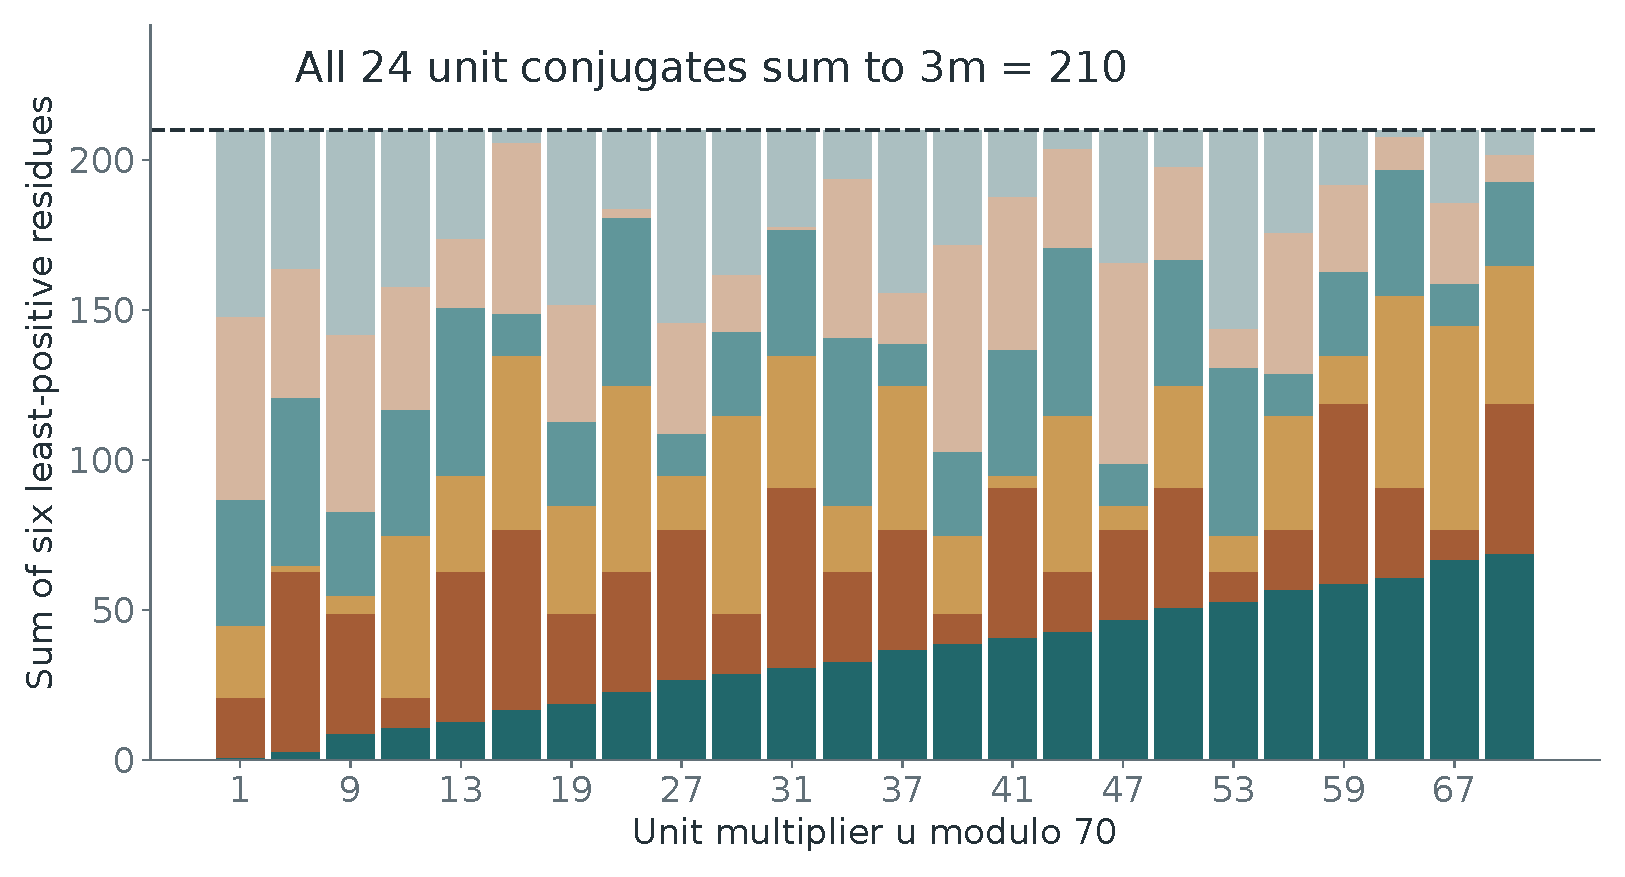
\includegraphics[width=0.98\linewidth]{11_balanced_orbit70.pdf}\caption{Every ordered unit conjugate of the named degree-70 character has sum 210. This exact example identifies Hodge type and does not itself construct a cycle.}\end{figure}

\chapter{Exact conductor polyphase}
For a packet \(a\), define
\[
g(a)=\gcd(m,a_0,\ldots,a_5),
\qquad
c(a)=\frac{m}{g(a)}.
\]
For a count vector, $L_k$ denotes scaling each residue entry by $k$ while multiplying the modulus by $k$. Writing \(a=g(a)b\), the coordinate-power map
\[
\pi_{g(a)}:X_m^4\longrightarrow X_{c(a)}^4,
\qquad [x_i]\longmapsto[x_i^{g(a)}],
\]
sends the degree-\(c(a)\) character packet \(b\) to the degree-\(m\) packet \(a\).

\begin{theorem}[Conductor descent]
Every imprimitive balanced packet at degree \(m\) is the coordinate-power pullback of a unique full-conductor packet at its exact conductor \(c\mid m\). Consequently
\[
\mathcal B_m=\bigsqcup_{c\mid m}L_{m/c}\mathcal B_c^{\mathrm{full}}.
\]
\end{theorem}
\begin{proof}
If every occupied residue is divisible by \(g\), divide the six entries and the modulus by \(g\). Since
\[
\langle ugb_i\rangle_{gc}=g\langle \bar u b_i\rangle_c,
\]
the balance equation descends. The maximal common divisor is unique. The converse follows by scaling.
\end{proof}

For \(d\mid m\), let
\[
E_{m,d}=\frac1{(m/d)^5}\pi_{m/d}^*\pi_{m/d*}.
\]
On a character of exact conductor \(c\),
\[
E_{m,d}=\begin{cases}1,&c\mid d,\\0,&c\nmid d.\end{cases}
\]
Therefore
\begin{equation}\label{eq:legacy-8.1}
\boxed{E_{m,d}E_{m,e}=E_{m,\gcd(d,e)}.}\end{equation}
M\"obius inversion produces pairwise orthogonal exact-conductor projectors
\begin{equation}\label{eq:legacy-8.2}
\boxed{
Q_{m,c}=\sum_{d\mid c}\mu(c/d)E_{m,d}.
}\end{equation}
They satisfy
\[
Q_{m,c}Q_{m,e}=\delta_{ce}Q_{m,c},
\qquad
\sum_{c\mid m}Q_{m,c}=I.
\]
Hence
\begin{equation}\label{eq:legacy-8.3}
\boxed{
H^4_{\mathrm{prim}}(X_m^4,\Q)
=\bigoplus_{c\mid m}\operatorname{im}Q_{m,c}.
}\end{equation}
Each \(Q_{m,c}\) is a rational linear combination of graph correspondences, so the conductor decomposition is itself algebraic.



\begin{figure}[tbp]\centering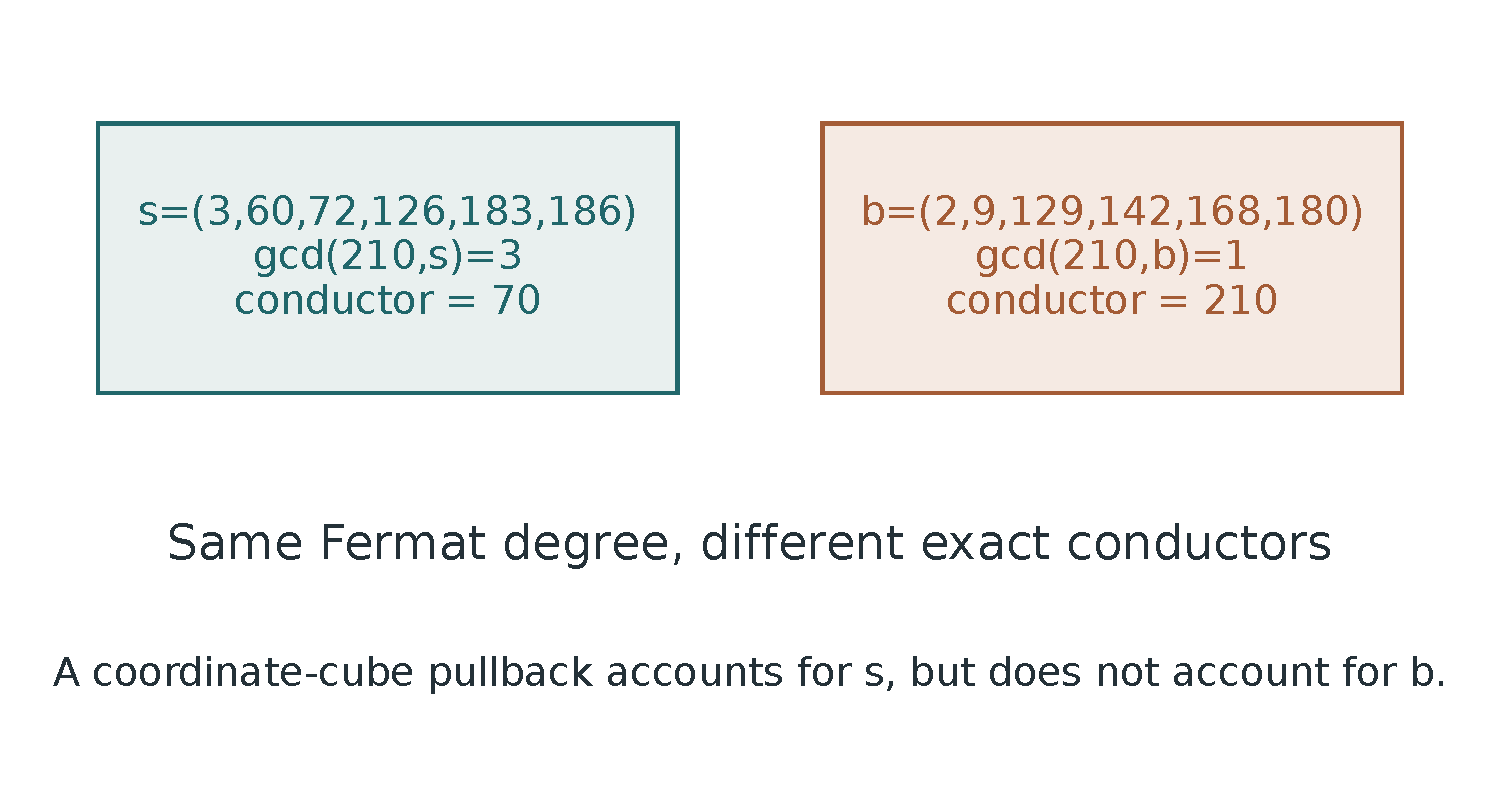
\includegraphics[width=0.98\linewidth]{12_conductor_descent.pdf}\caption{Exact conductor descent in the named example. Coordinate-power inflation enlarges the ambient degree while preserving the old conductor.}\end{figure}

\chapter{Algebraic certificate grammar}
Fix a full-conductor orbit in \(\mathcal B_m\). The constructive program tests a hierarchy of increasingly general certificate channels.

\section{Complementary pairs}
For \(1\le r<m\), let
\[
p_r=e_r+e_{m-r}.
\]
A packet is pair-decomposable when
\begin{equation}\label{eq:legacy-9.1}
n=p_{r_1}+p_{r_2}+p_{r_3}.\end{equation}
These are the standard linear-cycle or Tate-pair packets.

\section{Balanced four-packets and saturation}
Let
\[
\mathcal F_m=
\left\{
\gamma\in\mathbf N^{m-1}:
\mathbf1^T\gamma=4,
\quad R_m\gamma=2m\,\mathbf1
\right\}.
\]
A saturated certificate is an exact nonnegative identity
\begin{equation}\label{eq:legacy-9.2}
\boxed{
 n+\sum_{j=1}^{2N-3}p_{r_j}
 =\sum_{i=1}^N\gamma_i,
 \qquad \gamma_i\in\mathcal F_m.
}\end{equation}
The case \(N=2\) is one-step quasi-decomposition. Higher \(N\) allows several surface packets to reconstruct one six-packet after Tate stabilization.

The algebraic implication must use the actual classical correspondence operations. A balanced four-entry packet is algebraic by Lefschetz $(1,1)$ on a Fermat surface. Concatenate the $N$ surface characters using the Shioda--Ran construction, then remove precisely the $2N-3$ complementary pairs by the classical pair-removal theorem. The ambient dimension rises to $4N-2$ before cancellation. This proves algebraicity of a packet admitting such an identity once those cited operations and their character conventions have been checked. It does not authorize cancellation of arbitrary tensor factors. The August 15 status note correctly demanded a complete correspondence-level account of the proposed general grammar. The concrete degree-210 application below spells out the necessary stabilization and uses only the checked pair-removal theorem.

\section{Dual charges}
An antisymmetric charge is a rational function \(w\) on residues satisfying
\[
w(m-r)=-w(r)
\]
and
\[
\sum_r\gamma_r w(r)=0
\qquad\forall \gamma\in\mathcal F_m.
\]
Such a charge vanishes on every complementary pair and on every saturated identity. Writing $w(n)=\sum_r n_r w(r)$, if \(w(n)\ne0\), the entire lower-packet saturation semigroup is excluded. This is a universal obstruction to a grammar, not a nonalgebraicity theorem.

\section{Curve, Delsarte, and incidence channels}
A curve certificate splits the six entries into triples
\[
a=A\sqcup B,
\qquad \sum A=m,
\quad \sum B=2m,
\quad B=uA\pmod m.
\]
The resulting \((1,1)\) class on a product of Fermat curves is algebraic by Lefschetz \((1,1)\), and the join correspondence returns a surface class.

A Delsarte certificate consists of an exponent matrix and a resolved monomial map to a lower-degree hypersurface carrying an already algebraic packet. An incidence certificate uses algebraic lowering maps
\[
A_r:V\to H^2(Y_r)
\]
whose combined positive transfer
\[
T=\sum_rA_r^\dagger A_r
\]
is invertible on the packet. Divisor lowering and Cayley--Hamilton reconstruction then produce the cycle.

\chapter{The degree-33 rejection branch and its collapse}
The degree-33 Fermat fourfold provided a stringent test because one rational orbit escaped the ordinary decomposable and standard channels. A rejection attempt first isolated the packet, excluded several obvious cycle families, and then discovered a cross-family cubic correspondence that algebraizes it.

\section{The exceptional packet}
A representative is
\[
a=(7,10,13,19,22,28),
\]
or after permutation,
\[
\widetilde a=(7,19,28,10,13,22).
\]
Every unit conjugate has residue sum \(99=3\cdot33\), so the orbit is rational of type \((2,2)\). It is not totally pair-decomposable. The previously proposed symmetric surface
\[
W=\{p_1(x^{11})=p_2(x^{11})=p_3(x^{11})=0\}
\]
does not carry the primitive packet: Newton's identity makes the third equation redundant on \(X_{33}^4\), and
\[
[W]=242h^2.
\]
Thus \(W\) is purely ambient.

\section{Klein--Delsarte cubic}
Consider the smooth cubic fourfold
\[
Y:\quad y_0^2y_4+y_1^2y_0+y_2^2y_1+y_3^2y_2+y_4^2y_3+y_5^3=0.
\]
An explicit monomial exponent matrix gives a dominant rational map
\[
\phi:X_{33}^4\dashrightarrow Y
\]
whose projective-torus lattice map has Smith diagonal
\[
(1,33,33,33,33),
\]
so the generic torus degree is \(33^4\).

Take the cubic Jacobian-ring class
\[
P(y)=y_1y_2y_5.
\]
Its exponent vector is $b=(0,1,1,0,0,1)$. Write $C=33A^{-1}$ for the cubic exponent matrix $A$. The class is nonzero in the degree-three Jacobian ring. The residue pullback has the exact exponent identity
\begin{equation}\label{eq:legacy-10.1}
C^Tb+10\mathbf1=(6,18,27,9,12,21)=\widetilde a-\mathbf1.\end{equation}
Therefore the pullback of the corresponding primitive cubic \((2,2)\)-class lies in the one-dimensional Fermat line \(V(\widetilde a)\).

The Laurent exponent match is a useful exact certificate, but by itself it does not prove that a rational class lifts through a compact graph. A complete manuscript argument instead uses the torus-carrier criterion developed in Chapter~\ref{ch:carrier70}. For the reordered character, the exponent matrix $A$ of the cubic satisfies
\[
A^T\widetilde a/33=\beta=(1,2,2,1,1,2),\qquad C=33A^{-1}.
\]
With $r_0$ the first row of $A$, put $u=\beta-3r_0$. Then $\mathbf1^Tu=0$ and $C^Tu=\widetilde a-99e_0$. These identities establish triviality of the selected character on the torus deck group. Every selected character has full support, so its restriction to the coordinate torus is an isomorphism on the packet. Finite étale descent gives a pure rational weight-four Hodge substructure on the cubic torus. The lowest-weight image theorem and semisimplicity give a rational $(2,2)$ lift to the smooth cubic. Classical cubic algebraicity then supplies a surface class. Pull back through a resolved graph, apply the rational orbit projector, and use boundary injectivity to identify the returned class.

\begin{manuscriptclaim}[Degree-33 packet construction]
Subject to the resolved graph and the cited mixed-Hodge inputs in the preceding argument, the rational packet generated by $(7,10,13,19,22,28)$ is algebraic on $X_{33}^4$. The exponent identities are finite exact certificates. The compact geometric implication is a manuscript argument and is not certified by those identities alone.
\end{manuscriptclaim}



The episode is methodologically important. Failure of a finite cycle grammar is not evidence of nonalgebraicity. It may indicate a missing cross-family correspondence.

\begin{figure}[tbp]\centering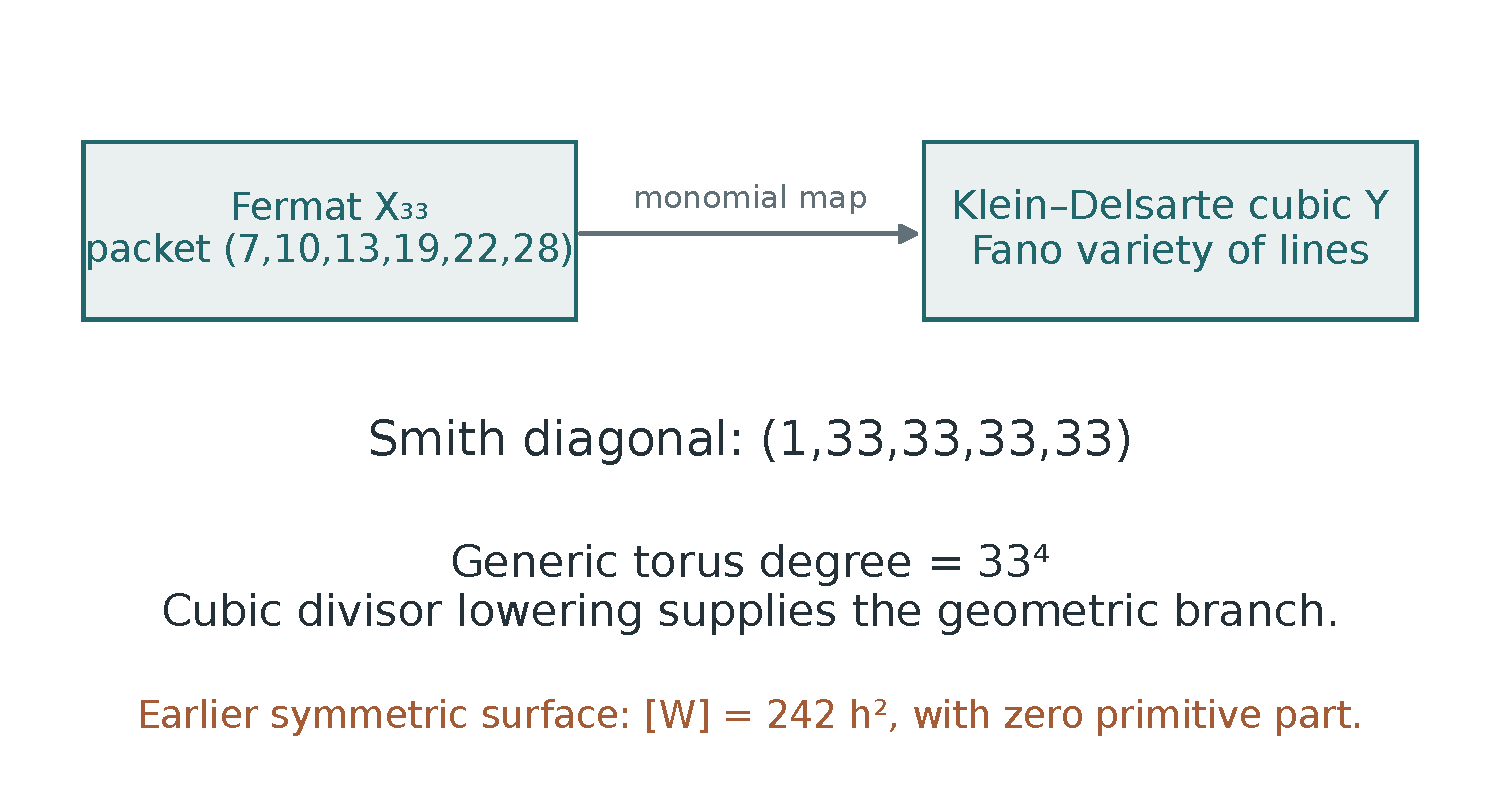
\includegraphics[width=0.98\linewidth]{15_klein33_route.pdf}\caption{The degree-33 torus/cubic construction requires deck invariance, full-support boundary control, a rational Hodge lift and the resolved algebraic graph.}\end{figure}

\chapter{Infinite towers and full-conductor promotion}
The coordinate-power maps propagate every solved seed through infinitely many degrees.

\begin{theorem}[Infinite packet tower]
Let \(W\) be an algebraic rational character packet on \(X_d^{2p}\). For every \(k\ge1\), its coordinate-power pullback is an algebraic packet on \(X_{kd}^{2p}\). Applied to the preceding degree-33 construction under its geometric hypotheses, this gives a 20-dimensional algebraic packet on every $X_{33k}^4$.
\end{theorem}

The tower packet remains an old conductor-33 sector. A stronger construction appends a complementary pair
\[
(1,m-1)
\]
after scaling a solved seed to modulus \(m=kd\). If
\[
b=(b_0,\ldots,b_{2p+1})
\]
is algebraic at degree \(d\), then
\[
\Theta_{m,b}=(kb_0,\ldots,kb_{2p+1},1,m-1)
\]
has full raw conductor \(m\) and middle Hodge type two dimensions higher. Its rational orbit has dimension \(\varphi(m)\). This produces full-raw-conductor algebraic packets of unbounded rank.

Raw conductor is not the complete novelty invariant: removing Tate pairs or reversing joins can reveal a smaller stable conductor. The stable residual should therefore be defined only after eliminating conductor descent, Tate suspension, joins, Delsarte pullbacks, and incidence channels.

\chapter{Prime-power classification}
The following manuscript classification uses a primitive-character filtration and a six-entry mass bound. At filtration level one the kernel-to-lower-level argument must be replaced by the base-prime Fourier argument stated below.

\section{Valuation strata and orbit mass}
Let \(m=p^r\) with \(p\) odd. Decompose the entries by exact \(p\)-adic valuation. At one stratum, write \(a=p^jb\), with \(b\in U_{p^{r-j}}\), and define the odd count
\[
\delta_j(b)=n_j(b)-n_j(-b).
\]
Since the packet has six entries,
\begin{equation}\label{eq:legacy-12.1}
\|\delta_j\|_1\le 12.\end{equation}
For $s\ge2$, primitive odd characters force \(\delta_j\) to be constant on the kernel cosets of
\[
U_{p^s}\to U_{p^{s-1}}.
\]
A nonzero odd kernel-orbit defect has mass at least \(2p\).

At $s=1$, all odd characters modulo $p$ are primitive. Their sawtooth Fourier coefficients are nonzero, so the odd count vector has every Fourier coefficient zero and is zero. This gives complementary pairing at the base prime level. The higher-level mass argument applies only for $s\ge2$. The needed odd-character nonvanishing is a classical analytic leaf, checked through Sharifi's cyclotomic-field notes \cite{SharifiDirichlet}.

\section{Large odd primes}
If \(p\ge7\), then \(2p>12\), so every odd defect vanishes. Each residue occurs with the same multiplicity as its complement. Therefore every packet is three complementary pairs.

\section{The three-primary branch}
For $p=3$ and $r\ge2$, a higher-level kernel orbit has three elements. Define
\[
O_b=\{b,b+q,b+2q\},
\qquad q=3^{r-1},
\]
and
\[
\Gamma_b=O_b\sqcup\{3(q-b)\}.
\]
Take $1\le b<q$ with $3\nmid b$, ensuring all entries are nonzero. Then \(\Gamma_b\) is a balanced four-packet. A case analysis on the number of oriented kernel orbits gives exact identities expressing every full-conductor nonpair packet as a pair/surface packet or a one-step saturated sum of two balanced four-packets.

\section{The five-primary branch}
For $p=5$ and $r\ge2$, a nonzero odd defect consumes exactly five unit entries. The base case $r=1$ was already handled by the base-prime Fourier argument. The sixth entry is forced by balance. Up to the unit action there is one full-conductor exceptional orbit
\begin{equation}\label{eq:legacy-12.2}
\boxed{
\alpha_{5^r}=
(1,1+q,1+2q,1+3q,1+4q,5q-5),
\qquad q=5^{r-1}.
}\end{equation}
All other packets lie in the pair/surface grammar. The family \eqref{eq:legacy-12.2} is the pure five-primary Hasse--Davenport branch.



\begin{center}
\small
\begin{tabular}{rrrr}\toprule $m$ & Full orbits & Pair/SAT(2) & Residual \\
\midrule
49 & 124 & 124 & 0 \\
81 & 436 & 436 & 0 \\
125 & 827 & 826 pair & 1 \\
\bottomrule\end{tabular}

\end{center}

\chapter{Weighted dyadic reconstruction}
Prime \(2\) cannot be handled by inserting \(p=2\) into the odd-prime orbit-mass proof. The unit group has the separate form
\[
\mathbf Z_2^\times\cong\{\pm1\}\times(1+4\mathbf Z_2).
\]
The first address is a sign packet, only afterward does the principal-unit refinement begin.

Let $s\ge3$, \(m=2^s\), \(h=2^{s-1}\), and write $\rho_s=\rho_{2^s}$. For an odd residue \(b\pmod h\), its two lifts are \(b\) and \(b+h\). Define
\[
L_sn(b)=n(b)+n(b+h),
\qquad
D_sn(b)=n(b)-n(b+h).
\]
For every odd unit \(u\), one has the exact weighted identity
\begin{equation}\label{eq:legacy-13.1}
\boxed{
\begin{aligned}
&n(b)\rho_s(ub)+n(b+h)\rho_s(u(b+h))\\
&\qquad=L_sn(b)\rho_{s-1}(\bar ub)
+2^{s-2}D_sn(b)\varepsilon_s(u,b),
\end{aligned}
}\end{equation}
where \(\varepsilon_s(u,b)\in\{\pm1\}\). Repetition yields a Haar-like expansion whose detail packets carry visible powers of two. The Hodge balance equation becomes a binary carry relation between weighted details.



Exact enumeration gives:
\begin{center}
\small
\begin{tabular}{rrrrrr}\toprule $m$ & Full orbits & Pair & SAT(2) & SAT(3) & Unresolved \\
\midrule
8 & 13 & 9 & 4 & 0 & 0 \\
16 & 45 & 27 & 18 & 0 & 0 \\
32 & 134 & 91 & 42 & 1 & 0 \\
64 & 419 & 331 & 87 & 1 & 0 \\
128 & 1435 & 1259 & 175 & 1 & 0 \\
\bottomrule\end{tabular}

\end{center}
The table suggests one residual orbit beginning at \(m=32\). The remaining derivation proposes an all-degree explanation. Its uniform status was downgraded by the later August 15 note, so this edition preserves the argument as a manuscript claim requiring a complete audit.

\begin{figure}[tbp]\centering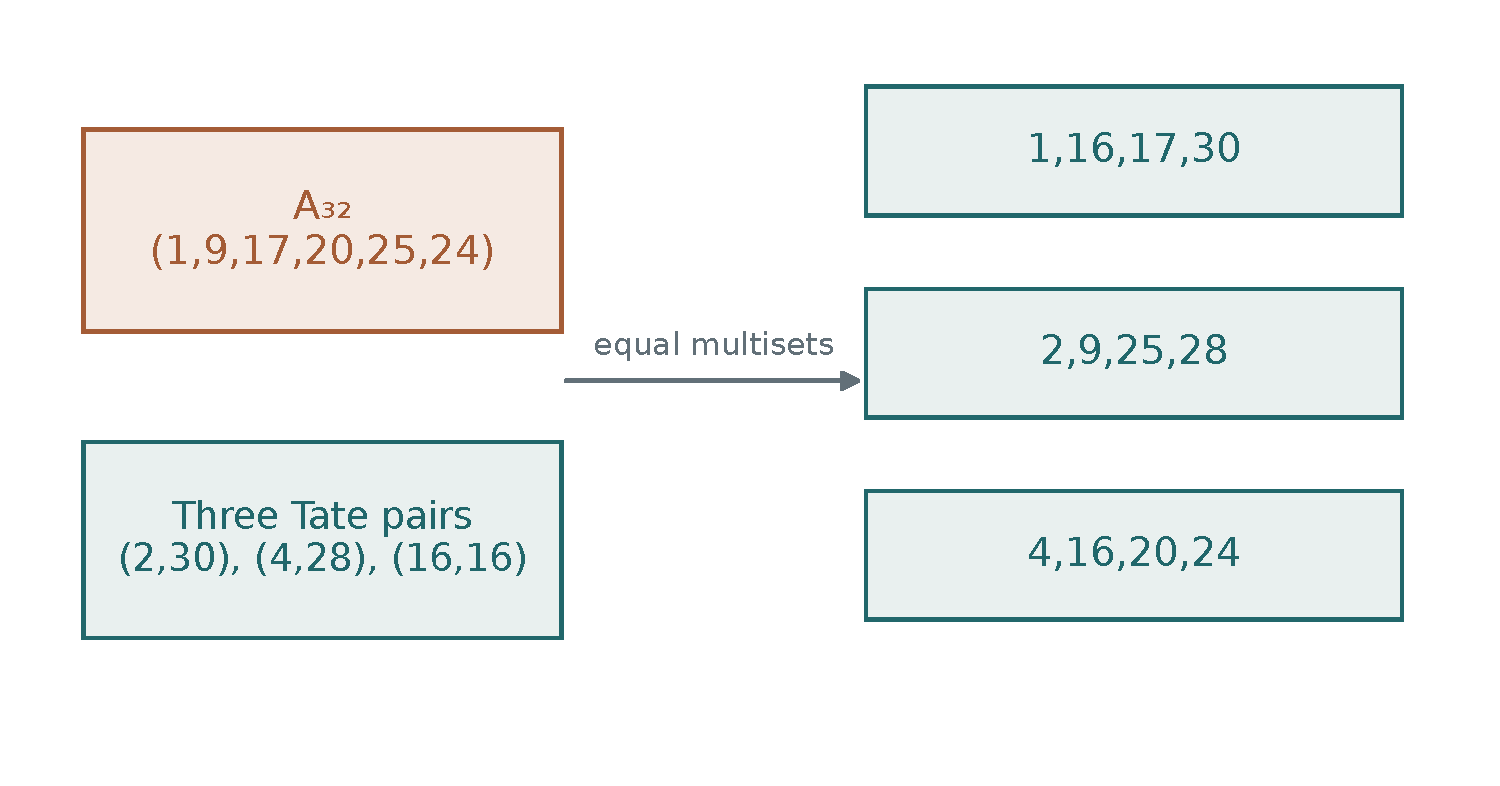
\includegraphics[width=0.98\linewidth]{13_dyadic_sat3.pdf}\caption{The three finite dyadic representatives have exact SAT(3) identities. These identities do not prove all-degree grammar coverage.}\end{figure}

\section{Complement defects and dyadic triangles}
Put
\[
q=\frac m4,
\qquad h=2q,
\qquad m=4q.
\]
For a packet count vector \(n\), define its oriented complement defect
\[
\partial n=\sum_{r=1}^{h-1}d_n(r)[r],
\qquad
d_n(r)=n_r-n_{m-r}.
\]
The self-complementary residue \(h\) contributes zero. Since
\(\rho_m(m-r)=-\rho_m(r)\), the balanced-packet equation is equivalent to
\[
\sum_{r=1}^{h-1}d_n(r)\rho_m(ur)=0
\qquad\text{for every odd unit }u.
\]
Moreover,
\[
\|\partial n\|_1=\sum_{r=1}^{h-1}|d_n(r)|\le 6.
\]
Thus the dyadic problem is a short-vector problem in an integral defect lattice.

For \(1\le b<q\), define the triangle defect
\[
\kappa_b=[2b]-[b]+[h-b].
\]
It is realized by the four-packet
\[
\Gamma_b=(2b,h-b,h,m-b).
\]

\begin{manuscriptclaim}[Dyadic triangle relation]
For every odd unit \(u\) and every \(1\le b<q\),
\[
\rho_m(2ub)-\rho_m(ub)+\rho_m(u(h-b))=0.
\]
Consequently \(\kappa_b\) is balanced and \(\Gamma_b\in\mathcal F_m\).
\end{manuscriptclaim}
\begin{proof}
Let \(x=\langle ub\rangle_m\). If \(0<x<h\), then
\[
\rho_m(2x)=2x-h,
\qquad
\rho_m(x)=x-h,
\qquad
\rho_m(h-x)=-x.
\]
Their indicated combination is zero. If \(h<x<m\), write \(x=m-y\) with \(0<y<h\), then
\[
\rho_m(2x)=h-2y,
\qquad
\rho_m(x)=h-y,
\qquad
\rho_m(h-x)=y,
\]
and the same cancellation occurs. Since \(u\) is odd, \(uh\equiv h\pmod m\), so \(u(h-b)\equiv h-ub\pmod m\). This proves the identity.
\end{proof}

\begin{figure}[tbp]\centering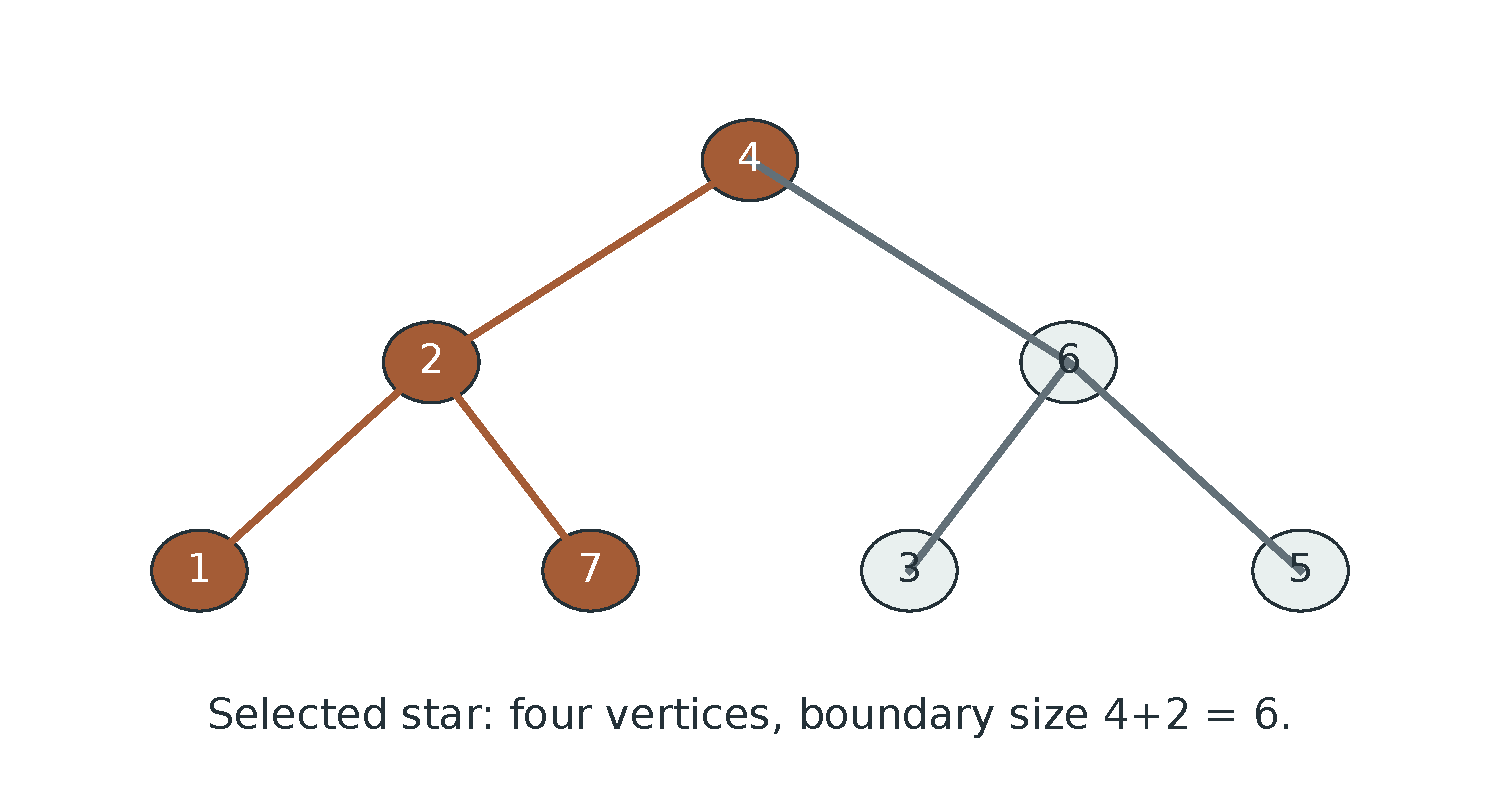
\includegraphics[width=0.98\linewidth]{14_dyadic_tree32.pdf}\caption{The finite degree-32 defect tree. The proposed uniform derivation is retained separately with its publication-status boundary.}\end{figure}

\section{The integral triangle basis}
Let
\[
\mathcal K_m=
\left\{
 d\in\mathbf Z^{h-1}:
 \sum_{r=1}^{h-1}d(r)\rho_m(ur)=0
 \text{ for every odd }u
\right\}.
\]
The triangle relations do not merely generate examples, they form the whole balanced defect lattice.

\begin{manuscriptclaim}[Integral dyadic triangle basis]
For \(m=2^s\), \(s\ge3\), the vectors
\[
\{\kappa_b:1\le b<q\}
\]
form a \(\mathbf Z\)-basis of \(\mathcal K_m\).
\end{manuscriptclaim}
\begin{proof}
Set \(r_0=q/2\). On the vertex set
\[
V_m=\{1,2,\ldots,q-1\},
\]
define, for \(b\ne r_0\),
\[
p(b)=
\begin{cases}
2b,&b<r_0,\\
2(q-b),&b>r_0,
\end{cases}
\qquad
\epsilon_b=
\begin{cases}
+1,&b<r_0,\\
-1,&b>r_0.
\end{cases}
\]
The map \(p\) raises the two-adic valuation by one, so repeated application reaches \(r_0\). It therefore defines a rooted tree.

Suppose \(d=\sum_{b=1}^{q-1}z_b\kappa_b\). Its even coordinates are
\[
d(q)=z_{r_0},
\qquad
d(2b)=z_b-\epsilon_bz_{p(b)}
\quad(b\ne r_0).
\]
Starting at the root and moving toward the leaves, these equations recover every \(z_b\) integrally. Hence the triangle vectors are linearly independent and their even-coordinate map is unimodular.

Now take \(d\in\mathcal K_m\), recover the unique integers \(z_b\) from its even coordinates, and subtract \(\sum_bz_b\kappa_b\). The residual balanced vector is supported only on the odd residues \(1\le r<h\). The corresponding square sawtooth matrix is nonsingular. Indeed, extend an odd-support vector to an odd function on \(U_m\). Convolution with \(\rho_m\) is diagonalized by the odd Dirichlet characters, with eigenvalues
\[
\lambda_\chi=
\sum_{a\in U_m}\rho_m(a)\overline{\chi(a)}
=
\sum_{a\in U_m}a\overline{\chi(a)}.
\]
If \(\chi\) is induced from a primitive odd character \(\chi^*\) of conductor \(2^t\), then
\[
\lambda_{\chi,2^s}=2^{s-t}\lambda_{\chi^*,2^t}.
\]
The primitive value is, up to a nonzero scalar, the generalized Bernoulli value \(B_{1,\overline{\chi^*}}\), equivalently \(-L(0,\overline{\chi^*})\), and is nonzero for every odd primitive character \cite{WashingtonCyclotomic,SharifiDirichlet}. Thus every odd Fourier eigenvalue is nonzero. The odd residual must vanish, so the \(\kappa_b\) span \(\mathcal K_m\) over \(\mathbf Z\).
\end{proof}

\section{The trivalent defect tree}
The integral basis turns defect mass into exact tree variation. Define a sign gauge by
\[
\tau_{r_0}=1,
\qquad
\tau_b=\epsilon_b\tau_{p(b)},
\qquad
y_b=\tau_bz_b.
\]
Attach one zero-valued boundary leaf to the root and two zero-valued boundary leaves to every odd vertex. Every vertex of the resulting augmented tree \(\widetilde T_m\) has degree three. The boundary edges correspond bijectively to defect coordinates: the root edge is labelled \(q\), the edge from \(b\) to \(p(b)\) is labelled \(2b\), and the two leaves at an odd \(b\) are labelled \(b\) and \(h-b\).

\begin{manuscriptclaim}[Exact trivalent-tree norm]
If \(d=\sum_bz_b\kappa_b\in\mathcal K_m\), then
\begin{equation}\label{eq:legacy-13.2}
\boxed{
\|d\|_1
=|y_{r_0}|
+\sum_{b\ne r_0}|y_b-y_{p(b)}|
+2\sum_{\substack{1\le b<q\\ b\text{ odd}}}|y_b|.
}\end{equation}
The right side is the total variation of the integer function \(y\) on \(\widetilde T_m\) with zero boundary values.
\end{manuscriptclaim}
\begin{proof}
The root coordinate is \(d(q)=z_{r_0}\). For \(b\ne r_0\), multiplying
\(d(2b)=z_b-\epsilon_bz_{p(b)}\) by \(\tau_b\) gives
\[
\tau_bd(2b)=y_b-y_{p(b)}.
\]
For odd \(b\), the two odd coordinates are
\[
d(b)=-z_b,
\qquad
d(h-b)=z_b.
\]
Taking absolute values and summing all defect coordinates gives \eqref{eq:legacy-13.2}.
\end{proof}

For an integer-valued \(y\), discrete coarea gives
\begin{equation}\label{eq:legacy-13.3}
\operatorname{TV}(y)
=
\sum_{k\ge1}|\partial\{y\ge k\}|
+
\sum_{k\ge1}|\partial\{y\le-k\}|.\end{equation}
If \(S\) is a finite forest of internal vertices of a trivalent tree and \(c(S)\) is its number of connected components, then
\begin{equation}\label{eq:legacy-13.4}
|\partial S|=|S|+2c(S),\end{equation}
because \(3|S|=2(|S|-c(S))+|\partial S|\).

\begin{manuscriptclaim}[All defect shapes of mass at most six]
Let \(d\in\mathcal K_m\) satisfy \(\|d\|_1\le6\), and let \(y\) be its gauged coefficient function. Exactly one of the following occurs:
\begin{enumerate}
\item \(y=0\)
\item \(y=\pm2\) at one vertex and is zero elsewhere
\item \(y\) has two singleton components, each with value \(\pm1\)
\item \(y=\pm1\) on one connected subtree containing at most four vertices and is zero elsewhere.
\end{enumerate}
For a balanced four-packet, only the zero shape, a single vertex, or one tree edge can occur.
\end{manuscriptclaim}
\begin{proof}
Apply \eqref{eq:legacy-13.3}--\eqref{eq:legacy-13.4}. A nonempty level-set component with \(k\) vertices costs \(k+2\). If \(|y|\ge2\), two nonempty nested level sets already cost at least six, equality forces both to be the same singleton. If positive and negative values both occur, their first level sets cost at least three each, equality forces two singleton components. Otherwise \(y\) has one sign, and a connected support of size \(k\) costs \(k+2\), so \(k\le4\). Two same-sign components can have total cost at most six only when both are singletons. Replacing six by four leaves only a vertex or an edge.
\end{proof}

\section{SAT(2) closure and the four-star obstruction}
For a defect \(d\), let \(\operatorname{red}(d)\) be the unmatched residue multiset: a positive coefficient at \(r\) contributes copies of \(r\), while a negative coefficient contributes copies of \(m-r\). Its length is \(\|d\|_1\). Every packet with defect \(d\) is \(\operatorname{red}(d)\) together with complementary pairs and copies of \(h\).

A one-vertex tree atom has defect \(\pm\kappa_b\) after the gauge sign and is represented by \(\Gamma_b\) or its conjugate, its reduced length is three and its fourth entry is \(h\). A one-edge atom has defect mass four, so its reduced multiset itself is a balanced four-packet. A zero atom is any union of two complementary pairs.

\begin{manuscriptclaim}[Exact SAT(2) criterion]
Let \(n\) be a balanced six-packet at modulus \(m=2^s\). Then \(n\) is pair-decomposable or has an SAT(2) certificate unless its gauged defect is \(\pm1\) on a four-vertex star \(K_{1,3}\) in the internal tree \(T_m\). A four-star has no SAT(2) certificate.
\end{manuscriptclaim}
\begin{proof}
Every nonstar shape in the preceding proposition splits into at most two four-packet atoms:
\begin{itemize}
\item a vertex or edge is paired with a zero atom
\item a three-vertex path is an edge plus its remaining terminal vertex
\item a four-vertex path is the union of two disjoint edges
\item a doubled singleton is two copies of one vertex atom
\item two singleton components are the corresponding two vertex atoms.
\end{itemize}
These defect splittings lift to exact nonnegative multiset identities. For a vertex, the neutral remainder of the six-packet is \(h\) plus one complementary pair, for an edge it is one complementary pair. A zero four-packet absorbs that pair and the stabilizing pair. Cutting a three- or four-vertex path produces exactly one oppositely oriented boundary edge, hence exactly one complementary pair in the union of the two atom packets, this is the SAT(2) stabilizer. In the three-vertex case, the vertex atom also supplies the unique neutral \(h\). For two vertex atoms, their two neutral entries are \((h,h)=p_h\). The zero-defect case is already a union of three complementary pairs. Thus in every nonstar case there are \(\gamma_1,\gamma_2\in\mathcal F_m\) and a complementary pair \(p_r\) such that
\[
n+p_r=\gamma_1+\gamma_2.
\]

Conversely, suppose a four-star defect had an SAT(2) certificate. Each balanced four-packet has tree support equal to zero, one vertex, or one edge. The sum of two such supports must produce four nonzero star vertices. Therefore both supports must be disjoint edges covering all four vertices. This would be a perfect matching of \(K_{1,3}\), which does not exist. Hence the star is the unique tree obstruction to SAT(2).
\end{proof}

\section{Conductor of a star and its unique unit orbit}
The tree also determines exactly when the star obstruction has full conductor.

\begin{manuscriptclaim}[Star conductor]
Let a four-star have center \(c\), and write \(j=v_2(c)\). The gcd of \(m\) with its six packet entries is
\[
2^{j-1}.
\]
Hence a star has full conductor exactly when \(v_2(c)=1\).
\end{manuscriptclaim}
\begin{proof}
Use the boundary-edge labels of \(\widetilde T_m\). The two children of \(c\) have valuation \(j-1\). The four boundary edges leaving those children have labels of exact valuation \(j-1\): for \(j=1\) they are the odd leaf labels, and for \(j>1\) they are labels \(2b\) coming from grandchildren of valuation \(j-2\). The two boundary edges leaving the parent side have larger valuation. Thus every nonzero defect coordinate is divisible by \(2^{j-1}\), and at least four have exact valuation \(j-1\). Replacing a defect coordinate \(r\) by the packet entry \(m-r\) does not change its two-adic valuation. The stated gcd follows.
\end{proof}

Assume now \(s\ge5\) and let a full-conductor star have center \(c=2a\) with \(a\) odd. Up to global conjugation, expanding its four triangle atoms gives the unordered packet
\begin{equation}\label{eq:legacy-13.5}
P_a=
(8a,q-a,2q-a,2q-4a,3q-a,4q-a).\end{equation}
The cases \(c<q/2\) and \(c>q/2\) give the same unordered tuple after the internal-edge cancellations. Choose an odd \(u\) satisfying
\[
ua\equiv1\pmod{2q}.
\]
Since \(uq\equiv q\) or \(3q\pmod{4q}\), multiplication by \(u\) sends \eqref{eq:legacy-13.5} to
\[
P_1=(8,q-1,2q-4,2q-1,3q-1,4q-1).
\]
Its conjugate is
\begin{equation}\label{eq:legacy-13.6}
\boxed{
A_m=
\left(
1,\frac m4+1,\frac m2+1,\frac m2+4,
\frac{3m}4+1,m-8
\right).
}\end{equation}
Thus every full-conductor star belongs to one \(U_m\)-orbit.

The packet \(A_m\) obeys the exact uniform SAT(3) identity
\begin{equation}\label{eq:legacy-13.7}
\begin{aligned}
&A_m+(2,m-2)+(4,m-4)+(m/2,m/2)\\
&=(1,m/2,m/2+1,m-2)\\
&\quad +(2,m/4+1,3m/4+1,m-4)\\
&\quad +(4,m/2,m/2+4,m-8).
\end{aligned}\end{equation}
The first and third packets on the right have defects \(-\kappa_1\) and \(-\kappa_4\). The middle packet has defect \(-\kappa_2+\kappa_{q-1}\), an edge atom. Hence all three are balanced four-packets, and \eqref{eq:legacy-13.7} is an identity of multisets.

\begin{manuscriptclaim}[All-degree dyadic uniqueness]
Let \(m=2^s\), \(s\ge3\). Every full-conductor balanced six-packet is pair-decomposable or SAT(2), except that for \(s\ge5\) there is exactly one residual unit orbit, represented by \(A_m\). This orbit is SAT(3) by \eqref{eq:legacy-13.7}. For \(m=8\) and \(m=16\), no four-star exists and there is no residual orbit.
\end{manuscriptclaim}
\begin{proof}
The trivalent-tree norm and coarea classification list every defect of mass at most six. The SAT(2) criterion closes every listed shape except a four-star. The star-conductor lemma forces a full-conductor star center to have valuation one, and the calculation \eqref{eq:legacy-13.5}--\eqref{eq:legacy-13.6} places all such stars in the single orbit of \(A_m\). The trees for \(m=8\) and \(m=16\) have no internal vertex with three internal neighbors. Finally, \eqref{eq:legacy-13.7} closes the unique residual orbit at saturation depth three.
\end{proof}

\begin{manuscriptclaim}[Complete dyadic grammar]
After exact conductor descent, every balanced packet at every dyadic modulus is generated by complementary pairs, SAT(2) surface packets, and coordinate-power pullbacks of the single SAT(3) family \(A_{2^t}\). No second residual dyadic family occurs at any depth.
\end{manuscriptclaim}

\begin{resultbox}[Uniform dyadic status]
The August 6 manuscript called uniform uniqueness closed. The August 15 status note restored it to a uniform write-up obligation. The proposed proof uses an integral triangle basis, an exact total-variation model, discrete coarea, and star conductor. This edition does not reverse the later downgrade on the strength of finite agreement.
\end{resultbox}

The archived companion dyadic verification report records complete orbit counts through $m=128$ and structural identities through $2^{14}$. The October replay freshly reconstructs the complete census through 128 and the triangle/tree identities through $2^9$. The report file is preserved evidence, rather than an executable verifier or a current replay of the larger historical range. These computations support the finite identities. They do not supply a current independent proof of the all-degree claim.

\chapter{Finite global audit through degree 100}
The finite audit exactly enumerates balanced packets, reduces them by unit orbits, checks pair and SAT(2) certificates, and searches higher saturated identities with \(N\le8\). Every returned identity is rechecked by exact integer arithmetic.

The archived named verification groups report the following outcomes:
\begin{center}
\small
\begin{tabular}{lrr}\toprule Suite & Passed & Total \\
\midrule
projector resolved hodge calculus & 18 & 18 \\
fermat33 klein closure & 14 & 14 \\
infinite klein tower & 4 & 4 \\
conductor polyphase & 4 & 4 \\
odd prime power audit & 13 & 13 \\
\midrule Total & 53 & 53 \\
\bottomrule\end{tabular}

\end{center}
The archived dyadic report records \(89{,}478{,}480\) coefficient checks through \(2^{14}\). The October replay independently checked 87,376 coefficients for exponents $3\le s\le9$. The larger historical count was not rerun in full. The archived packet audit reports completeness through degree \(100\) for its implemented grammar, which is not a completeness theorem for all correspondence channels.

After removing the degree-33 Klein channel and the degree-39 curve channel, every remaining post-saturation degree in the audit is divisible by five. This is a powerful localization of the residual grammar, but it is not by itself a universal proof.



\section{Exact residual representatives}
\small
\begin{longtable}{rp{0.68\textwidth}}\toprule Degree & Post-saturation representatives \\
\midrule\endfirsthead
\toprule Degree & Post-saturation representatives \\
\midrule\endhead
25 & \texttt{(1,6,11,16,20,21)} \\
33 & \texttt{(1,4,16,22,25,31)} \\
35 & \texttt{(1,8,15,22,29,30)} \\
39 & \texttt{(1,7,16,22,34,37)} \\
40 & \texttt{(1,9,17,25,33,35)} \\
45 & \texttt{(1,10,19,28,37,40); (1,19,20,28,30,37)} \\
50 & \texttt{(1,7,27,30,41,44); (1,11,21,31,41,45); (1,13,22,32,40,42)} \\
55 & \texttt{(1,12,23,34,45,50)} \\
65 & \texttt{(1,14,27,40,53,60)} \\
70 & \texttt{(1,6,43,45,57,58); (1,15,29,43,57,65); (1,20,24,42,61,62); (1,20,29,43,57,60); (1,29,35,43,45,57)} \\
75 & \texttt{(1,16,31,46,61,70)} \\
80 & \texttt{(1,17,33,49,65,75)} \\
85 & \texttt{(1,18,35,52,69,80)} \\
90 & \texttt{(1,8,26,62,85,88); (1,19,37,55,73,85); (1,19,37,60,73,80); (1,19,37,65,73,75); (1,23,38,55,74,79); (1,38,46,55,56,74); (2,38,45,55,56,74)} \\
95 & \texttt{(1,20,39,58,77,90)} \\
100 & \texttt{(1,21,41,61,81,95)} \\
\bottomrule\end{longtable}

\normalsize

The residuals are not random. Their mod-5 phase profiles form a small local grammar.

\compactpart{Part VIII. CRT--Kummer Polyphase and the Imaginary CM Half-Twist}

\chapter{Local mod-5 phase grammar}
Assume \(m=5q\) and first suppose \((5,q)=1\). For \(b\pmod q\) and a phase \(r\in\{0,1,2,3,4\}\), let \(\lambda_r(b)\) be the CRT lift satisfying
\[
\lambda_r(b)\equiv r\pmod5,
\qquad
\lambda_r(b)\equiv b\pmod q.
\]
The finite audit reveals four canonical multiplicity profiles, up to multiplication by a unit modulo five:
\[
(1,0,0,0,5),
\quad
(2,1,1,1,1),
\quad
(1,0,2,1,2),
\quad
(1,0,1,3,1).
\]
The first is the complete-five-phase K5 packet, the second is a four-phase K4 lift, and the final two are one K23 pair--triple mechanism.



\section{K4 four-phase reduction}
Choose nonzero residues \(b,c,d\pmod q\) and put
\[
e\equiv-5^{-1}b\pmod q.
\]
Define
\[
A_{b,c,d}=
(\lambda_1(b),\lambda_2(b),\lambda_3(b),\lambda_4(b),5c,5d)
\]
and
\[
\Gamma_{b,c,d}=(b,c,d,e).
\]

\begin{theorem}[Four-phase CRT reduction]
The six-packet \(A_{b,c,d}\) is balanced modulo \(5q\) if and only if the four-packet \(\Gamma_{b,c,d}\) is balanced modulo \(q\).
\end{theorem}
\begin{proof}
For a unit \(u\), let \(s=\langle ub\rangle_q\) and \(z=\langle u5^{-1}b\rangle_q\). The complete five-element fiber over \(s\) has sum \(5s+10q\), its phase-zero lift is \(5z\). The four nonzero phases therefore sum to \(5s+10q-5z\). Adding the last two entries and imposing the middle value \(15q\) gives
\[
s+\langle uc\rangle_q+\langle ud\rangle_q-z=q.
\]
Since \(\langle ue\rangle_q=q-z\), this is exactly the balance equation for \((b,c,d,e)\).
\end{proof}

All 16 audited K4 residuals reduce exactly to balanced four-packets.

\chapter{K23 pair--triple factorization}
Let a K23 packet have one phase-zero entry and five nonzero phases:
\[
A=P\sqcup T\sqcup\{5e\},
\qquad |P|=2,
\quad |T|=3,
\]
with
\[
\sum P\equiv0\pmod5,
\qquad
\sum T\equiv0\pmod5.
\]
Write
\[
\sum P=5C,
\qquad
\sum T=5D,
\]
and reduce \(C,D\) modulo \(q\) to representatives \(c,d\). Require $c,d,e$ to be nonzero modulo $q$ so that all three resulting character blocks have full support. Degenerate cases must leave this construction and be handled through pair removal or another channel. For example $(1,14,2,9,14,5)$ at modulus 15 is balanced and admits the indicated phase split, but $P=(1,14)$ gives $c=0$. The phase condition alone is insufficient. Define
\[
C_P=P\sqcup\{m-5c\},
\]
\[
S_T=T\sqcup\{m-5d\},
\]
and
\[
L=(5c,5d,5e).
\]

For any nonzero-entry block $B$ at modulus $m$, put $h_B(u)=m^{-1}\sum_{r\in B}\langle ur\rangle_m$, with multiplicities retained.

\begin{theorem}[Exact K23 packet identity]
One has the exact multiset equality
\begin{equation}\label{eq:legacy-15.1}
\boxed{
A+(5c,m-5c)+(5d,m-5d)=C_P+S_T+L.
}\end{equation}
For every unit \(u\pmod m\),
\[
h_{C_P}(u)+h_{S_T}(u)+h_L(u)=5,
\]
and \(c+d+e\equiv0\pmod q\).
\end{theorem}

The five nonzero phases have only two irreducible possibilities: all five phases are equal, or they contain a complementary pair and a zero-sum triple. Indeed, if no complementary phase pair occurs, the phase support lies in one of four two-element subsets, the zero-sum condition forces all five entries to use one phase. This proves the local K5/K23 dichotomy.



After fixing a common cyclotomic coefficient field and a diagonal character projector, write the selected factor schematically as
\[
N=e_{\mathrm{diag}}\bigl(M(C_P)\otimes M(S_T)\bigr).
\]
An ordinary tensor product of rational packets contains off-diagonal embedding pairs and is generally not rank one. Rank one here refers only to a selected eigenspace after scalar extension. The coefficient field and projector are part of the unresolved correspondence specification.
The Hodge-level identity implies that \(N(1)\) has weight one and has Hodge type opposite to the lower curve packet \(M(L)\) at every embedding.

\begin{figure}[tbp]\centering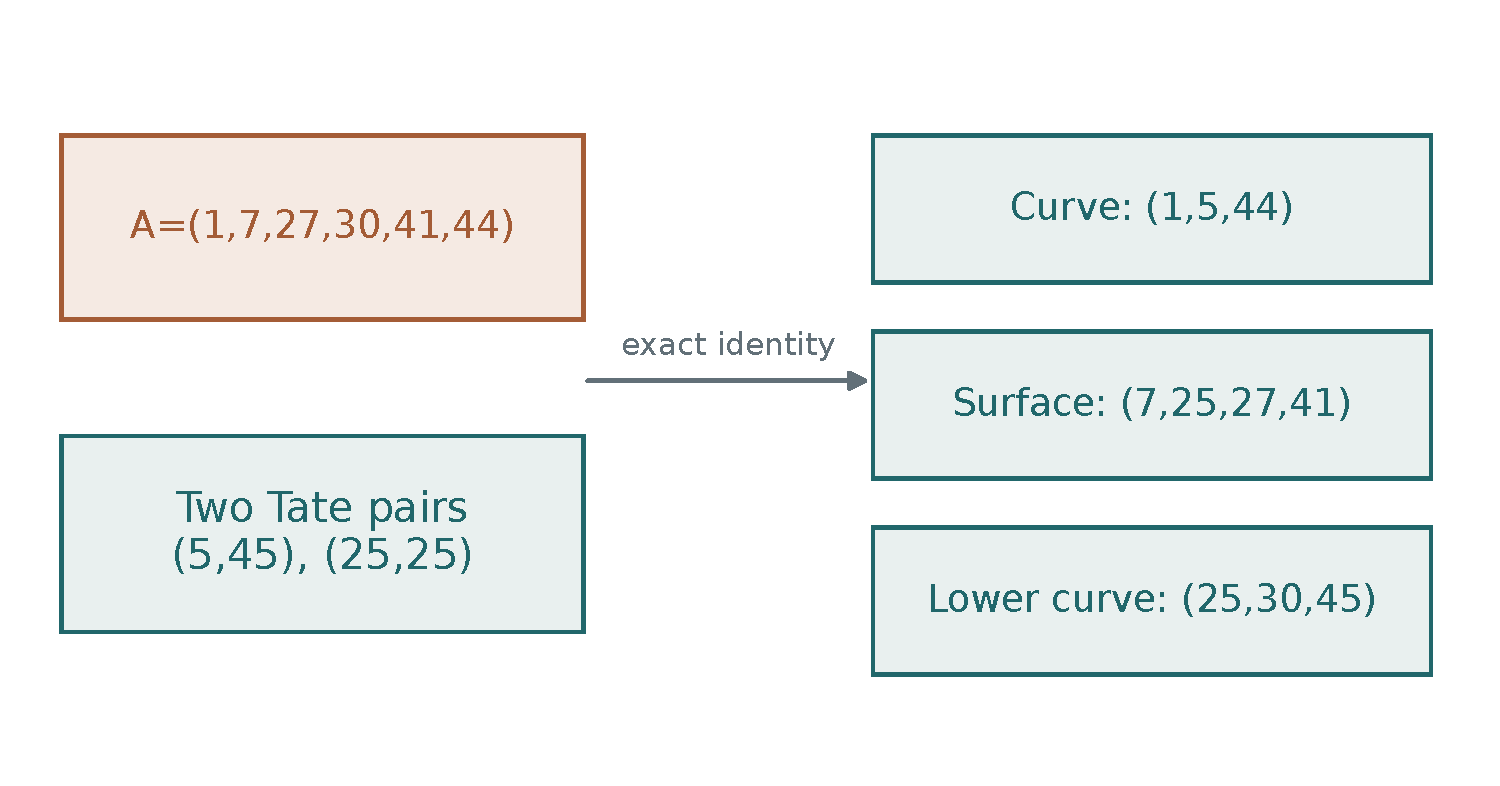
\includegraphics[width=0.98\linewidth]{16_k23_factorization50.pdf}\caption{A valid finite K23 factorization at modulus 50, with all required character entries nonzero.}\end{figure}

\chapter{Imaginary CM selector}
Write the lower curve packet as
\[
\ell=(c,d,e)\pmod q,
\qquad c+d+e\equiv0\pmod q.
\]
Let \(K=\Q(\zeta_q)\) and define
\begin{equation}\label{eq:legacy-16.1}
\boxed{
\Delta_\ell=(1-\zeta_q^c)(1-\zeta_q^d)(1-\zeta_q^e).
}\end{equation}

\begin{theorem}[Pure imaginary selector]
\[
\overline{\Delta_\ell}=-\Delta_\ell.
\]
\end{theorem}
\begin{proof}
Since
\[
1-\zeta_q^{-a}=-\zeta_q^{-a}(1-\zeta_q^a),
\]
complex conjugation multiplies the product by
\[
(-1)^3\zeta_q^{-(c+d+e)}=-1.
\]
\end{proof}

For an embedding \(\sigma_u:\zeta_q\mapsto\zeta_q^u\), let
\[
h_\ell(u)=\frac{\langle uc\rangle_q+\langle ud\rangle_q+\langle ue\rangle_q}{q}\in\{1,2\}.
\]
Using
\[
1-e^{2\pi ir/q}=-2i\,e^{\pi ir/q}\sin\frac{\pi r}{q},
\]
one obtains
\begin{equation}\label{eq:legacy-16.2}
\sigma_u(\Delta_\ell)
=8i(-1)^{h_\ell(u)}
\prod_{j=1}^3
\sin\frac{\pi\langle u\ell_j\rangle_q}{q}.\end{equation}
Here $(\ell_1,\ell_2,\ell_3)=(c,d,e)$ is an indexed triple, so repeated residues contribute repeated factors. Every sine factor is positive, so the sign of the imaginary part is exactly the Hodge sign. Consequently the CM type of \(N(1)\) is the conjugate of the CM type of the lower curve packet:
\begin{equation}\label{eq:legacy-16.3}
\boxed{
\Sigma_N=\overline{\Sigma_\ell}.
}\end{equation}
This is the rigorous form of the statement that the half-twist occurs on the imaginary plane.



The exact audit generates 364 K23 certificates from seven rational packet orbits. Every certificate obeys the opposite curve CM sign, factors through a lower conductor, and is a Galois translate of an upper-half-plane CM type.

\begin{center}
\small
\begin{tabular}{lr}\toprule Item & Value \\
\midrule
K23 rational orbits & 7 \\
Exact K23 certificates & 364 \\
Opposite curve CM sign & True \\
Lower-conductor factorization & True \\
Upper-half-plane CM translate & True \\
\bottomrule\end{tabular}

\end{center}

In the audited cases, the minimal CM conductors are \(3,5,7,\) or \(9\), even when the original fourfold modulus is \(50,70,\) or \(90\). Thus the weight-one carrier is not arbitrary: it is a character factor of the Jacobian of a lower-degree Fermat curve.

\begin{figure}[tbp]\centering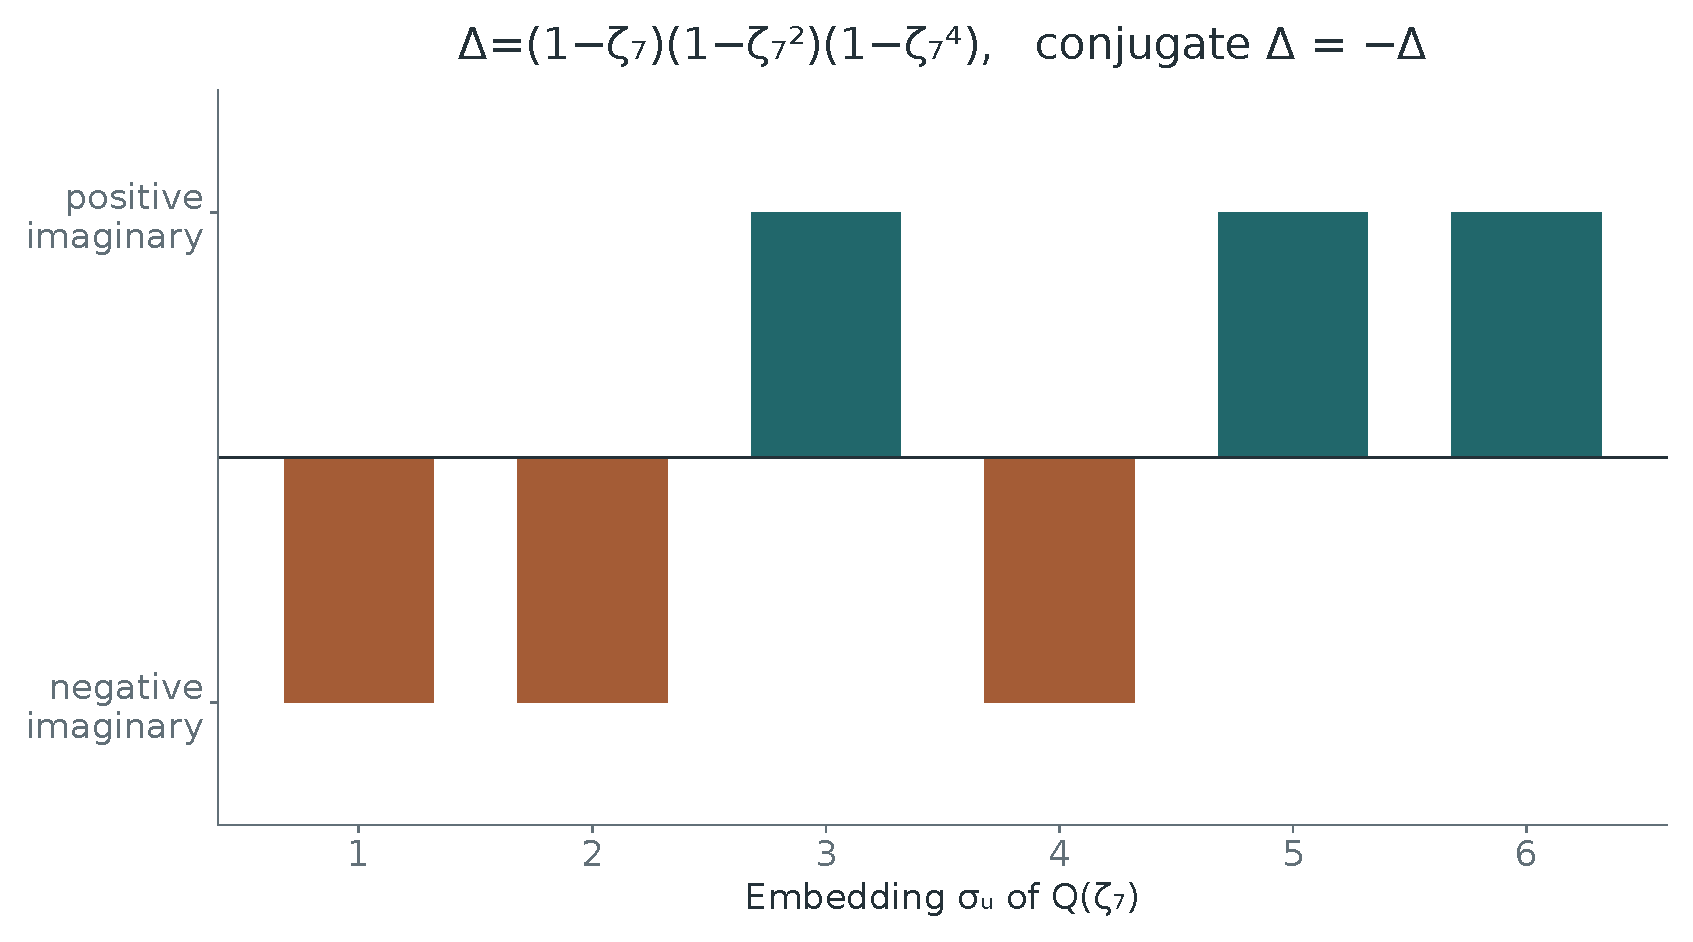
\includegraphics[width=0.98\linewidth]{17_cm_imaginary_sign.pdf}\caption{The exact imaginary selector sign in a retained example. Matching signs does not construct a rational Chow correspondence.}\end{figure}

\chapter{Explicit carrier and remaining Chow map}
For an audited CM type, the lower Fermat curve provides a candidate rational character-orbit factor of its Jacobian. Write $e_{\mathrm{orb}}J(F_d)$ for that factor, up to isogeny. The idempotent selects the complete rational Galois orbit. A projector onto just one holomorphic CM half-plane would not be rational and is not an algebraic rational packet projector.

The desired correspondence is schematically
\[
\Gamma\in\CH^{\ast}(F_d\times C_P\times S_T)_{\Q},\qquad
\Gamma_*:e_{\mathrm{orb}}H^1(F_d)\longrightarrow
e_{\mathrm{diag}}\bigl(M(C_P)\otimes M(S_T)\bigr)(1).
\]
This formula is a target specification, not a constructed map. Its coefficient field, diagonal projector, rational multiplicities, and dimensions must be fixed before an isomorphism can be asserted. The smaller CM conductor can have a smaller rational degree than the original packet. Matching sign functions alone does not resolve that difference.

After the typing has been supplied, a nonzero equivariant map between corresponding rank-one eigenspaces is an isomorphism over the splitting field. Proving that the map is induced by an algebraic correspondence remains essential. One needs a Kummer or half-twist correspondence with the correct covariance and a nonzero period or intersection coefficient. Tensoring a verified map with the conjugate lower curve packet can then place a class in divisor degree on a product of curves or abelian varieties. Lefschetz $(1,1)$ and actual Fermat join maps would transport it back.

\begin{openproblem}[Typed CM packet correspondence]
Specify the fields, projectors and rational multiplicities, construct the algebraic map, and prove its nonzero character coefficient. The 364 audited sign certificates identify candidate factors. They do not solve this problem. The finite-field Chow-motive constructions of Otsubo and Yamazaki provide related context, and are not a characteristic-zero correspondence proof for these packets \cite{OtsuboYamazaki}.
\end{openproblem}

\begin{figure}[tbp]\centering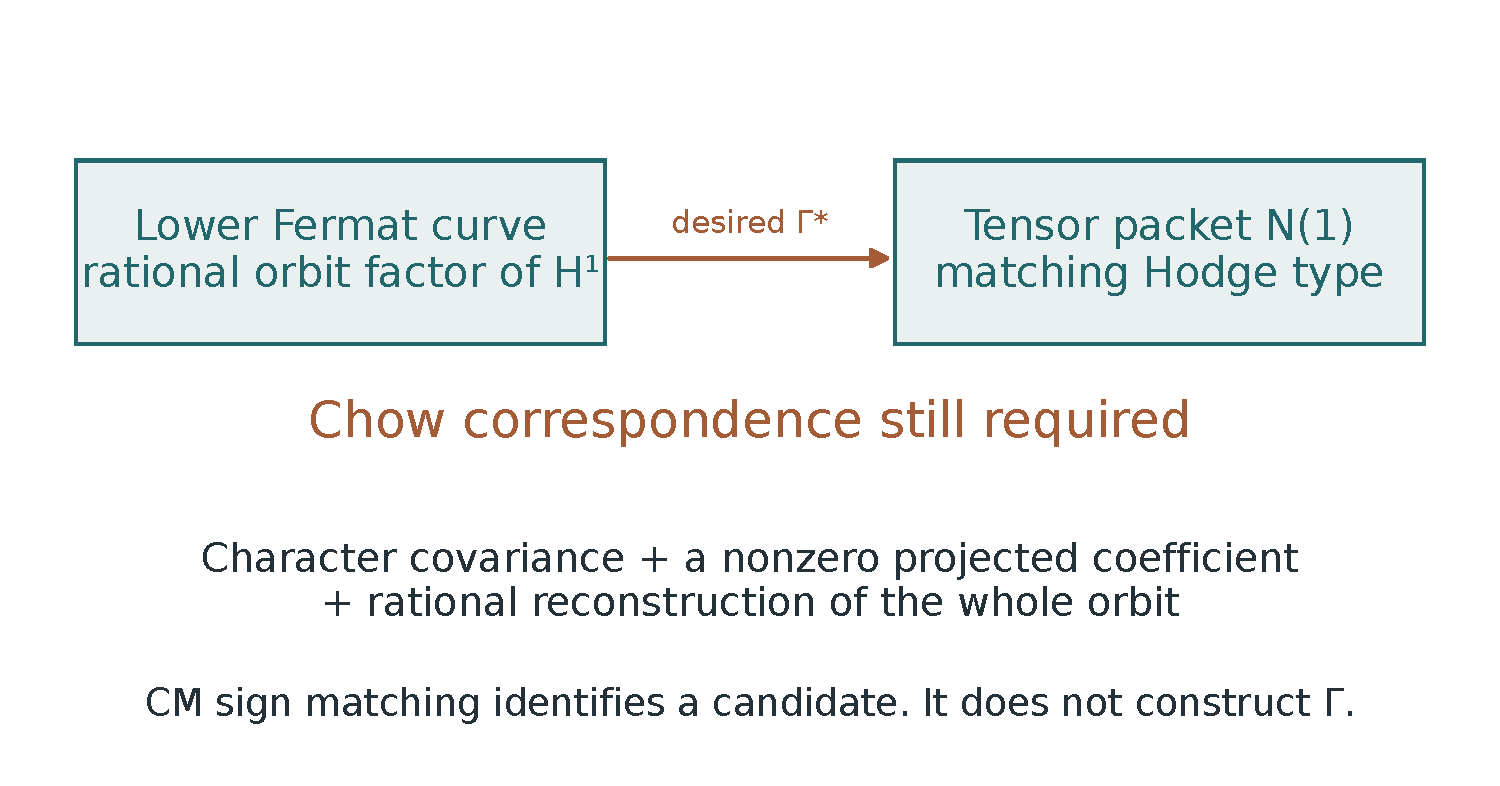
\includegraphics[width=0.98\linewidth]{18_missing_chow_bridge.pdf}\caption{The typed algebraic CM bridge is an open construction. Coefficient field, projectors, multiplicities and nonzero period are part of the target.}\end{figure}

\chapter{Correct literature and novelty map}
Kang is cited in the checked later literature for the all-degree Fermat-fourfold Hodge result, while its original exact theorem and proof were not extracted here \cite{KangFermat}. Separately, da Silva studies which packets are generated by Shioda-style induced-cycle criteria and records the degree-$33$ failure of that criterion \cite{DaSilvaFermat}. The October source contracts authenticate the Kang attribution through the checked later literature while recording that its original proof was not extracted. No historical priority claim is made for this constructive program.

The constructive contribution of the packet program is therefore not best described as the first proof of the rational Hodge conjecture for all Fermat fourfolds. Its strongest defensible targets are:
\begin{itemize}
\item explicit conductor projectors as algebraic correspondences
\item an algorithmic packet certificate grammar
\item a worked cross-family Klein--Delsarte construction at degree 33
\item infinite conductor towers and full-raw-conductor promotions
\item odd prime-power packet classifications
\item a weighted dyadic recursion and a proposed all-degree classification with one SAT(3) orbit
\item exact CRT--Kummer reductions for K4 and K23 packets
\item an imaginary CM selector and explicit lower Fermat-curve carriers
\item an explicit packet-resolved Chow correspondence algorithm
\end{itemize}

\begin{resultbox}[Constructive status]
The abstract existence question for Fermat fourfolds is treated as prior published work. The packet program supplies a detailed constructive architecture and several explicit manuscript correspondence constructions, without a historical novelty claim. Universal constructive coverage also requires a complete mixed-conductor grammar. The typed CM correspondence is one focused gap inside that larger problem.
\end{resultbox}

\compactpart{Part IX. Verification, Audit, and Final Constructive Theorem}

\chapter{Verification ledger}
The complete edition separates symbolic theorems, finite exact checks, geometric correspondences, and literature claims.

\section{Finite checks}
The original Hodge-calculus release passed 18 finite checks. The archived Fermat extension reports the following historical checks, whose fresh replay ranges are distinguished in the current evidence chapter:
\begin{itemize}
\item 14 exact degree-33 Klein checks
\item 4 infinite tower checks
\item 4 exact conductor-polyphase checks
\item 13 odd prime-power checks
\item 89,478,480 dyadic weighted coefficient identities
\item exact packet classifications at dyadic degrees through 128
\item an independent trivalent-tree/SAT(2) audit and structural dyadic checks through $2^{14}$
\item exact balanced-packet audit through degree 100
\item 364 K23 CM-type certificates
\end{itemize}

\section{What finite checks establish}
They establish exact arithmetic identities, matrix products, orbit counts, conductor decompositions, Hodge balance, and nonnegative multiset equalities for every tested instance. They also detect false universal conjectures quickly. The proposed dyadic uniqueness statement is not inferred from these checks. Its manuscript derivation is preserved with the later uniform-write-up downgrade.

\section{What finite checks do not establish}
They do not replace:
\begin{itemize}
\item a universal mixed-prime phase-classification proof beyond the audited range
\item a Chow-level Kummer--Schur or half-twist correspondence
\item a historical priority audit
\end{itemize}

\chapter{Final theorem stack}
The constructive Fermat program can be stated as a dependency stack.

\begin{theorem}[Conditional explicit packet theorem]
Fix a packet that is admitted by the implemented certificate grammar. Assume the following correspondence statements for its chosen channel:
\begin{enumerate}
\item saturated Fermat joins are associative on Chow motives and complementary Tate factors cancel
\item every Delsarte torus map used by the certificate grammar extends through a resolved graph with full-support boundary annihilation
\item every K5, K4, and K23 packet used by the chosen certificate has its correctly typed Chow correspondence with a proved nonzero character coefficient
\end{enumerate}
Then that packet has an explicit packet-resolved algebraic cycle representative. A conclusion for every Fermat fourfold packet additionally requires universal mixed-conductor coverage by this grammar, which has not been proved here.
\end{theorem}
\begin{proof}
Apply the exact conductor projectors. Descend each nonzero component to its full-conductor seed. Use the supplied grammar certificate for the seed, whether pair, saturation, curve, Delsarte, dyadic, or a Kummer phase channel. Use the corresponding Chow map to produce a nonzero cycle projection. Pull old packets back to the original degree and sum the orthogonal conductor components. Finally use the rational orbit projector or rational group-module reconstruction. A bare sum of all complex conjugate eigenvectors may vanish and is not a substitute for that rational construction.
\end{proof}

\begin{openproblem}[Unconditional constructive completion]
Write the missing correspondence maps explicitly and verify their nonzero packet matrix coefficients. A concentrated target is the correctly typed CM correspondence specified above. Universal mixed-conductor coverage is a separate obligation.
\end{openproblem}

\chapter{Research checklist}
\begin{longtable}{p{0.42\textwidth}p{0.17\textwidth}p{0.32\textwidth}}
\toprule
Task & Status & Required proof object \\
\midrule\endfirsthead
\toprule
Task & Status & Required proof object \\
\midrule\endhead
Universal balanced packet equation & Complete & Finite residue matrix \\
Exact conductor descent & Complete & Coordinate-power graph \\
M\"obius conductor projectors & Complete & Rational graph combination \\
Degree-33 Klein packet & Manuscript-level complete & Resolved graph and residue pullback \\
Infinite old-packet towers & Complete & Pullback/pushforward identity \\
Odd prime-power classification & Symbolically complete & Primitive-character filtration \\
Dyadic finite identities & Replayed in a bounded range & Weighted coefficient identities and finite tree data \\
K4 CRT reduction & Complete & Lower balanced four-packet \\
K23 local phase reduction & Audited instances & Pair--triple identity with nonzero-entry conditions \\
K23 CM sign descent & Complete & Imaginary selector $\Delta_\ell$ \\
Explicit lower CM carrier & Identified & Fermat-curve character idempotent \\
CM carrier Chow map & Open & Nonzero algebraic correspondence \\
All-degree constructive algorithm & Open & Universal coverage plus all required correspondence maps \\
Historical priority map & Open audit & Compare existence and constructive literature \\
\bottomrule
\end{longtable}

\chapter{Complete-edition conclusion}
The projector-resolved approach transforms the Hodge problem into a hierarchy of exact finite packets and explicit geometric transfers. For arbitrary varieties, the master obstruction remains the Hodge packet not occupied by algebraic-cycle channels. For Fermat fourfolds, diagonal symmetry makes every stage concrete: balanced residue equations, conductor projectors, prime-local refinements, nonnegative packet identities, and rank-one character motives.

The degree-33 rejection attempt illustrates the central lesson. A packet may evade every obvious lower-packet construction and still be algebraic through a hidden cross-family correspondence. A completed Klein--Delsarte correspondence supplies a seed for infinite conductor towers. The odd prime-power manuscript classification and the proposed dyadic tree derivation explain why local primes require distinct packet grammars. The audited mixed-prime residuals display a small Kummer phase system, without a proof that these patterns exhaust arbitrary conductors. Finally, the imaginary CM selector identifies the precise upper/lower embedding split and reduces the unknown weight-one carrier to a small Fermat-curve Jacobian factor.

The constructive endpoint is now sharply defined:
\begin{resultbox}[Final constructive endpoint]
Construct a correctly typed nonzero equivariant Chow correspondence for each admitted CM packet, and separately prove universal coverage of the certificate grammar.
\end{resultbox}
This task is narrower than the original conjecture and stronger than a numerical packet classification. It asks for an algorithmic cycle formula that exposes exactly how a Hodge packet becomes algebraic.



\compactpart{Part X. Geometric carriers and signed transfers}
\hypertarget{carrier70-a-normal-weighted-carrier-at-degree-70}{%
\chapter{A normal weighted carrier at degree
70}\label{ch:carrier70}\label{carrier70-a-normal-weighted-carrier-at-degree-70}}

The September 21 construction, reconciled with the October exact replay
and source audit.

\textbf{Status:} Manuscript-level special-case proof, with a separately
replayable exact algebraic certificate. The geometric proof remains at
manuscript level. The October review separately replayed the exact
algebra and checked the stated classical leaves. This is not a formal
verification of the geometry. This note does not prove the general Hodge
conjecture, does not cover every degree-70 packet, and makes no
historical novelty claim.

\hypertarget{carrier70-precise-statement}{%
\section{Precise statement}\label{carrier70-precise-statement}}

Write

\[
X_m=\{x_0^m+\cdots+x_5^m=0\}\subset\mathbf P^5_\mathbf C.
\]

The diagonal group is \(G_m=(\mu_m)^6/\mu_m\). For a character
\(a=(a_0,\ldots,a_5)\) with all entries nonzero modulo \(m\) and sum
zero modulo \(m\), let \(W_{[a]}\) denote the rational character-orbit
summand of primitive \(H^4(X_m,\mathbf Q)\).

\textbf{Proposition.} For

\[
m=70,\qquad a=(1,20,24,42,61,62),
\]

all classes in the 24-dimensional rational space \(W_{[a]}\) are
rational linear combinations of classes of algebraic surfaces on
\(X_{70}\). For every positive integer \(k\), the corresponding
pulled-back packet \(W_{[ka]}\) on \(X_{70k}\) is also algebraic.

The proof below uses the established rational Hodge theorem for smooth
projective uniruled fourfolds. It constructs the carrier and the
monomial correspondence explicitly. It does \textbf{not} list equations
for a basis of the surfaces supplied by that theorem.

\hypertarget{carrier70-hodge-type-of-the-packet}{%
\section{Hodge type of the packet}\label{carrier70-hodge-type-of-the-packet}}

The primitive Fermat eigenspaces for full-support characters are
one-dimensional over the splitting field. The Griffiths residue
description assigns type \((2,2)\) when the least-positive residues have
sum \(3m\). A rational orbit is of type \((2,2)\) precisely when this
holds for all its unit conjugates.

For every \(t\in(\mathbf Z/70\mathbf Z)^\times\), exact enumeration
gives

\[
\sum_{i=0}^{5}\langle ta_i\rangle_{70}=210.
\]

There are 24 conjugates, all distinct because \(a_0=1\). Thus the entire
rational orbit, not just a single complex residue vector, has type
\((2,2)\). The verifier stores every conjugate. The distinction between
a complex residue vector and a rational Hodge class is essential here.

The standard residue basis follows from Griffiths' description, a modern
source with the formula is Villaflor Loyola, \emph{Small codimension
components of the Hodge locus containing the Fermat variety},
arXiv:2001.01019, Section 1. For Fermat, the basis monomials diagonalize
the group action, giving the character description used here.

\hypertarget{carrier70-the-exact-carrier}{%
\section{The exact carrier}\label{carrier70-the-exact-carrier}}

Let

\[
A=\begin{pmatrix}
0&0&2&0&0&3\\
0&0&1&2&7&0\\
1&0&2&2&0&1\\
0&5&0&0&0&0\\
0&0&0&2&0&3\\
3&0&0&0&0&0
\end{pmatrix}.
\]

Rows are monomial exponents, columns correspond to \(y_0,\ldots,y_5\).
Direct rational arithmetic gives

\[
\det A=-2100,\qquad
A^{-1}\mathbf1=(1/3,1/5,1/10,1/10,1/10,4/15),
\]

\[
\mathbf1^TA^{-1}\mathbf1=11/10.
\]

Set \(W=(10,6,3,3,3,8)\) and \(D=30\), so \(AW=D\mathbf1\). Define

\[
Y=\{F=0\}\subset\mathbf P(10,6,3,3,3,8),
\]

\[
F=y_0^3+y_1^5+y_2^2y_5^3+y_2y_3^2y_4^7
  +y_0y_2^2y_3^2y_5+y_3^2y_5^3.
\]

Every monomial has weighted degree 30. The adjunction coefficient is

\[
D-\sum W_i=30-33=-3.
\]

This model is singular and is not quasismooth. The argument therefore
cannot invoke a quasismooth residue theorem or assume that its
resolution is Fano. Normality and uniruledness are proved separately
below.

\begin{figure}[tbp]\centering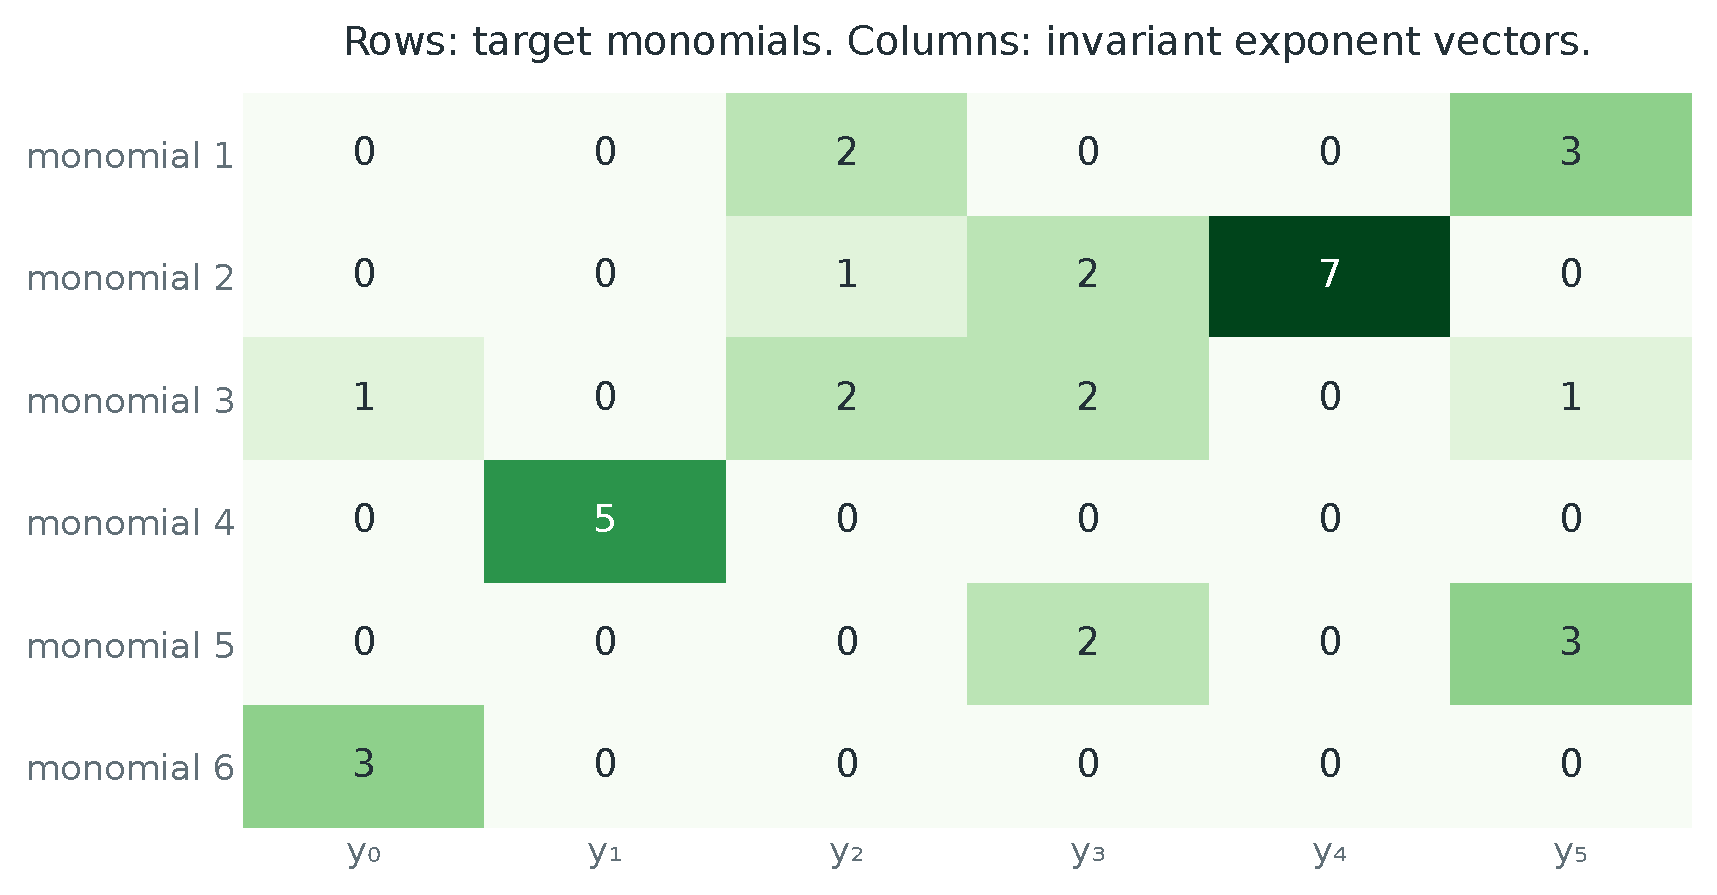
\includegraphics[width=0.98\linewidth]{19_carrier70_matrix.pdf}\caption{The exact exponent matrix. Rows are monomials and columns are target coordinates.}\end{figure}

\hypertarget{carrier70-an-explicit-finite-cover-on-the-tori}{%
\section{An explicit finite cover on the
tori}\label{carrier70-an-explicit-finite-cover-on-the-tori}}

Let \(M=210\), \(\alpha=3a\), and

\[
B=210A^{-1}=\begin{pmatrix}
0&0&0&0&0&70\\
0&0&0&42&0&0\\
42&0&63&0&-63&-21\\
-63&0&63&0&42&-21\\
12&30&-27&0&-3&9\\
42&0&-42&0&42&14
\end{pmatrix}.
\]

Then

\[
AB=210I,\qquad B\mathbf1=7W.
\]

On the projective tori define \(y_i=\prod_jx_j^{B_{ij}}\). Negative
exponents are allowed there. The second identity makes this well-defined
into the weighted projective torus, the first gives

\[
F(y(x))=x_0^{210}+\cdots+x_5^{210}.
\]

The induced map of five-dimensional tori is an isogeny. Consequently its
restriction is a finite étale cover

\[
q:U_{210}\longrightarrow U_Y,
\]

where \(U_{210}=X_{210}\cap\{\prod x_i\ne0\}\) and
\(U_Y=Y\cap\{\prod y_i\ne0\}\).

The target torus hypersurface is smooth because its finite étale
pullback is smooth. It is irreducible because its Laurent polynomial
pulls back under an injective full-rank monomial substitution to an
irreducible Fermat Laurent polynomial. Non-monomial factors remain
non-monomial under this substitution. The polynomial \(F\) has no
coordinate factor, so its projective closure \(Y\) is also irreducible.

\begin{figure}[tbp]\centering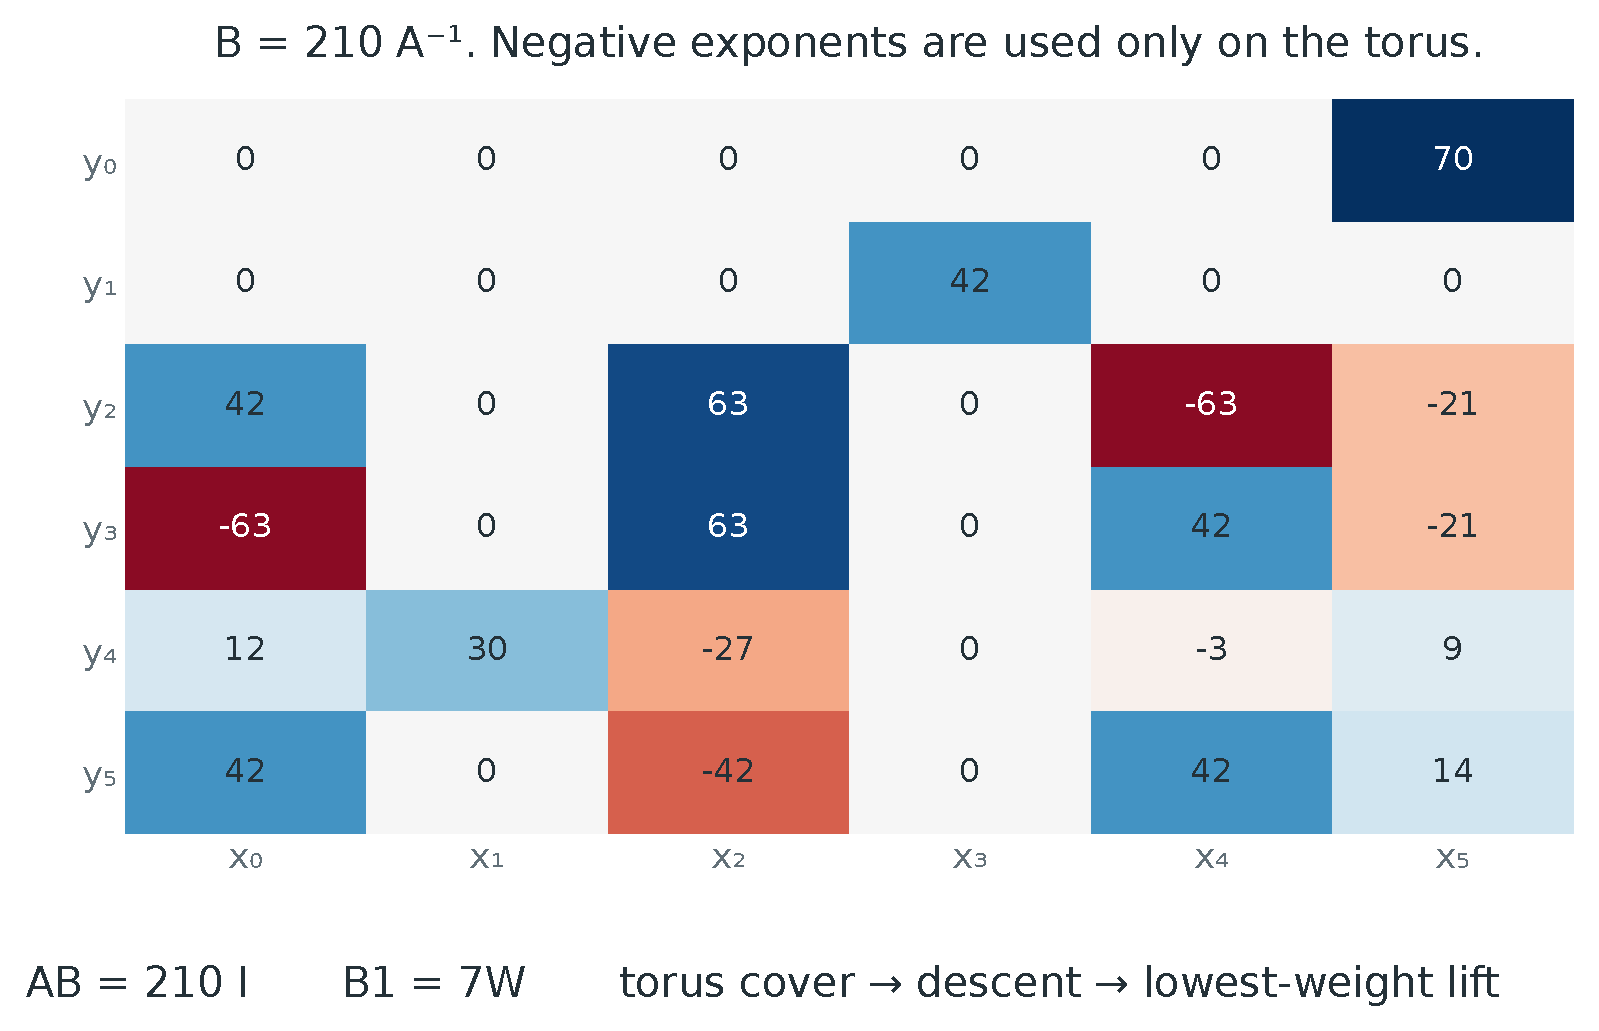
\includegraphics[width=0.98\linewidth]{22_carrier70_torus_matrix.pdf}\caption{The exact Laurent exponent matrix, with negative entries permitted on the torus.}\end{figure}

\hypertarget{carrier70-normality-and-the-canonical-class}{%
\section{Normality and the canonical
class}\label{carrier70-normality-and-the-canonical-class}}

Put \((u,v,s,t,c,z)=(y_0,y_1,y_2,y_3,y_4,y_5)\), so

\[
F=u^3+v^5+z^3(s^2+t^2)+st^2c^7+us^2t^2z.
\]

Its gradient is

\[
\begin{aligned}
F_u&=3u^2+s^2t^2z, &F_v&=5v^4,\\
F_s&=2sz^3+t^2c^7+2ust^2z,
&F_t&=2t(z^3+sc^7+us^2z),\\
F_c&=7st^2c^6,
&F_z&=3z^2(s^2+t^2)+us^2t^2.
\end{aligned}
\]

The cone singular locus is exactly

\[
\{y_0=y_1=y_2=y_3=0\}
\ \cup\ \{y_0=y_1=y_3=y_5=0\}
\ \cup\ \{y_0=y_1=y_4=y_5=0\}.
\]

Here is a direct verification of exhaustion. At a singular point,
\(v=0\) and \(st^2c^6=0\). The cases \(s=0\) or \(t=0\) give the
displayed planes immediately from the other derivatives. In the
remaining case \(s,t\ne0\), one has \(c=0\). If \(z=0\), then \(u=0\),
giving the third plane. If \(z\ne0\), the equations \(F_s=F_t=0\) give

\[
z^2+ut^2=z^2+us^2=0.
\]

Hence \(s^2=t^2=R\ne0\) and \(u=-z^2/R\). But then \(F_z=5Rz^2\ne0\), a
contradiction.

There is also an independent exact ideal certificate. For the gradient
ideal \(J\), the verifier proves

\[
\sqrt J=(y_0,y_1,y_2y_5,y_3y_4,y_3y_5).
\]

It checks that the gradient vanishes on the three planes and that the
powers

\[
y_0^3,\quad y_1^4,\quad (y_2y_5)^3,\quad
(y_3y_4)^{13},\quad (y_3y_5)^3
\]

belong to \(J\) by Gröbner reduction over \(\mathbf Q\). The ideal on
the right is the intersection of the three coordinate prime ideals, so
these two inclusions prove equality of radicals.

The cone has dimension five and singular locus dimension two. It is a
hypersurface, hence Cohen--Macaulay, and is regular in codimension one.
Serre's criterion proves normality. Taking the weighted quotient
preserves normality.

The ambient weighted projective space is well formed. Its largest
singular stratum is the \(\mu_3\)-stratum \(y_0=y_5=0\), of dimension
three. The restriction of \(F\) there is \(y_1^5+y_2y_3^2y_4^7\), not
identically zero. All other ambient singular strata have dimension at
most two. Thus \(Y\) meets the ambient singular locus in codimension at
least two. The verifier checks all coordinate strata, not just the
largest one.

On the smooth ambient locus, the weighted Euler sequence gives canonical
class \(-33H\). Ordinary hypersurface adjunction gives \(-3H\) on the
smooth part of \(Y\) there. Both complements have codimension at least
two, so normality extends the equality as a canonical Weil divisor
class:

\[
K_Y\sim_{\mathbf Q}-3H.
\]

Here \(H\) is the ample rational hyperplane class, not an assertion that
\(\mathcal O_Y(1)\) is everywhere a line bundle. This argument
establishes the adjunction formula in the present non-quasismooth
example directly.

\begin{figure}[tbp]\centering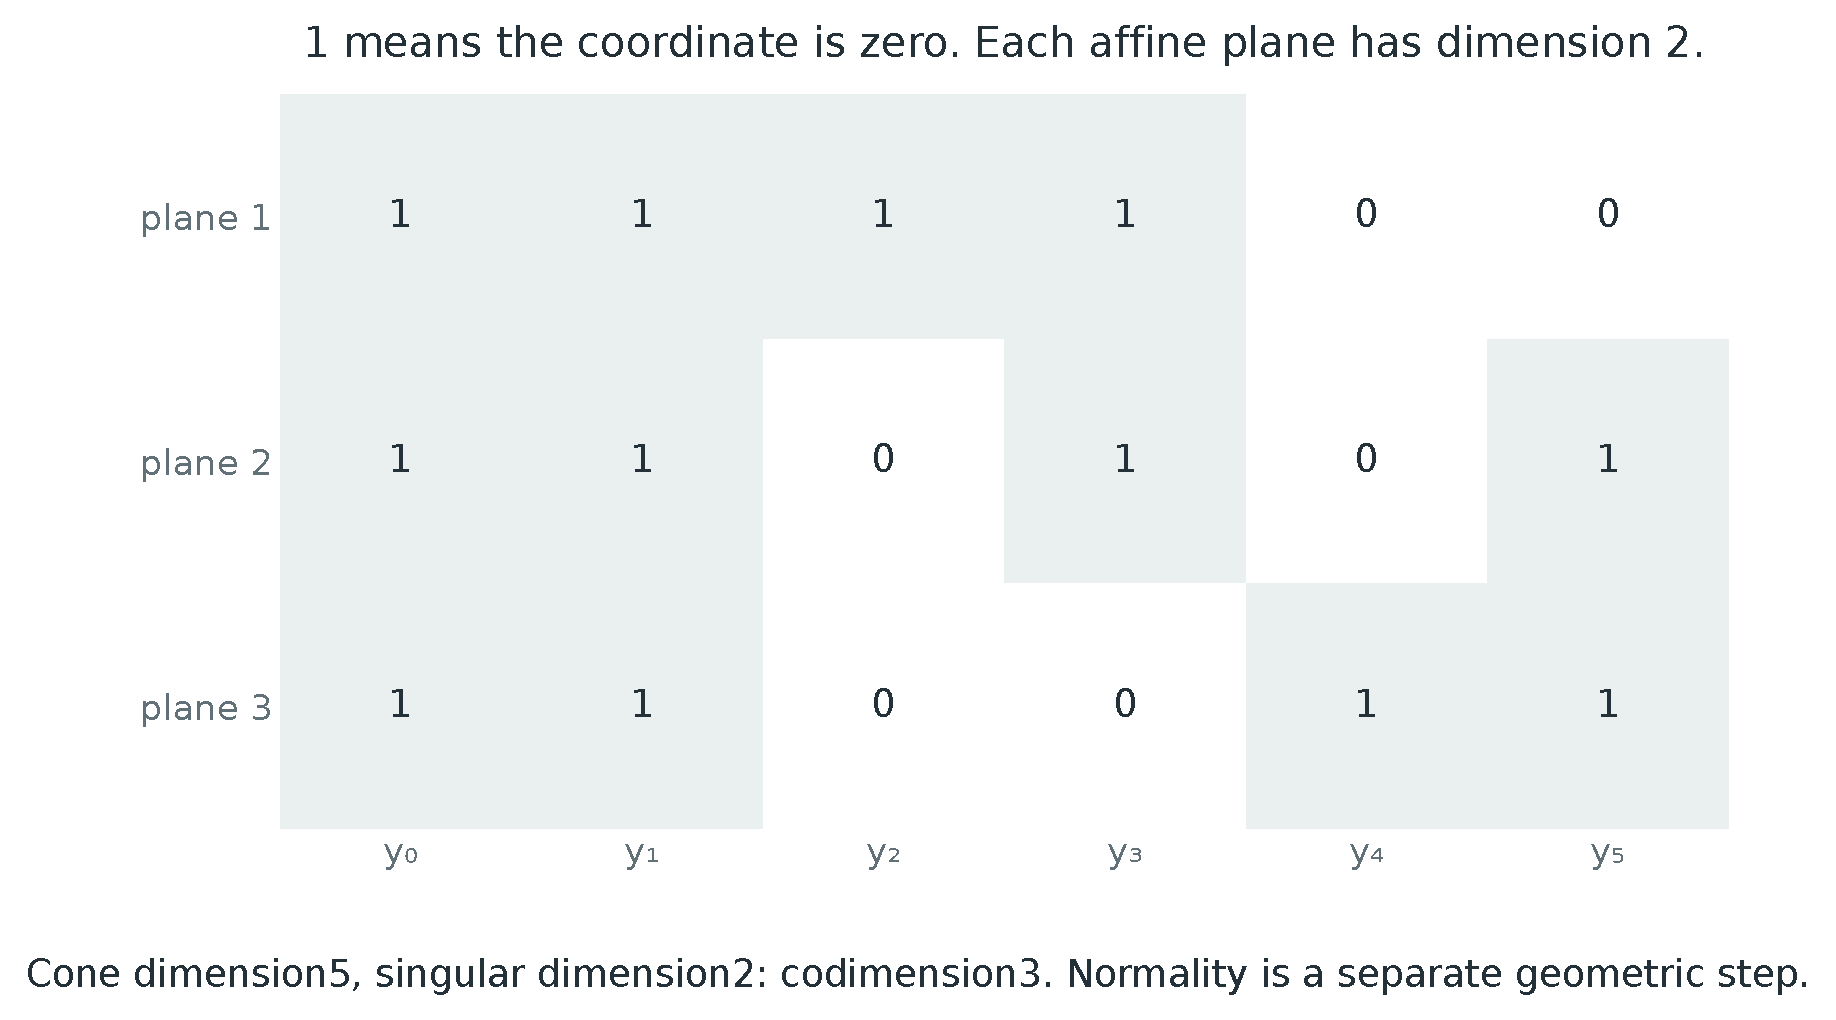
\includegraphics[width=0.98\linewidth]{21_carrier70_singular_locus.pdf}\caption{The certified coordinate singular planes. Normality uses their codimension in the cone.}\end{figure}

\hypertarget{carrier70-why-a-resolution-is-uniruled}{%
\section{Why a resolution is
uniruled}\label{carrier70-why-a-resolution-is-uniruled}}

Take a projective resolution \(r:\widetilde Y\to Y\) which is an
isomorphism over \(U_Y\). A general complete-intersection curve \(C\)
cut out by three sufficiently ample Cartier divisors avoids the singular
locus of \(Y\), which has dimension at most two. Its strict transform
avoids the exceptional divisors. Therefore

\[
K_{\widetilde Y}\cdot\widetilde C=K_Y\cdot C=-3H\cdot C<0.
\]

These curves move in a covering family. Thus \(K_{\widetilde Y}\) is not
pseudoeffective. The theorem of Boucksom--Demailly--Păun--Peternell
implies that \(\widetilde Y\) is uniruled.

No assertion of log terminal singularities, rational connectedness, or
Fano positivity on the resolution is used.

The rational Hodge conjecture for smooth projective uniruled fourfolds
is a proved theorem of Conte--Murre, also stated as Corollary 4.2 of
Arapura, arXiv:0706.2506. Therefore every rational \((2,2)\)-class on
\(\widetilde Y\) is algebraic.

For context, this theorem does not use the unknown general fourfold
case: a uniruled fourfold is dominated generically finitely by a
resolution of \(T\times\mathbf P^1\), with \(\dim T=3\). The relevant
Hodge classes on the product are algebraic by the threefold case and
Künneth, blowup centers have dimension at most two, push-pull transfers
algebraicity.

\hypertarget{carrier70-the-packet-is-actually-carried-by-this-cover}{%
\section{The packet is actually carried by this
cover}\label{carrier70-the-packet-is-actually-carried-by-this-cover}}

It remains to verify that the target is not merely a convenient variety
unrelated to the desired character.

Direct computation gives

\[
A^Ta=70\beta,\qquad \beta=(3,3,1,3,2,3),
\]

and hence \(B^T\beta=\alpha\). To obtain a genuine character of the
projective torus, let \(r_0=(0,0,2,0,0,3)\) be the first row of \(A\)
and set

\[
u=\beta-3r_0=(3,3,-5,3,2,-6).
\]

Then

\[
W\cdot u=0,\qquad B^Tu=\alpha-630e_0.
\]

Thus \(u\) is a character of the weighted projective torus. Its pullback
restricts on \(G_{210}\) to the Fermat character \(\alpha\), since
\(630=3\cdot210\).

Let \(K\) be the kernel of the torus isogeny. The relation \(AB=210I\)
shows that \(K\) embeds in \(G_{210}\): an element in the kernel has
representatives whose 210th powers are all the same, and a common scalar
makes them roots of unity. The displayed character identity proves
\(\chi_\alpha|_K=1\). The same holds for every rational conjugate.
Therefore the whole rational packet is \(K\)-invariant.

\hypertarget{carrier70-boundary-control-and-hodge-lifting}{%
\section{Boundary control and Hodge
lifting}\label{carrier70-boundary-control-and-hodge-lifting}}

\hypertarget{carrier70-no-full-support-packet-is-lost-at-the-fermat-boundary}{%
\subsection{No full-support packet is lost at the Fermat
boundary}\label{carrier70-no-full-support-packet-is-lost-at-the-fermat-boundary}}

The coordinate boundary of \(X_{210}\) is a simple normal crossing
divisor. Every nonempty coordinate stratum is fixed pointwise by at
least one coordinate scaling subgroup \(\mu_{210}\). Our full-support
character is nontrivial on that subgroup. The same is true for every
character in its rational orbit.

In the boundary Gysin spectral sequence, the corresponding character
projector therefore kills every boundary term. The normal
orientation/Tate factors have trivial coordinate-scaling action.
Consequently restriction induces an isomorphism on the packet:

\[
e_{[\alpha]}H^4(X_{210},\mathbf Q)
\xrightarrow{\sim}
e_{[\alpha]}H^4(U_{210},\mathbf Q).
\]

This argument is independent of any asserted torus-residue extension for
singular weighted hypersurfaces.

\hypertarget{carrier70-descent-to-the-open-carrier}{%
\subsection{Descent to the open
carrier}\label{carrier70-descent-to-the-open-carrier}}

Because \(q\) is finite étale with deck group \(K\),

\[
q^*:H^4(U_Y,\mathbf Q)
\xrightarrow{\sim}H^4(U_{210},\mathbf Q)^K.
\]

This is an isomorphism of mixed Hodge structures onto its image.
Normalized transfer supplies the inverse. The rational pure
\((2,2)\)-packet therefore descends to a pure weight-four Hodge
substructure of \(H^4(U_Y,\mathbf Q)\).

\hypertarget{carrier70-lifting-is-justified-by-the-lowest-weight-theorem}{%
\subsection{Lifting is justified by the lowest-weight
theorem}\label{carrier70-lifting-is-justified-by-the-lowest-weight-theorem}}

Deligne's Corollary 3.2.17 in \emph{Théorie de Hodge II} gives

\[
W_4H^4(U_Y,\mathbf Q)
=\operatorname{im}\bigl(H^4(\widetilde Y,\mathbf Q)
\to H^4(U_Y,\mathbf Q)\bigr).
\]

Here \(W_4\) denotes the weight filtration, not the Fermat packet
notation. The descended classes have weight four, so belong to this
image. The category of polarizable pure rational Hodge structures is
semisimple. The surjection from \(H^4(\widetilde Y)\) onto its image
thus has a Hodge-theoretic section. Every descended rational
\((2,2)\)-class has a rational \((2,2)\)-lift on \(\widetilde Y\).

This lifting is not being inferred from an arbitrary complex residue
numerator. Rationality, purity, and the surjection of pure Hodge
structures have all been checked separately.

\hypertarget{carrier70-producing-the-algebraic-classes-and-returning-to-degree-70}{%
\section{Producing the algebraic classes and returning to degree
70}\label{carrier70-producing-the-algebraic-classes-and-returning-to-degree-70}}

By the uniruled-fourfold theorem, each lifted class on \(\widetilde Y\)
is a rational combination of algebraic surface classes. The resolved
graph of the monomial rational map

\[
X_{210}\dashrightarrow\widetilde Y
\]

defines an algebraic correspondence. Its pullback on cohomology agrees
with \(q^*\) on the torus. Apply the rational orbit projector
\(e_{[\alpha]}\), which is a rational linear combination of graphs of
diagonal automorphisms. Therefore it preserves the span of algebraic
cycle classes.

The resulting class and the prescribed class agree on \(U_{210}\), their
difference lies in the packet and restricts to zero. The preceding
boundary isomorphism proves that difference is zero. This establishes
algebraicity of the entire \(W_{[\alpha]}\) packet on \(X_{210}\).

Finally, use the finite coordinate-cube map

\[
\pi:X_{210}\longrightarrow X_{70},\qquad
[x_i]\longmapsto[x_i^3].
\]

Its pullback identifies \(W_{[a]}\) with \(W_{[3a]}\). The identity

\[
\pi_*\pi^*=(\deg\pi)\operatorname{id}
\]

then transports the algebraic classes down to \(X_{70}\). Division by
the positive degree is legitimate because all cycle coefficients are
rational.

For arbitrary \(k\ge1\), the coordinate-power map \(X_{70k}\to X_{70}\)
pulls the same packet back algebraically. This proves the stated
infinite family of packets. It does not prove the full Hodge conjecture
for those varieties.

\hypertarget{carrier70-reusable-criterion-and-the-remaining-universal-problem}{%
\section{Reusable criterion and the remaining universal
problem}\label{carrier70-reusable-criterion-and-the-remaining-universal-problem}}

The argument proves this criterion:

\textbf{Torus-carrier criterion.} Let \(W\) be a full-support rational
middle Hodge packet on a Fermat fourfold. Suppose a finite torus isogeny
identifies its open Fermat variety with the inverse image of a smooth
torus hypersurface, the deck group acts trivially on \(W\), and that
torus hypersurface has a smooth projective compactification for which
the rational degree-four Hodge conjecture is known. Then \(W\) is
algebraic.

A normal, well-formed weighted hypersurface with negative canonical
hyperplane coefficient supplies one such compactification after
resolution: the resolution is uniruled by the uniruledness argument
above.

For searching, choose nonnegative integral columns \(v_j\) satisfying
\(a\cdot v_j\equiv0\pmod m\). Seek a nonsingular six-column matrix \(A\)
with

\[
A^{-1}\mathbf1>0,\qquad \mathbf1^TA^{-1}\mathbf1>1.
\]

These inequalities discover candidate weights only. Normality and
codimension of the ambient singular intersections still require
geometric certificates.

\textbf{Matrix-carrier corollary.} Let \(a\) be a full-support balanced
rational Hodge character modulo \(m\). Suppose \(A\) is a nonsingular
nonnegative integral \(6\times6\) matrix such that

\[
A^Ta\in m\mathbf Z^6,\qquad A^{-1}\mathbf1>0,
\qquad\mathbf1^TA^{-1}\mathbf1>1.
\]

Let \(W/D=A^{-1}\mathbf1\), with primitive positive integral weights
\(W\), and assume the row-monomial hypersurface is integral, normal, and
well formed in \(\mathbf P(W)\). Then the rational Fermat packet
\(W_{[a]}\) is algebraic.

Indeed, choose \(M\) divisible by \(m\) and all denominators of
\(A^{-1}\). Put \(B=MA^{-1}\), \(\alpha=(M/m)a\), and \(\beta=A^Ta/m\).
For any row \(r_i\) of \(A\),

\[
u=\beta-3r_i,\qquad W\cdot u=0,\qquad
B^Tu=\alpha-3Me_i.
\]

Here \(W\cdot\beta=3D\) follows from \(\sum a_j=3m\). Thus deck
invariance follows uniformly from the matrix congruence, it is not an
extra conjecture. The positive weight sum gives negative canonical
coefficient, normality and well-formedness justify the canonical
computation, and the uniruledness, descent, lifting and return arguments
above finish the proof. This corollary replaces an assumed cycle seed
with a finite exponent matrix and checkable geometric hypotheses.

There is no proof here that such carriers exist for every balanced
packet. Still less is there a reduction of arbitrary smooth projective
varieties to these diagonal Fermat packets. Those are the missing
universal coverage statements, they are not consequences of the
successful example.

The earlier proposed fixed-degree central-defect realization lemma
remains unproved and is not used anywhere in this proof. Likewise, this
construction does not establish the general CM half-twist Chow
correspondence listed as open in the pre-existing Komorebi manuscript.

\hypertarget{carrier70-computation-audit}{%
\section{Computation audit}\label{carrier70-computation-audit}}

The narrower atomic chain/loop search considered 6,600 labeled graphs
and 24 unit conjugates, for 158,400 pairs. Its maximum normalized weight
sum was \(296/315<1\), it found no Fano candidate in that implemented
family. A broader functional-graph search also failed to find one. These
failures are not evidence against the Hodge conjecture.

The unrestricted column search enumerated 1,955 invariant columns of
total degree at most 18. A floating-point linear program selected a
six-column support. Its result was then replaced by exact rational
matrix arithmetic. The actual certificate and all conclusions about the
selected matrix are independent of floating-point tolerances.

The final verifier checks 24 assertions, including every unit conjugate,
matrix identities, all ambient coordinate singular strata, and the exact
radical-gradient ideal certificate. It does not compute algebraic
cycles, formally prove mixed Hodge theory, or independently authenticate
the cited geometric theorems.

\hypertarget{transfer210-carrier-transfer-and-obstructions-for-fermat-hodge-packets}{%
\chapter{Carrier transfer and obstructions for Fermat Hodge
packets}\label{transfer210-carrier-transfer-and-obstructions-for-fermat-hodge-packets}}

\textbf{Komorebi P. --- research block v0.2.0}\\
\textbf{Status:} manuscript-level mathematical arguments with exact
computational certificates. The geometric argument is not formally
verified or peer reviewed. Exact certificates were independently
replayed for this edition. The degree-210 algebraicity conclusion uses
the degree-70 carrier proposition from v0.1.0 and explicitly identified
classical results. No general Hodge-conjecture solution or historical
novelty claim is made.

\hypertarget{transfer210-main-results-and-proof-boundaries}{%
\section{Main results and proof
boundaries}\label{transfer210-main-results-and-proof-boundaries}}

Let

\[
X_m^n=\{x_0^m+\cdots+x_{n+1}^m=0\}\subset\mathbf P^{n+1}_{\mathbf C}.
\]

This block obtains three different kinds of results.

\begin{enumerate}
\def\labelenumi{\arabic{enumi}.}
\tightlist
\item
  \textbf{Algebraicity transfer.} The rational primitive Hodge packet
  associated to \[
  b=(2,9,129,142,168,180)\pmod {210}
  \] is algebraic, using the v0.1.0 degree-70 carrier proposition and
  classical Fermat cycle correspondences. Its rational dimension is 48.
  Its full conductor is 210, so it is not a coordinate-power inflation
  of a lower-conductor packet. A 14-term signed identity supplies the
  transfer.
\item
  \textbf{Global matrix obstruction.} No nonnegative integral matrix
  capturing this packet can have positive normalized weights whose sum
  exceeds one. This is proved for every matrix size-six candidate of the
  previous criterion, not just for a bounded search. An exact dual
  certificate has two independent finite verifications, with a uniform
  argument covering all larger columns.
\item
  \textbf{Structural obstructions.} An infinite balanced family also
  cannot have such a matrix. A separate holomorphic-character-power
  criterion excludes all direct diagonal-quotient uniruled carriers for
  six explicitly checked test packets.
\end{enumerate}

The positive transfer and negative matrix result are compatible. They
prove that the direct matrix method is incomplete even on packets that
can be made algebraic by combining a geometric seed with classical cycle
operations.

The new standalone verifier checks 46 finite assertions. The preserved
predecessor verifier was separately rerun and passed all 24 of its
checks. Neither count is a formal verification of the geometric
theorems.

\hypertarget{transfer210-character-conventions}{%
\section{Character conventions}\label{transfer210-character-conventions}}

A full-support character is an ordered tuple \(a=(a_0,\ldots,a_{n+1})\)
of nonzero residues modulo \(m\), with sum zero modulo \(m\). Its
eigenspace in primitive cohomology is a complex line. For even \(n\),
its rational Galois packet is of middle Hodge type precisely when

\begin{equation}\label{eq:transfer210-2.1}
\sum_i\langle ta_i\rangle_m=\frac{n+2}{2}m
\quad\text{for every }t\in(\mathbf Z/m\mathbf Z)^\times.\end{equation}

Here residues are least positive representatives. This is the classical
Fermat character decomposition, see \cite{DaSilvaFermat}, Theorem 2.1.
Rational orbit dimension means the number of distinct \textbf{ordered}
unit conjugates, not the number of representatives after coordinate
permutations.

Write \(\nu(a)\) for its integer residue-multiplicity vector. Write
\(a\uplus b\) for concatenation regarded as a multiset. Permuting
coordinates is an algebraic automorphism, so multiset identities suffice
for algebraicity transfer. Write \(-a\) for coordinatewise negation
modulo \(m\).

A character is called algebraic when its eigenspace is contained in the
complex span of algebraic cycle classes. The rational orbit then lies in
the rational algebraic-cycle subspace: this subspace and the orbit
projector are rational, and the projector is a rational linear
combination of graphs of diagonal automorphisms.

\hypertarget{transfer210-classical-inputs-stated-separately-from-computation}{%
\section{Classical inputs, stated separately from
computation}\label{transfer210-classical-inputs-stated-separately-from-computation}}

We use the following established operations.

\textbf{Concatenation.} Algebraic balanced characters concatenate to an
algebraic character on the higher-dimensional Fermat variety.

\textbf{Complementary-pair removal.} If a character becomes algebraic
after concatenating any finite collection of pairs \((r,m-r)\), then it
was algebraic already.

These are the Shioda--Ran results recorded as Aoki \cite{Aoki}, Theorem
1-4(i),(ii). The equivariant Fermat join construction is also described
in \cite{DaSilvaFermat}, Theorem 2.2 and Corollary 2.3. The removal
operation is a geometric correspondence theorem, not a formal assumption
that arbitrary tensor factors can be cancelled.

\textbf{Four-entry blocks.} Every rational balanced four-entry packet is
algebraic, by the Lefschetz (1,1) theorem for the corresponding Fermat
surface.

\textbf{Standard blocks.} For an odd prime \(p\mid m\), put \(d=m/p\).
Aoki \cite{Aoki}, Theorem 2-1 constructs an algebraic cycle representing

\[
\sigma_{p,i}=(i,i+d,\ldots,i+(p-1)d,m-pi)
\]

under the relevant nonzero-entry and coprimality conditions. We only use
\((m,p,i)=(35,5,5)\) and \((35,7,2)\). Here \(\gcd(5,7)=\gcd(2,5)=1\),
and all entries are nonzero.

\textbf{Power transport.} The finite coordinate-power morphism
\(X_{km}^n\to X_m^n\) transports algebraic cycle classes by pullback.
The character is multiplied by \(k\).

\hypertarget{transfer210-source-access-boundary}{%
\subsection{Source-access boundary}\label{transfer210-source-access-boundary}}

The October audit obtained the original Aoki article. Theorem 1-4 states
concatenation and removal of complementary-pair auxiliary blocks.
Theorem 2-1 supplies the standard blocks below under its actual
nonzero-entry and coprimality conditions. The September source-access
limitation is preserved in the evidence archive and resolved for these
specific leaves in this edition. Neither theorem allows cancellation of
an arbitrary motive. The Shioda--Ran original proofs were not
independently re-audited.

\hypertarget{transfer210-the-inherited-geometric-seed}{%
\section{The inherited geometric
seed}\label{transfer210-the-inherited-geometric-seed}}

The authoritative predecessor is the included, unchanged archive

\texttt{predecessor/Komorebi\_Hodge\_Carrier70\_v0.1.0.zip}.

Its proposition asserts algebraicity of the 24-dimensional rational
packet

\begin{equation}\label{eq:transfer210-4.1}
a=(1,20,24,42,61,62)\pmod {70}.\end{equation}

The proof uses a concrete monomial correspondence to a normal weighted
degree-30 hypersurface with weights \((10,6,3,3,3,8)\). Its resolution
is shown to be uniruled, so the Conte--Murre Hodge theorem for uniruled
fourfolds applies. See \cite{ArapuraUniruled}, Corollary 4.2. Boundary
vanishing, finite étale descent and lowest-weight lifting then transfer
cycles back.

The predecessor's singular-locus, matrix and character checks have been
replayed, see \texttt{results/predecessor\_verification.json}. This does
not replace review of the predecessor's mixed-Hodge and birational
arguments.

Pullback under \(X_{210}^4\to X_{70}^4\) gives the algebraic source
packet

\begin{equation}\label{eq:transfer210-4.2}
s=3a=(3,60,72,126,183,186)\pmod {210}.\end{equation}

The source has conductor 70 and 24 distinct ordered unit conjugates. The
new target

\begin{equation}\label{eq:transfer210-4.3}
b=(2,9,129,142,168,180)\pmod {210}\end{equation}

has conductor 210 and 48 distinct ordered unit conjugates. Every
conjugate of both tuples sums to 630. Their Galois orbits are disjoint.
These are exact finite checks.

The target also occurs in the even-degree residual table accompanying
\cite{Jumagulov2026}. We use that table to select a research target, not
as proof that the entire census is correct or that this exact packet was
previously unknown in all literature.

\begin{figure}[tbp]\centering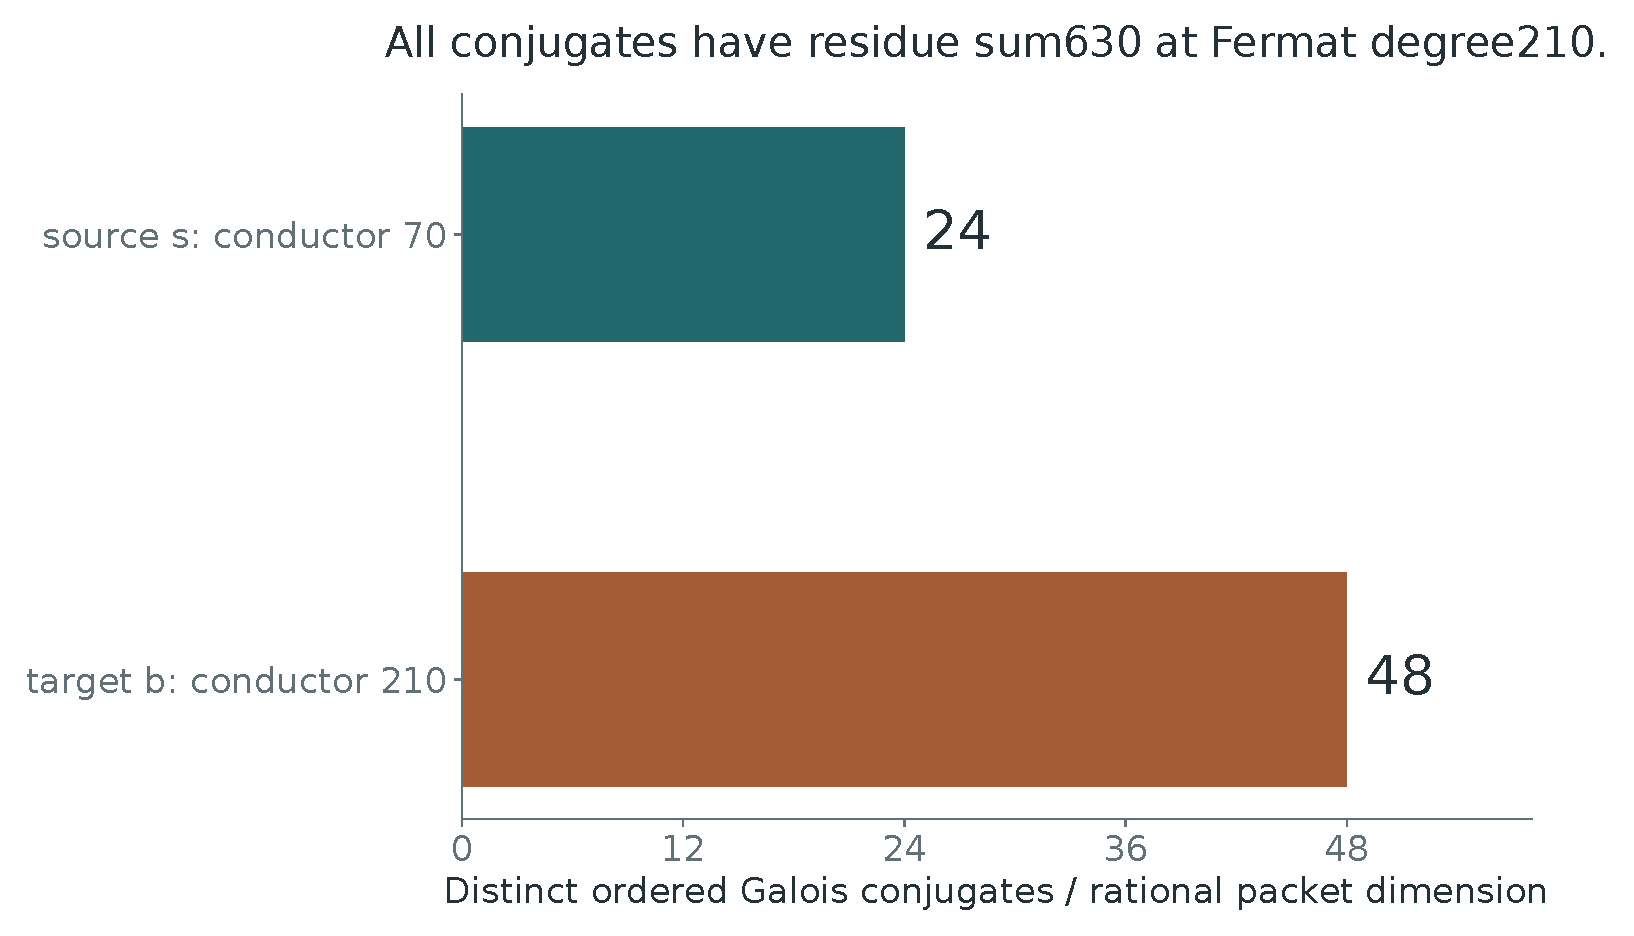
\includegraphics[width=0.98\linewidth]{23_transfer210_orbits.pdf}\caption{Source and target ordered unit orbits have dimensions 24 and 48, with conductors 70 and 210.}\end{figure}

\hypertarget{transfer210-an-exact-transfer-identity}{%
\section{An exact transfer identity}\label{transfer210-an-exact-transfer-identity}}

All entries in this section are modulo 210. Define

\[
P_k=(k,210-k)
\]

and

\[
\begin{aligned}
Q_3&=(3,105,108,204),\\
Q_9&=(9,105,114,192),\\
Q_{24}&=(24,105,129,162),\\
Q_{27}&=(27,105,132,156),\\
R_2&=(2,72,142,204).
\end{aligned}
\]

Every one of these four-entry blocks is balanced, as the exact verifier
checks against every unit modulo 210. They are algebraic by the surface
case.

Define the two longer blocks

\[
S_5=(30,60,72,114,156,198),
\qquad
S_7=(12,42,72,102,126,132,162,192).
\]

Their deflations are

\[
\begin{aligned}
S_5/6&=(5,10,12,19,26,33)=\sigma_{5,5}\quad\text{at degree }35,\\
S_7/6&=(2,7,12,17,21,22,27,32)=\sigma_{7,2}\quad\text{at degree }35,
\end{aligned}
\]

up to ordering. The standard-cycle theorem and power pullback make both
blocks algebraic. The length-eight block lives on a Fermat sixfold, only
its explicitly known standard cycle is needed, not the general Hodge
conjecture for that sixfold.

The exact identity is

\begin{equation}\label{eq:transfer210-5.1}
\boxed{
\begin{aligned}
 b\uplus P_{24}\uplus P_{27}\uplus P_{105}\uplus Q_3\uplus S_5\uplus S_7
 ={}&s\uplus P_{12}\uplus P_{30}\uplus P_{42}\uplus P_{102}\\
 &\uplus Q_9\uplus Q_{24}\uplus Q_{27}\uplus R_2.
\end{aligned}}\end{equation}

Both sides contain exactly 30 entries, with equal multiplicity of every
residue. Equivalently, \(\nu(b)-\nu(s)\) is the signed sum of the
fourteen displayed auxiliary generators, each with coefficient \(+1\) or
\(-1\). The certificate is stored in \texttt{results/transfer210.json}.

\hypertarget{transfer210-algebraicity-of-the-degree-210-packet}{%
\subsection{Algebraicity of the degree-210
packet}\label{transfer210-algebraicity-of-the-degree-210-packet}}

Assuming the inherited degree-70 carrier proposition, every rational
class in \(W_{[b]}\) is algebraic.

\textbf{Proof.} Let \(L\) be the auxiliary multiset to the left of \eqref{eq:transfer210-5.1}
and \(R\) the auxiliary multiset to its right. Thus

\[
b\uplus L=s\uplus R,
\qquad |L|=|R|=24.
\]

All component packets of \(L\) and \(R\) are algebraic. Negation
preserves their algebraicity, either by the rational Galois packet
statement or by conjugating the corresponding cycle class. Append \(-L\)
to both sides:

\begin{equation}\label{eq:transfer210-5.2}
b\uplus L\uplus(-L)=s\uplus R\uplus(-L).\end{equation}

The right-hand side is algebraic by concatenation, because the source
and every auxiliary component are algebraic. The left-hand auxiliary
part \(L\uplus(-L)\) is a multiset of exactly 24 complementary pairs.
The full character has 54 entries and is a character on
\(X_{210}^{52}\). Complementary-pair removal therefore gives
algebraicity of \(b\) on \(X_{210}^4\).

The character projector and its rational Galois orbit transfer this
statement to every class in \(W_{[b]}\). Its dimension is 48. This
proves the proposition. \hfill\ensuremath{\square}

For every \(k\ge1\), coordinate-power pullback gives the associated
packet on \(X_{210k}^4\). It does not establish the Hodge conjecture for
all packets on any of these fourfolds.

This proof does not subtract unknown algebraic cycles, assert
cancellation of arbitrary motives, or assume a cycle-existence theorem
for the new packet. Every negative coefficient in the incidence identity
is removed through explicitly algebraic auxiliary blocks and the
classical complementary-pair theorem.

\begin{figure}[tbp]\centering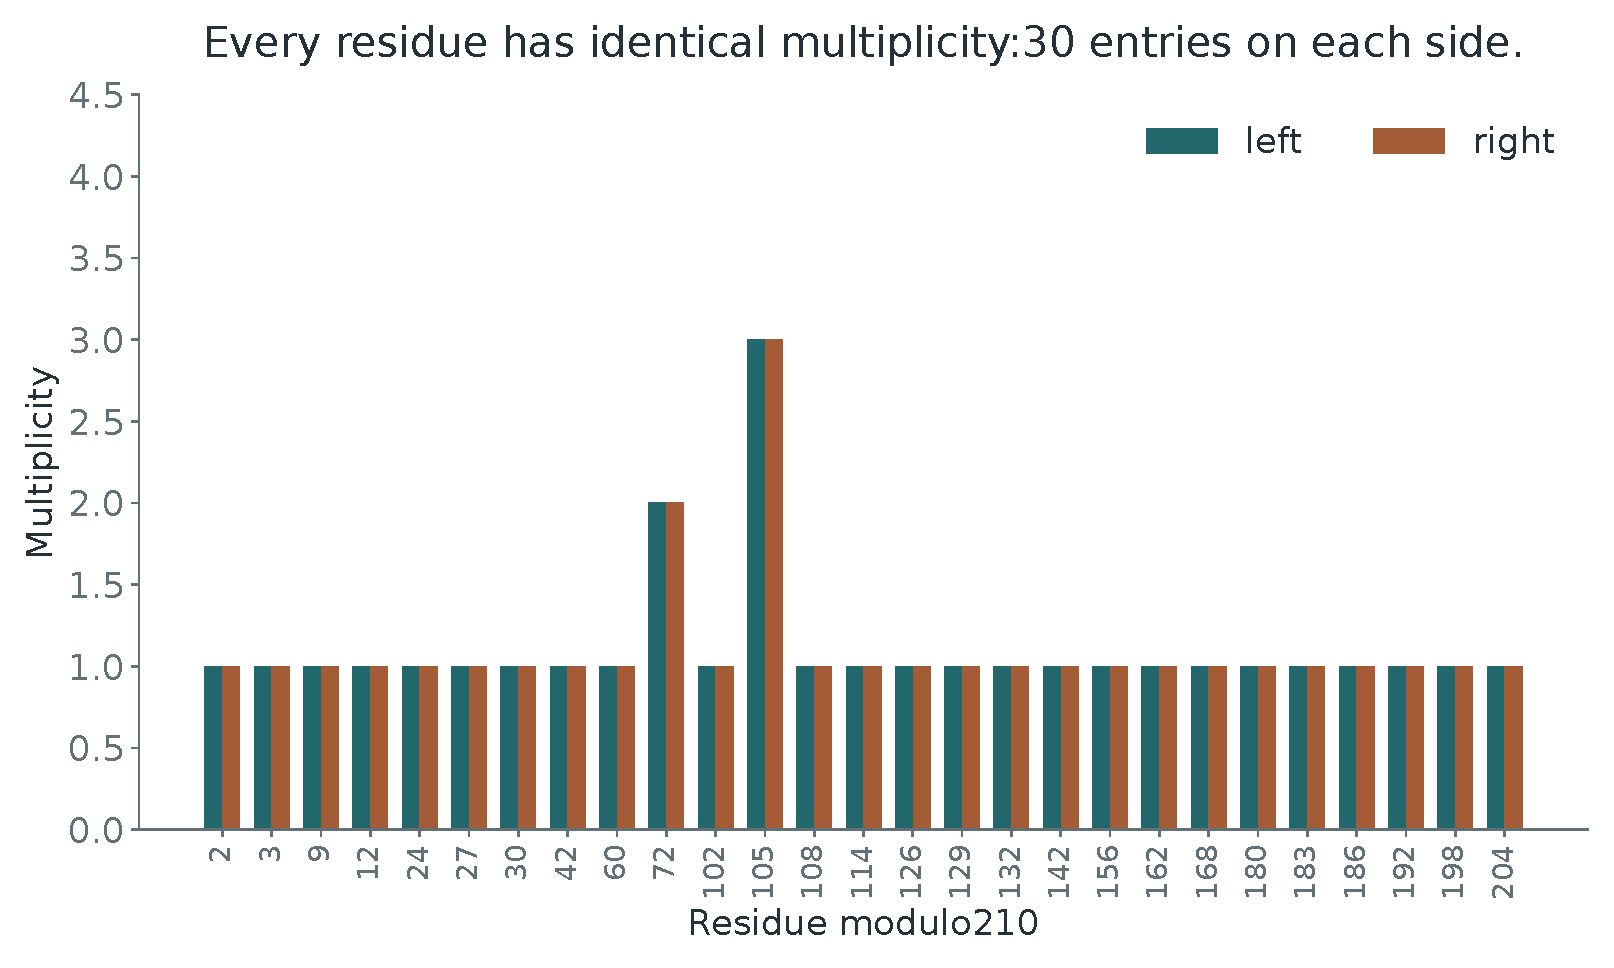
\includegraphics[width=0.98\linewidth]{24_transfer210_incidence.pdf}\caption{An exact signed multiplicity equality. Its algebraic implication also uses the stated classical correspondence operations.}\end{figure}

\hypertarget{transfer210-a-global-obstruction-to-the-direct-matrix-route}{%
\section{A global obstruction to the direct matrix
route}\label{transfer210-a-global-obstruction-to-the-direct-matrix-route}}

The previous search criterion required a nonsingular nonnegative
integral matrix \(A\), with columns \(v_j\), satisfying

\begin{equation}\label{eq:transfer210-6.1}
b\cdot v_j\equiv0\pmod {210},\qquad
w=A^{-1}\mathbf1>0,\qquad
\sum_jw_j>1.\end{equation}

The following exact certificate rules this out for the new target.

Set

\begin{equation}\label{eq:transfer210-6.2}
\eta=\frac1{420}(31,87,57,101,84,60).\end{equation}

Its coordinates are positive and sum to one. For every nonzero
\(v\in\mathbf Z_{\ge0}^6\) satisfying \(b\cdot v\equiv0\pmod {210}\),

\begin{equation}\label{eq:transfer210-6.3}
\boxed{\eta\cdot v\ge1.}\end{equation}

\hypertarget{transfer210-proof-of-the-universal-inequality}{%
\subsection{Proof of the universal
inequality}\label{transfer210-proof-of-the-universal-inequality}}

If \(|v|\ge14\), the numerator of \(\eta\cdot v\) is at least
\(14\cdot31=434>420\). It therefore suffices to check \(1\le |v|\le13\).

The exact verifier enumerates all 27,131 such nonnegative six-tuples.
Exactly 143 satisfy the invariant-column congruence. Each has numerator
at least 420, and the minimum is exactly 420. The enumerator uses
integer arithmetic only and includes all compositions in the specified
range. Together with the large-degree bound, this proves \eqref{eq:transfer210-6.3} for every
column, not just those within a search cutoff.

As an independent implementation, place residue states in
\(\mathbf Z/210\) and give the six transitions \(r\mapsto r+b_i\)
integer costs \((31,87,57,101,84,60)\). A nonempty zero-sum column is a
return walk. Exact shortest-path computation finds minimum nonempty
return cost 420. All costs are positive. This verifies the same
inequality by a different method.

\hypertarget{transfer210-no-direct-positive-weight-matrix-carrier}{%
\subsection{No direct positive-weight matrix
carrier}\label{transfer210-no-direct-positive-weight-matrix-carrier}}

If a matrix in \eqref{eq:transfer210-6.1} existed, then

\[
1=\eta^T\mathbf1=\eta^TAw
 =\sum_jw_j(\eta\cdot v_j)\ge\sum_jw_j.
\]

This contradicts \(\sum_jw_j>1\). \hfill\ensuremath{\square}

The single invariant column \(v=\mathbf1\), with coefficient one,
supplies a matching value-one witness for the relaxed column linear
program. Thus its global optimum is exactly one. This is not a claim
that a nonsingular six-column positive solution attains that optimum.

The invariant-column condition is unchanged by unit-conjugating \(b\),
permuting its coordinates with the corresponding dual permutation, or
inflating \(b\) and the modulus together. The obstruction persists under
those operations.

the algebraicity-transfer proposition above and the direct-matrix
obstruction corollary above together show a definite limitation of the
direct carrier criterion: a packet can be algebraic by a certified
transfer while every direct matrix of this type is excluded. This does
not rule out all geometric carriers or non-diagonal correspondences.

\begin{figure}[tbp]\centering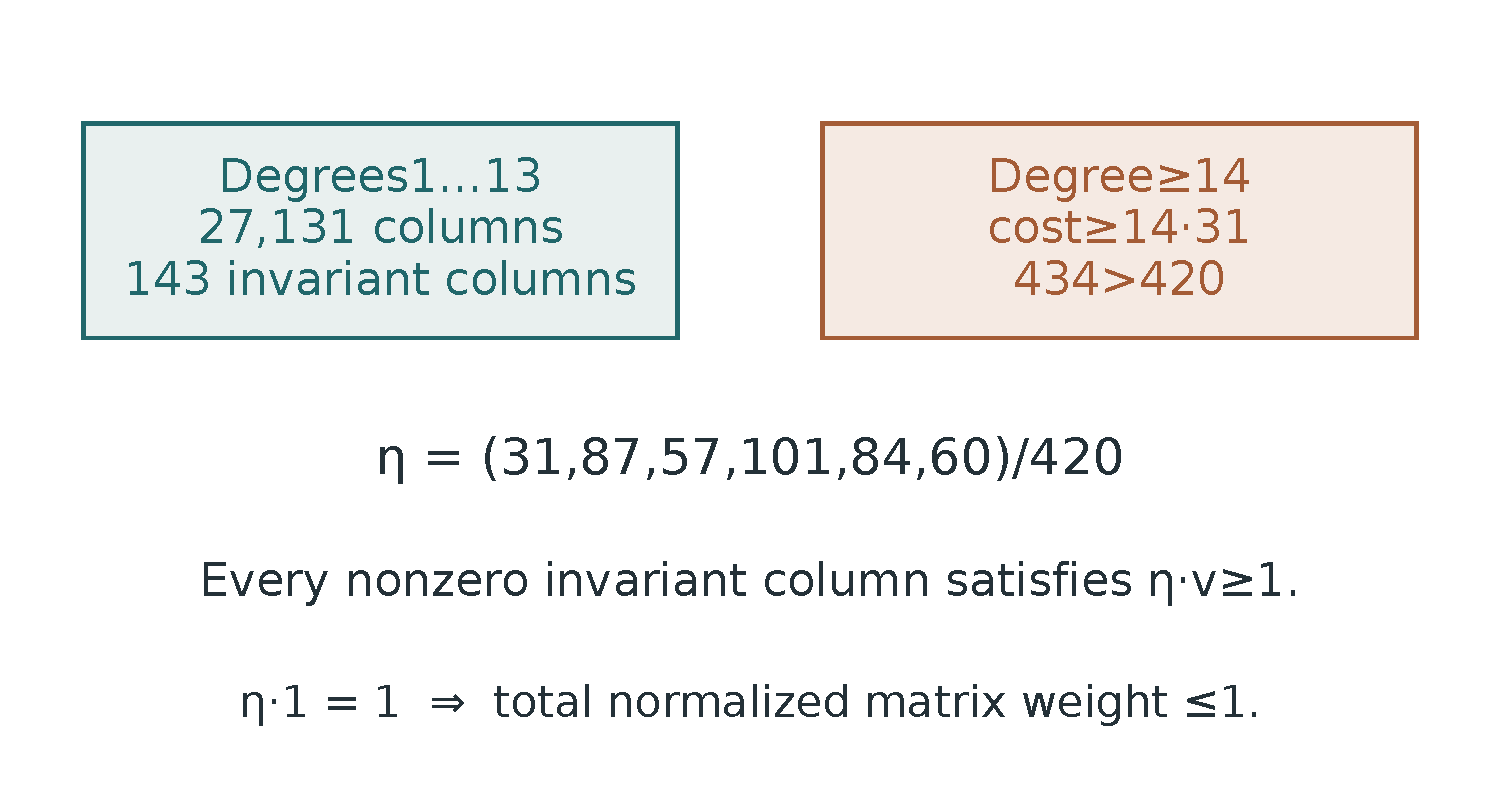
\includegraphics[width=0.98\linewidth]{27_global_dual210.pdf}\caption{The exact global dual combines a complete finite premise with a uniform large-degree inequality.}\end{figure}

\hypertarget{transfer210-a-uniform-infinite-family-excluded-by-the-same-criterion}{%
\section{A uniform infinite family excluded by the same
criterion}\label{transfer210-a-uniform-infinite-family-excluded-by-the-same-criterion}}

For any integer \(q>5\), let

\begin{equation}\label{eq:transfer210-7.1}
a_q=(1,1+q,1+2q,1+3q,1+4q,5q-5)\pmod {5q}.\end{equation}

\hypertarget{transfer210-theorem-7.2}{%
\subsection{Theorem 7.2}\label{transfer210-theorem-7.2}}

Every \(a_q\) is a full-support middle-balanced character. No matrix
satisfying the previous direct positive-weight criterion exists for
\(a_q\).

\textbf{Proof of balance.} Let \(t\) be a unit modulo \(5q\), and let
\(s\) be its least positive residue modulo \(q\). The first five
multiplied residues permute

\[
s,s+q,s+2q,s+3q,s+4q.
\]

Their sum is \(5s+10q\). The last multiplied residue is \(5(q-s)\), so
the total is \(15q=3(5q)\).

\textbf{Proof of the obstruction.} Set

\[
\eta_q=\frac1q(1,1,1,1,1,q-5).
\]

This vector is positive and has sum one. For a nonzero invariant column
\(v\ge0\), put \(S=v_0+\cdots+v_4\). Reducing
\(a_q\cdot v\equiv0\pmod {5q}\) modulo \(q\) gives
\(S-5v_5\equiv0\pmod q\). Therefore

\[
\eta_q\cdot v=\frac{S+(q-5)v_5}{q}
=\frac{S-5v_5}{q}+v_5
\]

is a positive integer, and hence at least one. Apply the same matrix
inequality as in the preceding dual argument. \hfill\ensuremath{\square}

This is a proof for every \(q>5\), not an extrapolation from finite
runs. The verifier's checks for \(6\le q\le80\) are benchmarks only.
These packets are themselves the standard family \(\sigma_{5,1}\), so
the obstruction is to the method, not to algebraicity.

\hypertarget{transfer210-a-stronger-obstruction-holomorphic-powers-of-a-hodge-character}{%
\section{A stronger obstruction: holomorphic powers of a Hodge
character}\label{transfer210-a-stronger-obstruction-holomorphic-powers-of-a-hodge-character}}

\hypertarget{transfer210-proposition-8.1}{%
\subsection{Proposition 8.1}\label{transfer210-proposition-8.1}}

Let \(a\) be a full-support Fermat fourfold character. Suppose some
integer multiple

\[
c=ka\pmod m
\]

has all entries nonzero and least-positive residue sum \(m\). A direct
quotient by a subgroup of the diagonal automorphism group that captures
\(a\) cannot have a smooth projective uniruled compactification.

\textbf{Proof.} If \(K\) is a diagonal deck subgroup and
\(\chi_a|_K=1\), then

\[
\chi_c|_K=\chi_a^k|_K=1.
\]

The residue description places the \(c\)-line in \(H^{4,0}\) under the
direct-action convention (or its conjugate under the inverse-character
convention). Its rational Galois span contains a nonzero \((4,0)\) part
and is also \(K\)-invariant.

Full support makes restriction to the open coordinate torus injective on
this character space. As in the predecessor, each boundary stratum is
fixed by a coordinate scaling subgroup on which the character is
nontrivial, so the relevant Gysin terms vanish. Finite étale descent
gives the invariant pure weight-four space on the open quotient.

For any smooth projective compactification, the lowest-weight image
theorem and the semisimplicity of polarizable pure Hodge structures lift
this space from open cohomology to compact cohomology. In particular the
compactification has a nonzero \(H^{4,0}\). These are the same classical
mixed-Hodge inputs as in the predecessor, see \cite{ArapuraUniruled},
\cite{DeligneHodgeII}.

A smooth projective uniruled fourfold has no nonzero holomorphic top
form: a generically finite dominant parametrization from a resolution of
a threefold times \(\mathbf P^1\) would pull such a form back
injectively, whereas the latter has none. This is a contradiction. \hfill\ensuremath{\square}

The assertion concerns this direct diagonal-quotient construction, not
arbitrary algebraic correspondences. It persists after coordinate-power
inflation of the source.

\Needspace{10\baselineskip}

\hypertarget{transfer210-exact-witnesses}{%
\subsection{Exact witnesses}\label{transfer210-exact-witnesses}}

{\small\begin{longtable}[]{@{}
  >{\raggedright\arraybackslash}p{(\columnwidth - 6\tabcolsep) * \real{0.2308}}
  >{\raggedright\arraybackslash}p{(\columnwidth - 6\tabcolsep) * \real{0.2308}}
  >{\raggedleft\arraybackslash}p{(\columnwidth - 6\tabcolsep) * \real{0.3077}}
  >{\raggedright\arraybackslash}p{(\columnwidth - 6\tabcolsep) * \real{0.2308}}@{}}
\toprule\noalign{}
\begin{minipage}[b]{\linewidth}\raggedright
Modulus
\end{minipage} & \begin{minipage}[b]{\linewidth}\raggedright
Middle-balanced character a
\end{minipage} & \begin{minipage}[b]{\linewidth}\raggedleft
k
\end{minipage} & \begin{minipage}[b]{\linewidth}\raggedright
Full-support character ka with sum m
\end{minipage} \\
\midrule\noalign{}
\endhead
\bottomrule\noalign{}
\endlastfoot
110 & (1,24,62,71,81,91) & 11 & (11,44,22,11,11,11) \\
110 & (1,31,55,71,81,91) & 11 & (11,11,55,11,11,11) \\
114 & (1,13,43,72,103,110) & 27 & (27,9,21,6,45,6) \\
114 & (1,13,43,80,102,103) & 9 & (9,3,45,36,6,15) \\
114 & (1,7,78,79,86,91) & 3 & (3,21,6,9,30,45) \\
220 & (1,62,111,142,162,182) & 11 & (11,22,121,22,22,22) \\
\end{longtable}}

Each source's middle balance and each product's nonzero entries and
residue sum are checked exactly. The multipliers are nonunits, so there
is no contradiction with the middle balance of all \textbf{unit}
conjugates of the source character.

These witnesses explain why merely increasing the direct diagonal
carrier search cannot address these targets. They do not show that the
targets are nonalgebraic.

\hypertarget{transfer210-computation-contract-failures-and-remaining-work}{%
\section{Computation contract, failures and remaining
work}\label{transfer210-computation-contract-failures-and-remaining-work}}

\hypertarget{transfer210-exact-final-replay}{%
\subsection{Exact final replay}\label{transfer210-exact-final-replay}}

\texttt{python\ checks/verify.py} needs Python 3.10 or later and only
its standard library. It runs without network access, optimization
software or floating-point arithmetic. It verifies the frozen identity,
all named character conditions, the standard-block deflations, the
54-entry stabilization, the dual's complete finite premise and degree
cutoff, an independent exact shortest-cycle check, six holomorphic-power
witnesses and 75 infinite-family benchmarks.

The code does not construct equations for a basis of representing
surfaces, verify the external theorems, or compile a proof in Lean. The
standard-block and carrier constructions give existence through known
algebraic correspondences, not a list of all representing surfaces.

\hypertarget{transfer210-discovery-distinct-from-proof}{%
\subsection{Discovery, distinct from
proof}\label{transfer210-discovery-distinct-from-proof}}

The transfer was found by a bounded mixed-integer search among
complementary pairs and standard blocks at degree 210. The solver uses
floating-point internals. The stored result has fourteen nonzero
coefficients and was accepted only after exact integer replay. Its
reported optimizer optimum is not a claim that fourteen is globally
minimal among all possible geometric identities.

An earlier Hermite-normal-form membership attempt exceeded its 20-second
execution allowance and was stopped without a conclusion. Direct
integer-programming discovery replaced it successfully. Bounded
degree-18 matrix scans were exploratory and never used as global
impossibility proofs. The exact dual arguments in the two dual
obstruction arguments above replace those bounded observations for the
targets they cover.

Original publisher PDF and some ancillary-log fetches failed. No missing
log was used as evidence, the transfer and its verification were
produced locally. The source-access limit for the classical Aoki theorem
is resolved in the source-access discussion above.

\hypertarget{transfer210-what-remains}{%
\subsection{What remains}\label{transfer210-what-remains}}

The general Hodge conjecture is not established. This block does not
cover all packets on \(X_{210}^4\), establish universal closure of the
Fermat packet calculus, or reduce arbitrary projective varieties to
diagonal hypersurfaces. It does not complete the earlier central-defect
realization lemma or a general CM half-twist Chow correspondence.

The direct matrix criterion cannot be the universal bridge: the two dual
obstruction arguments above disprove that assertion. Direct diagonal
uniruled quotients cannot capture the holomorphic-power examples either.
A further positive argument must therefore use stabilization and
transfer, a different known-algebraic carrier class, or genuinely
non-diagonal correspondences. That is a mathematical constraint on the
next construction, not a conjectured failure of Hodge.

\compactpart{Part XI. Global method obstructions and actual cycles}
\hypertarget{capacity_cycles-a-matrix-capacity-obstruction-and-explicit-five-phase-fermat-cycles}{%
\chapter{A matrix-capacity obstruction and explicit five-phase Fermat
cycles}\label{capacity_cycles-a-matrix-capacity-obstruction-and-explicit-five-phase-fermat-cycles}}

Komorebi research continuation, version 0.2.0. Session: 21 September
2026, America/Chicago.

\hypertarget{capacity_cycles-status-and-scope}{%
\section{Status and scope}\label{capacity_cycles-status-and-scope}}

This note contains manuscript proofs and replayable exact algebraic
certificates. It does not prove the general Hodge conjecture. The exact
certificates were independently replayed in October. The geometric
arguments are not formally verified or peer reviewed.

The positive algebraicity family reconstructed here is the \textbf{known
five-phase standard family of Aoki}. The October original-source audit
checked Theorem 2-1 of the 1987 paper. Its equations give the same
family after the Newton identities below. The construction is a direct
recomputation of those known surfaces. The determinant and period are
derived explicitly using the checked complete-intersection theorem of
Villaflor Loyola. No priority for the surfaces, equations, algebraicity
or determinant is claimed.

The concrete advances within this research attempt are:

\begin{enumerate}
\def\labelenumi{\arabic{enumi}.}
\tightlist
\item
  An exact global upper bound on the normalized weight sum of every
  invariant-column matrix candidate, with equality for the earlier
  degree-70 carrier.
\item
  A uniform obstruction showing that the earlier positive-anticanonical
  matrix criterion cannot cover all balanced Fermat packets, even with
  unbounded exponents and coordinate-power lifts.
\item
  Explicit complete-intersection surfaces, a uniform determinant
  identity, and nonzero exact periods for the infinite standard family
  missed by that criterion.
\end{enumerate}

The original v0.1.0 archive is preserved byte for byte in
\texttt{predecessor/}. Its original 24-check verifier was replayed
successfully before this continuation. The geometric arguments of the
predecessor have not been independently formally verified.

\hypertarget{capacity_cycles-conventions}{%
\section{Conventions}\label{capacity_cycles-conventions}}

Let

\[
X_m=\{F_m=x_0^m+\cdots+x_5^m=0\}\subset\mathbf P^5_{\mathbf C},
\qquad G_m=(\mu_m)^6/\mu_m.
\]

Write \(\langle r\rangle_m\) for the least-positive residue of a nonzero
residue class. A full-support character is

\[
a=(a_0,\ldots,a_5),\qquad 0<a_i<m,\qquad \sum a_i\equiv0\pmod m.
\]

The Griffiths residue basis of the Fermat hypersurface diagonalizes the
action of \(G_m\). The monomial \(x_0^{a_0-1}\cdots x_5^{a_5-1}\) at
pole order three gives the character of middle Hodge type when
\(\sum a_i=3m\). The entire rational orbit has type \((2,2)\) when

\begin{equation}\label{eq:capacity_cycles-1.1}
\sum_i\langle ta_i\rangle_m=3m
\quad\text{for every }t\in(\mathbf Z/m\mathbf Z)^\times.\end{equation}

A rational packet is the rational subrepresentation whose
complexification is the sum of these distinct conjugate eigenlines. An
individual complex eigenvector is not being identified with an
individual rational class.

The Jacobian ideal and socle monomial are

\begin{equation}\label{eq:capacity_cycles-1.2}
J_{F_m}=(x_0^{m-1},\ldots,x_5^{m-1}),\qquad
S_m=\prod_{i=0}^5x_i^{m-2}.\end{equation}

We use

\[
\Omega=\sum_{i=0}^5(-1)^ix_i\,dx_0\wedge\cdots\widehat{dx_i}\cdots\wedge dx_5
\]

and the residue normalization of Villaflor Loyola, Theorems 1.1 and 1.2.
The order of polynomial rows in each Jacobian below is explicitly fixed.

\hypertarget{capacity_cycles-the-matrix-capacity-and-a-certificate-over-an-infinite-set}{%
\section{The matrix capacity and a certificate over an infinite
set}\label{capacity_cycles-the-matrix-capacity-and-a-certificate-over-an-infinite-set}}

Fix a character \(a\) modulo \(m\). Its invariant exponent columns form

\[
\mathcal L_a=\{v\in\mathbf Z_{\ge0}^6\setminus\{0\}:a\cdot v\equiv0\pmod m\}.
\]

Define

\begin{equation}\label{eq:capacity_cycles-2.1}
C(a)=\sup\left\{\sum_vw_v:
\sum_vw_vv=\mathbf1,\quad w_v\ge0,
\quad\text{only finitely many }w_v\ne0\right\}.\end{equation}

Every nonsingular nonnegative integral matrix \(A\) satisfying
\(A^Ta\in m\mathbf Z^6\), with \(w=A^{-1}\mathbf1>0\), gives one
feasible point. Hence

\begin{equation}\label{eq:capacity_cycles-2.2}
\mathbf1^TA^{-1}\mathbf1\le C(a).\end{equation}

This is a necessary numerical bound, not a sufficient geometric
criterion. A capacity maximizer can use fewer than six columns. A
six-column maximizer can fail normality or well-formedness. No claim
about a normal carrier follows merely from \(C(a)>1\).

\hypertarget{capacity_cycles-lemma-2.1-global-dual-certificate}{%
\subsection{Lemma 2.1: global dual
certificate}\label{capacity_cycles-lemma-2.1-global-dual-certificate}}

Suppose \(y\in\mathbf Q_{>0}^6\) and \(y\cdot v\ge1\) for every
\(v\in\mathcal L_a\). Then

\[
C(a)\le y\cdot\mathbf1.
\]

Indeed,

\[
\sum_vw_v\le\sum_vw_v(y\cdot v)
=y\cdot\sum_vw_vv=y\cdot\mathbf1.
\]

The infinitely many inequalities can be certified by a finite residue
graph. Write \(y_i=c_i/L\), where \(c_i,L\) are positive integers. On
\(\mathbf Z/m\mathbf Z\), an edge \(r\to r+a_i\) has cost \(c_i\). An
integer function \(d\) satisfying

\begin{equation}\label{eq:capacity_cycles-2.3}
d(0)=0,\qquad d(r+a_i)\le d(r)+c_i,
\qquad d(-a_i)+c_i\ge L\end{equation}

for every \(r,i\) certifies the dual inequality for \textbf{every}
invariant column, regardless of its total degree.

To prove this, order the multiset described by a nonzero invariant
column into a nonempty zero-sum word. Repeated application of the first
inequalities bounds the cost of its prefix below by \(d(-a_i)\), where
\(i\) is its last letter. Adding the last cost gives at least \(L\).
Divide by \(L\).

The program uses a shortest-path algorithm to find a potential, but
verifies \eqref{eq:capacity_cycles-2.3} directly. The correctness of the global conclusion
therefore depends on the displayed finite inequalities and this proof,
not on trusting a shortest-path implementation or a search-degree
cutoff.

\hypertarget{capacity_cycles-proposition-2.2-the-old-degree-70-carrier-is-globally-optimal-in-normalized-weight-sum}{%
\subsection{Proposition 2.2: the old degree-70 carrier is globally
optimal in normalized weight
sum}\label{capacity_cycles-proposition-2.2-the-old-degree-70-carrier-is-globally-optimal-in-normalized-weight-sum}}

For

\[
a=(1,20,24,42,61,62)\pmod{70},
\]

take

\begin{equation}\label{eq:capacity_cycles-2.4}
y=\frac1{70}(11,10,19,14,6,17).\end{equation}

The exact potential in \texttt{results/capacity\_certificates.json}
verifies all 420 edge inequalities in \eqref{eq:capacity_cycles-2.3}, and all six last-edge lower
bounds are exactly 70. Thus

\[
C(a)\le\sum_i y_i=\frac{11}{10}.
\]

The matrix from v0.1.0 is

\[
A=\begin{pmatrix}
0&0&2&0&0&3\\
0&0&1&2&7&0\\
1&0&2&2&0&1\\
0&5&0&0&0&0\\
0&0&0&2&0&3\\
3&0&0&0&0&0
\end{pmatrix},
\quad
A^{-1}\mathbf1=(1/3,1/5,1/10,1/10,1/10,4/15).
\]

It is feasible and its weights sum to \(11/10\). Therefore

\begin{equation}\label{eq:capacity_cycles-2.5}
\boxed{C(1,20,24,42,61,62\bmod70)=11/10.}\end{equation}

This is global within the invariant-column matrix model, not merely
optimal among columns of degree at most 18. It is not an assertion that
a scale-dependent anticanonical index has an invariant maximum.

\begin{figure}[tbp]\centering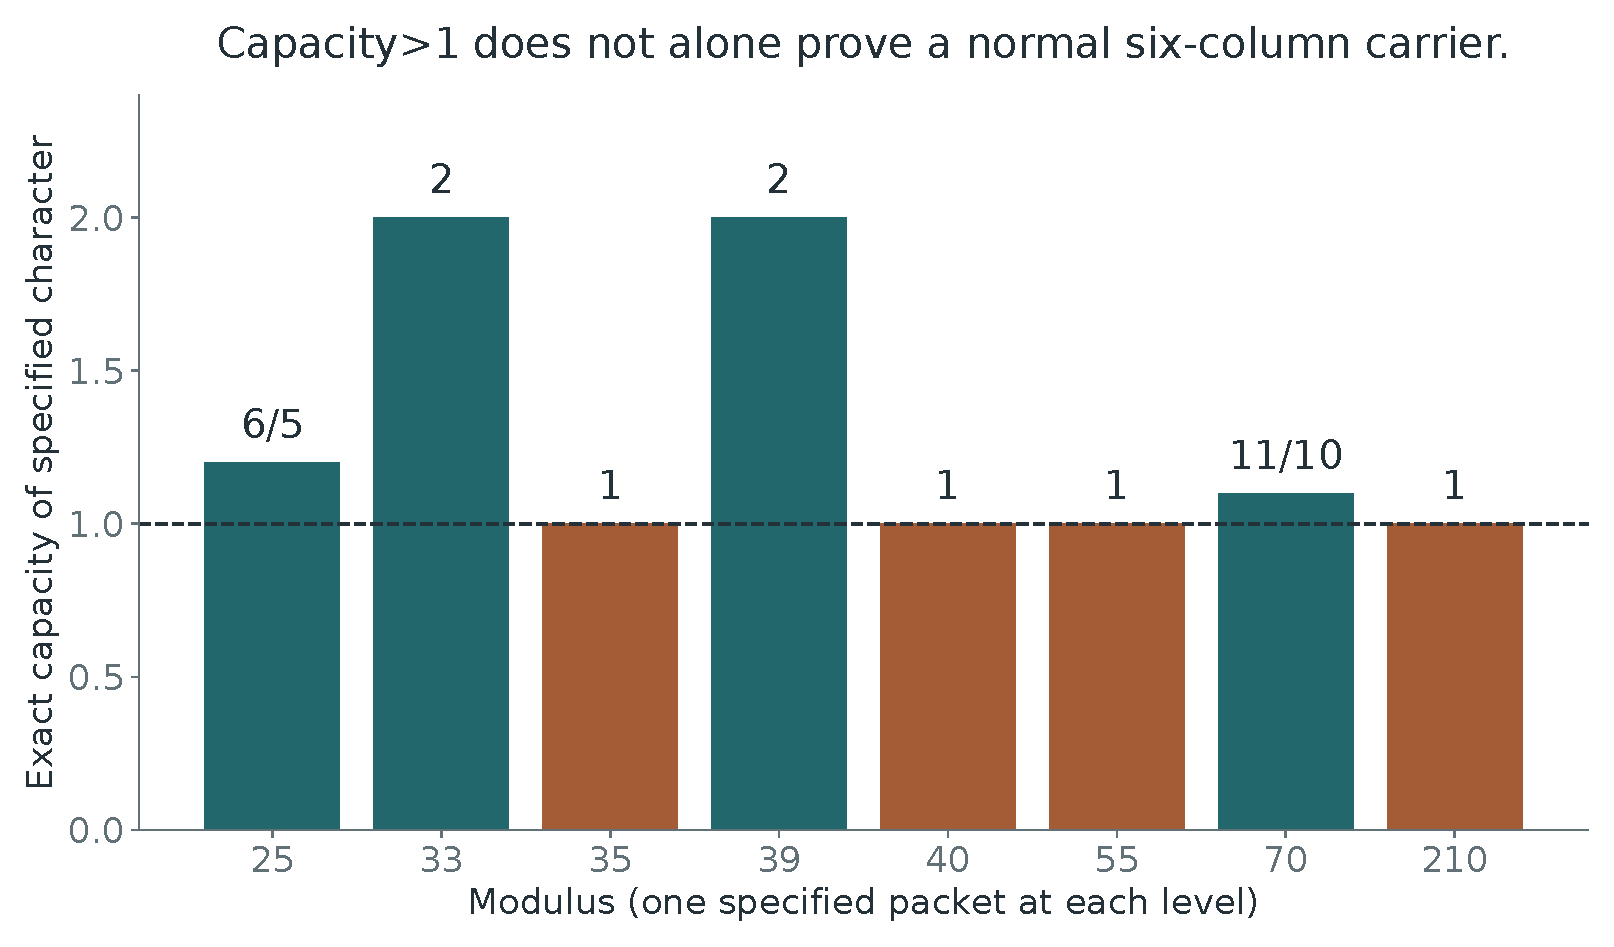
\includegraphics[width=0.98\linewidth]{26_capacity_values.pdf}\caption{Seven named capacity certificates and the degree-210 target. These eight specified characters are not a census of their degrees.}\end{figure}

\hypertarget{capacity_cycles-a-uniform-obstruction-to-universal-matrix-carrier-coverage}{%
\section{A uniform obstruction to universal matrix-carrier
coverage}\label{capacity_cycles-a-uniform-obstruction-to-universal-matrix-carrier-coverage}}

For \(q\ge2\) and \(1\le b<q\), set

\begin{equation}\label{eq:capacity_cycles-3.1}
m=5q,\qquad
 a_{q,b}=(b,b+q,b+2q,b+3q,b+4q,5(q-b)).\end{equation}

\hypertarget{capacity_cycles-lemma-3.1-balance}{%
\subsection{Lemma 3.1: balance}\label{capacity_cycles-lemma-3.1-balance}}

Every character in \eqref{eq:capacity_cycles-3.1} is full support and its rational orbit is of
type \((2,2)\).

Let \(t\) be a unit modulo \(5q\), and let \(b'=tb\bmod q\), with
\(1\le b'<q\). Multiplication by \(t\) permutes the five residues in the
fiber over \(b'\), because \(t\) is a unit modulo 5. The first five
least-positive residues are therefore, in some order,

\[
b',b'+q,b'+2q,b'+3q,b'+4q.
\]

The last residue is \(5(q-b')\). Their sum is \(15q=3m\). This is a
proof for all parameters, separate from the finite checks in the bundle.

\hypertarget{capacity_cycles-no-positive-anticanonical-invariant-column-matrix}{%
\subsection{No positive-anticanonical invariant-column
matrix}\label{capacity_cycles-no-positive-anticanonical-invariant-column-matrix}}

Assume \(q>5\) and \(\gcd(b,q)=1\). For every nonsingular nonnegative
integral matrix \(A\) such that

\[
A^Ta_{q,b}\in5q\mathbf Z^6,
\qquad w=A^{-1}\mathbf1>0,
\]

one has

\begin{equation}\label{eq:capacity_cycles-3.2}
\boxed{\sum_j w_j\le1.}\end{equation}

In fact \(C(a_{q,b})=1\).

\textbf{Proof.} Define

\[
y_q=\frac1q(1,1,1,1,1,q-5),\qquad y_q\cdot\mathbf1=1.
\]

If \(v\in\mathcal L_{a_{q,b}}\), reduction modulo \(q\), followed by
cancellation of the unit \(b\), gives

\[
v_0+v_1+v_2+v_3+v_4-5v_5\equiv0\pmod q.
\]

Hence

\[
N=v_0+v_1+v_2+v_3+v_4+(q-5)v_5
\]

is divisible by \(q\). It is a positive integer because \(v\ne0\) and
\(q>5\). Therefore \(N\ge q\), or \(y_q\cdot v\ge1\). Lemma 2.1 proves
\(C(a_{q,b})\le1\).

Conversely \(v=\mathbf1\) is invariant, because \(\sum a_i=3m\), and
putting weight 1 on it is a feasible point of \eqref{eq:capacity_cycles-2.1}. Thus
\(C(a_{q,b})=1\), proving \eqref{eq:capacity_cycles-3.2}. \(\square\)

The invariant column set is unchanged by multiplying a character by a
unit modulo \(m\), or by replacing \((m,a)\) by \((km,ka)\). A
coordinate permutation merely permutes the columns' entries and the dual
costs. Consequently none of these changes evades the obstruction.

For example, at degree 35 the packet is \((1,8,15,22,29,30)\), and the
dual is \((1,1,1,1,1,2)/7\). No increase in exponent-search bounds can
produce a matrix of the earlier type with normalized weight sum greater
than 1.

\textbf{Interpretation.} This disproves universal applicability of the
specific positive-anticanonical matrix criterion proposed in v0.1.0. It
does not disprove the Hodge conjecture, exclude other uniruled carriers
or correspondences, or exclude non-anticanonical approaches.

\hypertarget{capacity_cycles-an-actual-cycle-for-the-missed-family}{%
\section{An actual cycle for the missed
family}\label{capacity_cycles-an-actual-cycle-for-the-missed-family}}

The construction now bypasses the carrier model entirely.

Fix \(q\ge2\), put \(m=5q\), and choose \(\kappa\in\mathbf C\) with

\[
\kappa^q=-1/5.
\]

Set

\[
z=x_5,\quad t_i=x_i^q\ (0\le i\le4),\quad P=x_0x_1x_2x_3x_4,
\]

and let \(e_j\) be the elementary symmetric polynomial of degree \(j\)
in \(t_0,\ldots,t_4\). Define

\begin{equation}\label{eq:capacity_cycles-4.1}
\boxed{
Z_\kappa=\{e_1=0,\ e_2=0,\ P-\kappa z^5=0\}\subset\mathbf P^5.
}\end{equation}

\hypertarget{capacity_cycles-proposition-4.1-containment-in-the-fermat-fourfold}{%
\subsection{Proposition 4.1: containment in the Fermat
fourfold}\label{capacity_cycles-proposition-4.1-containment-in-the-fermat-fourfold}}

Newton's identity is

\begin{equation}\label{eq:capacity_cycles-4.2}
p_5=e_1(e_1^4-5e_1^2e_2+5e_1e_3+5e_2^2-5e_4)-5e_2e_3+5e_5.\end{equation}

Since \(e_5=P^q\), on \(Z_\kappa\) one has

\[
F_m=p_5+z^{5q}=5P^q+z^{5q}
=(5\kappa^q+1)z^{5q}=0.
\]

Thus \(Z_\kappa\subset X_{5q}\). Its defining equations have degrees
\(q,2q,5\).

\hypertarget{capacity_cycles-proposition-4.2-the-surface-is-an-integral-complete-intersection}{%
\subsection{Proposition 4.2: the surface is an integral complete
intersection}\label{capacity_cycles-proposition-4.2-the-surface-is-an-integral-complete-intersection}}

Let

\[
S_q=\{e_1(x_0^q,\ldots,x_4^q)=e_2(x_0^q,\ldots,x_4^q)=0\}\subset\mathbf P^4.
\]

The coordinate-power map to the \(t\)-space is finite, so the dimension
is two. In characteristic zero, on \(e_1=0\) the equations are
equivalent to

\[
\sum x_i^q=0,\qquad\sum x_i^{2q}=0.
\]

At a hypothetical failure of Jacobian rank, there would be constants
\(\lambda,\mu\), not both zero, such that for each nonzero coordinate

\[
\lambda+2\mu x_i^q=0.
\]

The case \(\mu=0\) is impossible. Otherwise all nonzero \(x_i^q\) equal
the same nonzero constant. Their sum cannot vanish in characteristic
zero. Thus \(S_q\) is smooth. It is a connected complete intersection of
positive-dimensional ample divisors, hence irreducible.

The same argument with four coordinates shows that \(S_q\cap\{x_i=0\}\)
is a smooth reduced complete-intersection curve. Distinct such curves
share no irreducible component, since imposing two coordinate zeros
gives a zero-dimensional intersection. In particular the divisor of
\(P\) has valuation one at the generic point of each coordinate curve.

Forgetting \(z\) defines a finite flat cover \(Z_\kappa\to S_q\) of
degree five. On a chart trivializing \(\mathcal O_{S_q}(1)\), its
equation is \(z^5=P/\kappa\), with the corresponding trivializations
understood. At a generic coordinate curve its right side has valuation
one. The degree-five polynomial is Eisenstein over that discrete
valuation ring and is therefore irreducible over the function field of
\(S_q\). Finite flatness makes the cover generically integral without
vertical or embedded components, locally its monic algebra injects into
the generic field extension. Hence the cover is integral.

The two equations of \(S_q\), followed by the monic equation in \(z\),
form a homogeneous regular sequence. The resulting projective ideal is
saturated and defines the integral complete intersection \eqref{eq:capacity_cycles-4.1}.
Therefore

\[
\dim Z_\kappa=2,\qquad\deg Z_\kappa=q(2q)5=10q^2.
\]

The surface need not be smooth. Villaflor Loyola's complete-intersection
theorem does not impose smoothness of \(Z\), its proof explicitly
reduces to a smooth perturbation. We use this version, not an unverified
smooth-cycle variant.

\begin{figure}[tbp]\centering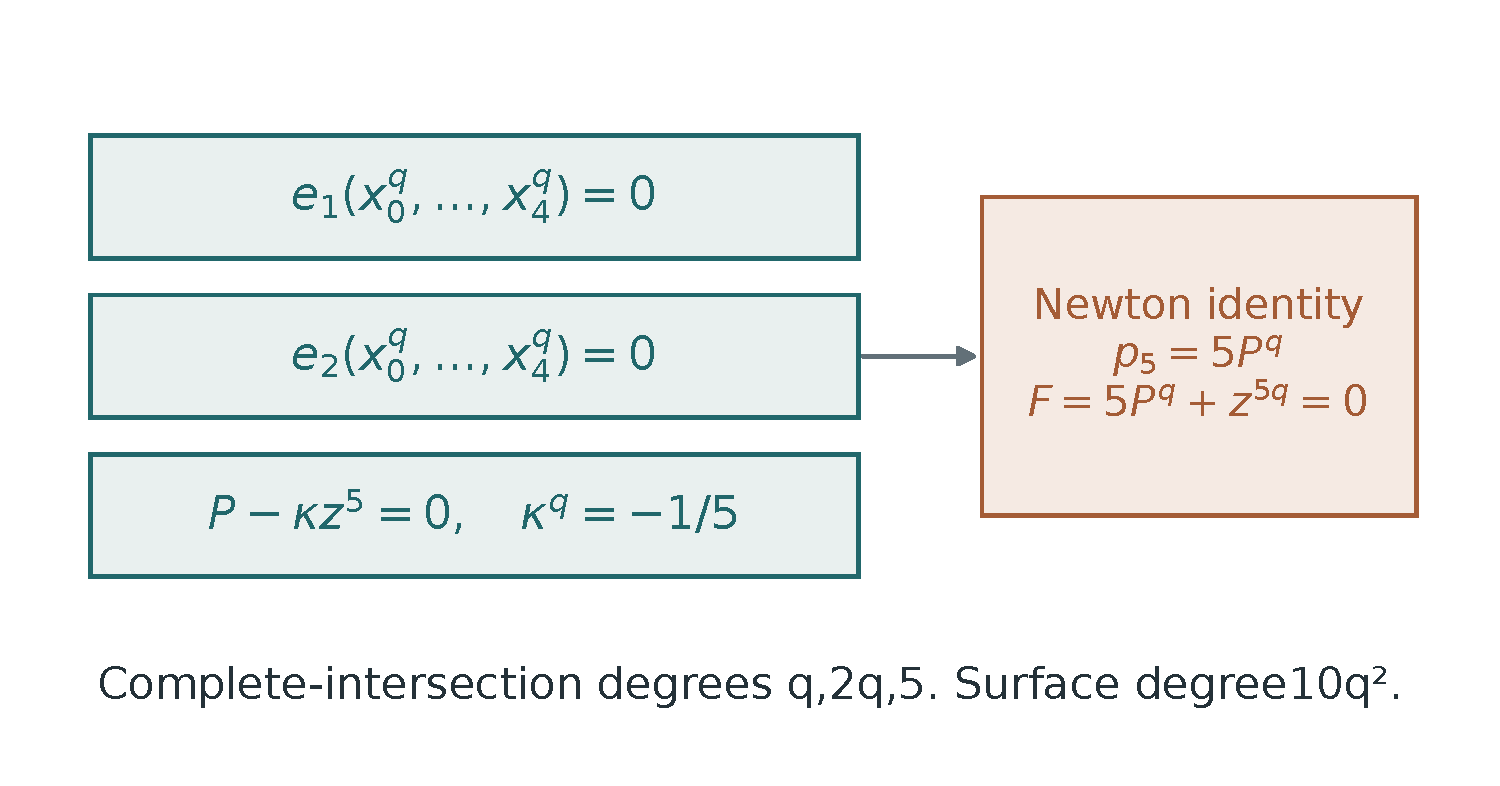
\includegraphics[width=0.98\linewidth]{30_explicit_fivephase_surface.pdf}\caption{A direct reconstruction of the known Aoki standard surface. Containment follows from exact Newton identities.}\end{figure}

\hypertarget{capacity_cycles-the-exact-jacobian-determinant}{%
\section{The exact Jacobian
determinant}\label{capacity_cycles-the-exact-jacobian-determinant}}

Define

\[
\begin{aligned}
f_1&=e_1,&g_1&=e_1^4-5e_1^2e_2+5e_1e_3+5e_2^2-5e_4,\\
f_2&=e_2,&g_2&=-5e_3,\\
f_3&=P-\kappa z^5,&g_3&=5\sum_{j=0}^{q-1}P^{q-1-j}\kappa^jz^{5j}.
\end{aligned}
\]

The geometric-series identity and \eqref{eq:capacity_cycles-4.2} give

\begin{equation}\label{eq:capacity_cycles-5.1}
F_m=f_1g_1+f_2g_2+f_3g_3.\end{equation}

Let

\[
H=(f_1,g_1,f_2,g_2,f_3,g_3),\qquad
D_\kappa=\det\operatorname{Jac}_{(x_0,\ldots,x_4,z)}H,
\]

and

\[
\Delta(t)=\prod_{0\le i<j\le4}(t_i-t_j).
\]

\hypertarget{capacity_cycles-theorem-5.1-uniform-determinant-formula}{%
\subsection{Theorem 5.1: uniform determinant
formula}\label{capacity_cycles-theorem-5.1-uniform-determinant-formula}}

\begin{equation}\label{eq:capacity_cycles-5.2}
\boxed{
D_\kappa=625q^5\Delta(x_0^q,\ldots,x_4^q)
\sum_{b=1}^{q-1}\kappa^{q-b}P^{b-1}z^{5(q-b)-1}.
}\end{equation}

\textbf{Proof.} First,

\begin{equation}\label{eq:capacity_cycles-5.3}
df_1\wedge dg_1\wedge df_2\wedge dg_2
=25\,de_1\wedge de_2\wedge de_3\wedge de_4.\end{equation}

Only the term \(-5de_4\) in \(dg_1\) survives after wedging with
\(de_1,de_2,de_3\), the row permutation has positive sign.

Next, direct differentiation yields

\begin{equation}\label{eq:capacity_cycles-5.4}
df_3\wedge dg_3=
25q\sum_{j=1}^{q-1}\kappa^jP^{q-1-j}z^{5j-1}\,dP\wedge dz.\end{equation}

For each interior index \(j\), the two contributing coefficients add to
\(j+(q-j)=q\). The endpoint terms have zero derivative coefficient. Thus
\eqref{eq:capacity_cycles-5.4} is an identity for every positive integer \(q\), not an
interpolation from checked values.

Finally,

\[
de_1\wedge\cdots\wedge de_5
=\Delta(t)\,dt_0\wedge\cdots\wedge dt_4.
\]

Use \(e_5=P^q\) and
\(dt_0\wedge\cdots\wedge dt_4=q^5P^{q-1}\,dx_0\wedge\cdots\wedge dx_4\).
Cancellation in the polynomial ring gives

\begin{equation}\label{eq:capacity_cycles-5.5}
de_1\wedge\cdots\wedge de_4\wedge dP
=q^4\Delta(x^q)\,dx_0\wedge\cdots\wedge dx_4.\end{equation}

Combining \eqref{eq:capacity_cycles-5.3}, \eqref{eq:capacity_cycles-5.4}, and \eqref{eq:capacity_cycles-5.5}, and putting \(b=q-j\), proves \eqref{eq:capacity_cycles-5.2}.
The identity extends across \(P=0\) because it is a polynomial identity.
\(\square\)

The degree of every monomial in \eqref{eq:capacity_cycles-5.2} is \(15q-6=3m-6\), as required for
a middle residue numerator.

\hypertarget{capacity_cycles-nonzero-periods-not-just-a-formal-character-match}{%
\section{Nonzero periods, not just a formal character
match}\label{capacity_cycles-nonzero-periods-not-just-a-formal-character-match}}

Fix \(1\le b<q\). In the order used in \eqref{eq:capacity_cycles-3.1}, the coefficient of

\begin{equation}\label{eq:capacity_cycles-6.1}
x_0^{b-1}x_1^{b+q-1}x_2^{b+2q-1}x_3^{b+3q-1}x_4^{b+4q-1}
 z^{5(q-b)-1}\end{equation}

in \(D_\kappa\) is

\begin{equation}\label{eq:capacity_cycles-6.2}
625q^5\kappa^{q-b}\ne0.\end{equation}

All permutations of the first five exponents have the same nonzero
magnitude, with the Vandermonde sign. Different values of \(b\) and
different permutations give different monomials. Every exponent lies
between zero and \(m-2\), so no term is killed by the Fermat Jacobian
ideal.

Define the dual numerator

\begin{equation}\label{eq:capacity_cycles-6.3}
Q_b=\prod_{i=0}^5x_i^{m-a_{q,b,i}-1}.\end{equation}

It has degree \(3m-6\). Because the product \(Q_bD_\kappa\) has socle
degree, a surviving monomial modulo \(J_{F_m}\) must have all six
exponents equal to \(m-2\). Formula \eqref{eq:capacity_cycles-6.1} is the unique term with this
complement. Therefore

\begin{equation}\label{eq:capacity_cycles-6.4}
Q_bD_\kappa\equiv625q^5\kappa^{q-b}S_m\pmod{J_{F_m}}.\end{equation}

For the Fermat polynomial,

\[
\det\operatorname{Hess}(F_m)=[m(m-1)]^6S_m.
\]

Apply Villaflor Loyola's Theorem 1.2 with dimension four and the
ordering fixed above. Its constant is

\[
c=\frac{625q^5\kappa^{q-b}}{[m(m-1)]^6}.
\]

The exact period is consequently

\begin{equation}\label{eq:capacity_cycles-6.5}
\boxed{
\int_{Z_\kappa}\operatorname{res}\left(\frac{Q_b\Omega}{F_m^3}\right)
=\frac{(2\pi i)^2}{50q}\,\kappa^{q-b}\ne0.
}\end{equation}

The normalization follows from \(625q^5/[2(5q)^6]=1/(50q)\). In
conventions using a differently normalized residue map, the displayed
constant changes with that convention, nonvanishing does not.

\hypertarget{capacity_cycles-rational-algebraicity-of-whole-packets}{%
\subsection{Rational algebraicity of whole
packets}\label{capacity_cycles-rational-algebraicity-of-whole-packets}}

Let \(h\) denote the hyperplane class. Since \(\deg Z_\kappa/m=2q\), the
primitive part

\[
\xi_\kappa=[Z_\kappa]-2q h^2
\]

is rational and algebraic. Villaflor Loyola's Theorem 1.1 identifies its
primitive residue numerator with \(-2D_\kappa/m\). Thus its complex
eigenspace support consists of exactly the \(120(q-1)\) characters
obtained from \eqref{eq:capacity_cycles-3.1} by permuting the first five entries and varying
\(b\).

That set is closed under multiplication by units modulo \(m\), by Lemma
3.1. Each of its eigenspaces has dimension one. The
\(\mathbf Q[G_m]\)-submodule generated by \(\xi_\kappa\) therefore has
complexification equal to the entire sum of those eigenlines: applying
the complex character idempotents isolates each nonzero component. Since
the generator and the group action are rational, this is the
complexification of the claimed rational submodule.

Every vector in that rational submodule is a rational linear combination
of classes of diagonal translates of \(Z_\kappa\) and of \(h^2\). Hence
every rational packet in the family is algebraic. Its rational algebraic
subspace has dimension

\[
120(q-1)
\]

for this fixed choice of the last coordinate. This is not the dimension
of all Hodge classes on \(X_{5q}\).

The conclusion recovers Aoki's standard family, including the elementary
decomposable midpoint case at even levels. It does not close arbitrary
nonstandard five-primary packets.

\hypertarget{capacity_cycles-a-concrete-example-at-degree-35}{%
\section{A concrete example at degree
35}\label{capacity_cycles-a-concrete-example-at-degree-35}}

Take \(q=7\), \(b=1\), \(\kappa^7=-1/5\). Then

\[
a=(1,8,15,22,29,30),\quad
Z_\kappa=\left\{
\begin{array}{l}
\sum_{i=0}^4x_i^7=0,\\
\sum_{0\le i<j\le4}x_i^7x_j^7=0,\\
x_0x_1x_2x_3x_4=\kappa x_5^5
\end{array}\right\}\subset X_{35}.
\]

The cycle has degree 490. The rational packet has dimension
\(\varphi(35)=24\), since its first character entry is 1. The
determinant coefficient is

\[
10,504,375\,\kappa^6.
\]

For

\[
Q_1=x_0^{33}x_1^{26}x_2^{19}x_3^{12}x_4^5x_5^4,
\]

one obtains

\[
\boxed{
\int_{Z_\kappa}\operatorname{res}\left(\frac{Q_1\Omega}{F_{35}^3}\right)
=\frac{(2\pi i)^2\kappa^6}{350}\ne0.
}
\]

At the same time, the uniform matrix-obstruction theorem above proves
that this packet has capacity exactly 1 and cannot use the
positive-anticanonical matrix route. Thus this is an explicit example
where failure of that constructor is compatible with, and bypassed by,
an actual algebraic cycle.

At degree 70 the standard packet \((1,15,29,43,57,65)\) obtained by
setting \(q=14\) is \textbf{different} from the earlier packet
\((1,20,24,42,61,62)\). Their capacities are respectively 1 and
\(11/10\). They must not be conflated.

\begin{figure}[tbp]\centering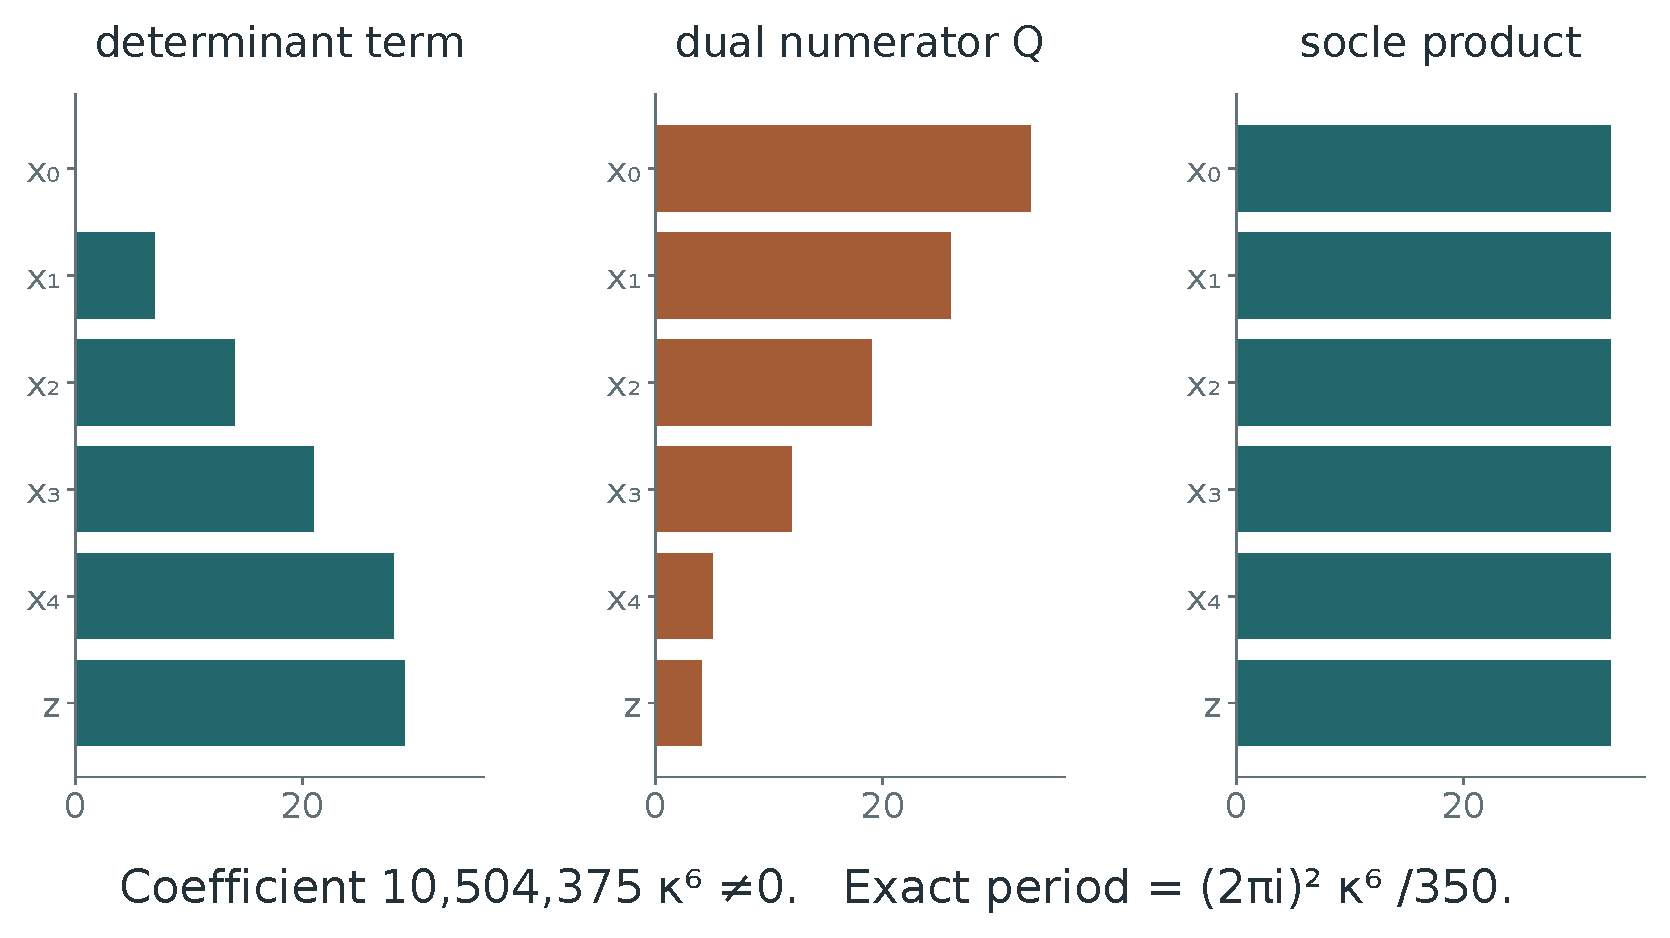
\includegraphics[width=0.98\linewidth]{31_socle_pairing35.pdf}\caption{At degree 35 the exact socle coefficient gives a nonzero period and a genuine packet component.}\end{figure}

\hypertarget{capacity_cycles-exact-computations-and-limitations}{%
\section{Exact computations and
limitations}\label{capacity_cycles-exact-computations-and-limitations}}

The final verifier uses integers, rational numbers, and symbolic
polynomial identities. It uses no floating-point arithmetic, random
sampling, network request, or optimization routine.

Its 137 grouped assertions include:

\begin{itemize}
\tightlist
\item
  balance and exact primal/global-dual certificates for seven specified
  packets,
\item
  the predecessor archive checksum,
\item
  Newton's identity and the elementary-symmetric Jacobian identity,
\item
  exact six-by-six intermediate determinants for \(q=2,3,4,5,7,11,17\),
\item
  independent socle-pairing checks for every \(b\) at \(q=2,7,11\),
\item
  all \(b\), all units, and all first-five permutations for
  \(2\le q\le64\), totaling 241,920 distinct support monomials and
  218,836 balance/conjugacy instances.
\end{itemize}

The seven globally certified capacity values are:

\begin{longtable}[]{@{}lll@{}}
\toprule\noalign{}
Modulus & Character & Capacity \\
\midrule\noalign{}
\endhead
\bottomrule\noalign{}
\endlastfoot
25 & (1,6,11,16,20,21) & 6/5 \\
33 & (1,4,16,22,25,31) & 2 \\
35 & (1,8,15,22,29,30) & 1 \\
39 & (1,7,16,22,34,37) & 2 \\
40 & (1,9,17,25,33,35) & 1 \\
55 & (1,12,23,34,45,50) & 1 \\
70 & (1,20,24,42,61,62) & 11/10 \\
\end{longtable}

These are seven specified inputs, not a census of all characters at
those levels. Capacities 2 in the table do not themselves supply a
six-column normal carrier.

The finite identities support the implementations. The all-parameter
assertions come from the separate mathematical proofs in the balance,
cycle and period arguments above, conditional only on the stated
standard algebraic-geometric and residue theorems. These proofs remain
at manuscript level.

\hypertarget{capacity_cycles-unclosed-targets}{%
\subsection{Unclosed targets}\label{capacity_cycles-unclosed-targets}}

No proof is given of the general Hodge conjecture, of coverage of every
Fermat packet, of the full CM half-twist Chow correspondence, or of the
earlier central-defect realization lemma. The universal
positive-anticanonical invariant-matrix conjecture is false by the
uniform matrix-obstruction theorem above and should not remain in a gap
ledger as an unproved plausible universal lemma.

The usable research architecture is now a collection of separately
certified constructors: carrier transfer where its hypotheses hold,
explicit standard surfaces where the capacity barrier is 1, and other
correspondences for packets not handled by either route. A proof that
such constructors exhaust all Hodge classes is still missing.

\compactpart{Part XII. Weil classes and the failed counterexample route}
\chapter{Explicit Weil classes and a failed counterexample route}
The separate September 22 computation addresses an abelian sixfold of Weil type. Its role is different from the Fermat constructive work. It began by looking for a Hodge class whose chosen geometric representative would fail to deform. The exact calculation found such a failure for a particular graph, then found replacement divisor factorizations. The tested route did not establish nonalgebraicity.

This chapter records the rational classes, the cycle projector, the seed graph, the tangent calculation, the degeneration boundary and the replacement factorization. Every claim is made at the level supported by those objects. The 924-basis calculation is finite exterior algebra. A search over all algebraic cycles was not performed.

\section{The lattice, polarization and seed}
Let $K=\Q(i)$ and take homology lattice $\Z[i]^6$. Use the conjugate-linear-first Hermitian form
\[
h(v,w)=\overline v^{\,t}\operatorname{diag}(1,1,1,-1,-1,-3)w,
\qquad E=\Im h.
\]
The seed complex structure is
\[
J_0=\operatorname{diag}(i,i,i,-i,-i,-i).
\]
It preserves the alternating form $E$, and $E(v,J_0v)>0$ for nonzero $v$. These are the Riemann positivity conditions for the seed abelian variety. The sign depends on the declared Hermitian convention. Omitting that convention would leave the polarization claim ambiguous.

Write $(x_1,y_1,\ldots,x_6,y_6)$ for the integral dual basis. Define
\[
\Omega_6=\bigwedge_{j=1}^{6}(x_j+iy_j),\qquad
u=\Re\Omega_6,\qquad v=\Im\Omega_6.
\]
Both $u$ and $v$ are explicit integral six-forms, with 32 nonzero terms each. An unspecified complex determinant-line generator would not by itself define these rational classes. The chosen expansion removes that ambiguity.

For complex structures in the Weil domain with three positive and three negative $K$-embedding directions, $\Omega_6$ has type $(3,3)$. Indeed, the $K$-determinant contains three one-forms from each Hodge side. Thus the rational span
\[
W=\Span_{\Q}\{u,v\}
\]
is a Hodge substructure of degree six across the domain. The first-order computation confirms that persistence in all 18 real tangent directions at the seed. The all-domain assertion comes from the determinant Hodge-type argument, rather than extrapolation from those tangent tests.

\section{The intersection form and primitive directions}
Use the orientation
\[
\int x_1y_1\cdots x_6y_6=-1
\]
for this seed. If $\theta$ is the polarization class specified by $E$, the exact Gram matrix on $(\theta^3,u,v)$ is
\[
\begin{pmatrix}
2160&0&0\\
0&-32&0\\
0&0&-32
\end{pmatrix}.
\]
The exterior calculation also gives $\theta\wedge u=\theta\wedge v=0$, so the two Weil directions are primitive. The negative signs are compatible with the middle-degree Hodge--Riemann convention and the stated orientation.

For any class $c$ in degree six, the orthogonal projection onto $W$ under this intersection pairing is
\begin{equation}\label{eq:weilprojection}
P_W(c)=-\frac{\langle c,u\rangle u+\langle c,v\rangle v}{32}.
\end{equation}
The verifier checked this identity on every one of the $\binom{12}{6}=924$ rational exterior basis vectors. Its output has image of dimension two, with image basis $u,v$. This is an exact finite-dimensional statement.

\section{An algebraic projector from isogenies}
An arbitrary orthogonal projector need not be algebraic. In this example the desired projector can be written as a rational polynomial in actual isogeny pullbacks.

Let
\[
S=[2+i]^*+[2-i]^*
\]
act on $H^6$. The exact eigenvalues and dimensions are
\[
\begin{array}{c|rrrr}
\text{eigenvalue}&-234&-70&150&250\\
\text{dimension}&2&72&450&400 .
\end{array}
\]
Their dimensions sum to 924. The eigenvalue $-234$ selects $W$, because
\[
(2+i)^6=-117+44i,\qquad
(2-i)^6=-117-44i.
\]
The rational polynomial
\begin{equation}\label{eq:weilisogeny}
P_W=\frac{(S+70I)(S-150I)(S-250I)}{-30480384}
\end{equation}
equals \eqref{eq:weilprojection}. The denominator is the product of the three eigenvalue differences at $-234$. It is nonzero, and the polynomial takes value one on $W$ and zero on the other three eigenspaces.

The maps $[2\pm i]$ are algebraic endomorphisms of the abelian variety. Their graphs induce the pullback operators. Hence \eqref{eq:weilisogeny} preserves rational algebraic cycle classes. A nonzero $P_W$ component of any algebraic threefold supplies an algebraic Weil direction, even if the original effective cycle has a large ambient component.

This also corrects a source-level eigencharacter confusion. The polarization cube has eigenvalue
\[
[2+i]^*(\theta^3)=125\,\theta^3=\operatorname{Norm}(2+i)^3\theta^3,
\]
while the Weil directions have eigenvalues $-117\pm44i$. The norm-cubed character therefore identifies the polarization cube, and does not identify the two-dimensional Weil subspace. The September audit recorded this local failure in Section 4.3 of the cited secant-cycle preprint. That specific calculation is not a full audit of the preprint \cite{SecantPreprintAudit}.

\section{The seed graph supplies both rational Weil classes}
At the seed, take the graph of
\[
(z_1,z_2,z_3)\longmapsto
(z_1,z_2,z_3,\overline z_1,\overline z_2,\overline z_3).
\]
Conjugation preserves the $\Z[i]$ lattice and is holomorphic from an elliptic factor with complex structure $i$ to a target factor with complex structure $-i$. Thus this map defines an abelian-subvariety graph and is algebraic at $J_0$. On its three source factors the polarization restricts to weights $(2,2,4)$, giving $\int_Z\theta^3=3!\cdot2\cdot2\cdot4=96$. Pulling the explicit determinant form back to the graph gives the other two periods. In full,
\[
\left(\int_Z\theta^3,\int_Zu,\int_Zv\right)=(96,0,-8).
\]
Its exact Poincaré dual has 64 nonzero basis terms. Pairing that dual against all 924 basis vectors reproduces the graph periods. The projector gives
\[
P_W[Z]=v/4.
\]
The isogeny $[1+i]$ acts on the Weil directions by
\[
[1+i]^*u=8v,\qquad[1+i]^*v=-8u.
\]
It follows that
\[
v=4P_W[Z],\qquad
u=-\tfrac12[1+i]^*P_W[Z].
\]
Thus both directions are algebraic at this seed, through rational combinations of actual graph and isogeny correspondences.

The class $v$ is primitive. It need not be the class of a single effective threefold. For a nonzero effective codimension-three cycle on a polarized sixfold, its pairing with $\theta^3$ is positive. A primitive $v$ has pairing zero. The correct target permits signed rational cycles, or asks for a nonzero projection of an arbitrary effective cycle. Looking for a Chow component whose individual effective members equal $v$ would impose the wrong problem.

\section{A representative can obstruct without obstructing its class}
The Weil domain has real tangent dimension 18 at the seed. For the selected graph, the first-order graph-preservation constraints have real rank 12 in the nonsplit case with weights $(1,1,3)$. The graph-preserving tangent space therefore has real dimension 6, or complex dimension 3.

The split control with weights $(1,1,1)$ has constraint rank 6, leaving real dimension 12, or complex dimension 6. These ranks were checked both in the exterior calculation and by a separate exact real matrix construction.

\begin{figure}[tbp]
\centering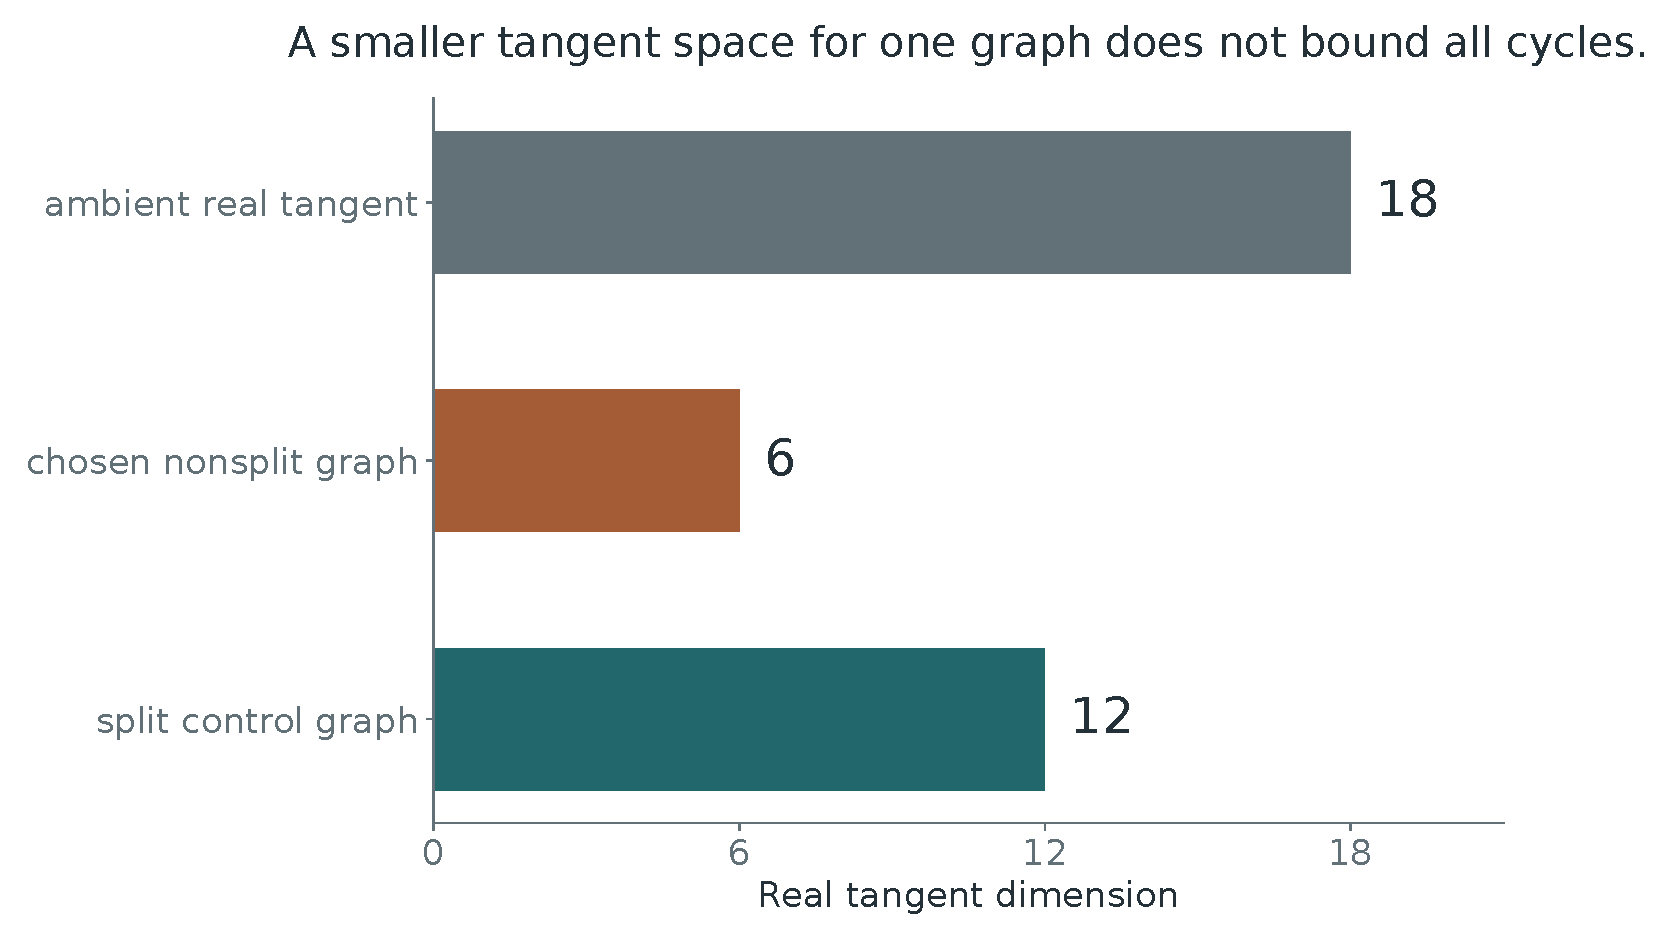
\includegraphics[width=0.98\linewidth]{33_weil_graph_tangent_boundary.pdf}
\caption{Exact tangent dimensions for one selected graph at two seeds. These ranks do not bound deformation spaces of every algebraic cycle.}
\end{figure}

The nonsplit graph fails to follow many nearby Weil directions, even though $u,v$ remain Hodge classes. This is a failure of that geometric representative. It does not show that every cycle representing the same rational class fails, and it does not bound all components of a Chow variety.

To prove a Hodge counterexample one would need a global statement that every algebraic threefold has zero pairing with both $u$ and $v$ at some fully mixed member, while those rational Hodge classes remain nonzero. A tangent rank bound for one graph provides no such statement.

\section{The product locus and replacement factorizations}
Split the six directions into a four-dimensional Weil factor $C$ and a two-dimensional factor $B$. The determinant forms factor:
\[
\Omega_6=\Omega_C\wedge\Omega_B.
\]
Writing their real and imaginary parts as $c_R,c_I,b_R,b_I$ gives
\[
u=c_Rb_R-c_Ib_I,\qquad
v=c_Rb_I+c_Ib_R.
\]
On the product locus, the degree-four Weil classes on $C$ are algebraic by the checked fourfold theorem, and the degree-two classes on $B$ are divisors by Lefschetz $(1,1)$. Their products give the degree-six classes. This locus has complex dimension five. The product argument does not establish the fully mixed sixfold statement \cite{MarkmanWeil,MarkmanICM2026}.

The selected mixed tangent direction $B_{13}=1$ breaks the original factorization infinitesimally: the old surface factor loses type $(1,1)$ and the old fourfold factor loses type $(2,2)$. Nevertheless the full $u,v$ remain type $(3,3)$. At first this looked like a promising obstruction.

The exact audit then found replacement divisor factors using the pairs
\[
(1,6),\qquad(2,5),\qquad(3,4).
\]
These replacement factors remain of divisor type along the selected tangent. With
\[
X=-\tfrac12(\Delta J)J_0,\qquad
J(t)=e^{tX}J_0e^{-tX},
\]
the pair blocks are preserved by the integrating generator. Thus the alternate factorization defeats the tested counterexample path. It proves no universal result for every fully mixed point, and it invalidates the inference that failure of the original factorization establishes nonalgebraicity.

\section{The nilpotent does not construct a degeneration}
The exact computation also produced a nilpotent in the unitary Lie algebra, with block
\[
i\begin{pmatrix}1&-1\\1&-1\end{pmatrix}
\]
on each of the pairs $(e_1,e_4)$ and $(e_2,e_5)$. It has square zero, rank two over $K$ and rank four over $\Q$. The remaining Hermitian plane is $\operatorname{diag}(1,-3)$.

Modulo 3, the equation $x^2+y^2=0$ has only the solution $(0,0)$. This is a finite anisotropy control for the residual discriminant. It does not construct a semistable algebraic family with this nilpotent as monodromy. An abstract rational nilpotent satisfying Lie-algebra identities is weaker than a geometric degeneration with the required integral, polarization and admissibility data.

The earlier source audit quoted Brosnan's Proposition 4 as a constraint relating maximal degeneration to split discriminant. The current audit authenticated the paper metadata but did not re-extract that exact proposition. This reader therefore retains the implication as a conditional literature context, and does not use it to prove nonalgebraicity \cite{BrosnanDegeneration}. Even a verified obstruction to one maximal degeneration would not exclude all algebraic cycle constructions.

\section{The remaining question}
For a fully mixed member of this discriminant-$-3$ Weil family, does there exist an algebraic threefold $Z$ such that
\[
\left(\int_Zu,\int_Zv\right)\ne(0,0)?
\]
One such nonzero period, followed by the algebraic projector and the $[1+i]$ action, would generate both Weil directions. The tested graph is one source at the seed. The product and replacement factorization give additional sources on special loci. Exhausting every fully mixed member is a separate task.

The checked Markman results cover abelian fourfolds of Weil type and the stated split or discriminant-$-1$ sixfold cases. They are not silently extended to the nonsplit discriminant-$-3$ sixfold considered here. The source contracts retain these hypotheses explicitly.

The Weil audit closes a particular counterexample attempt with a failure record. It supplies exact rational classes, an algebraic projector, algebraic seeds and clear constraints on deformation arguments. It does not produce a Hodge counterexample, establish a rank bound for all cycles, or prove the general conjecture.

\compactpart{Part XIII. Reproduction, corrections and remaining obligations}
\chapter{What the exact replay verifies}
The purpose of the evidence bundle is to make each finite claim independently inspectable. The final result is not a single undifferentiated pass flag. It is a collection of named inputs, arithmetic domains, frozen certificates, execution records and logical boundaries.

The proof-critical September verifiers use integers, rational numbers and exact symbolic polynomial rings. Discovery used bounded enumeration and optimization where helpful. The discovered certificates were accepted only after exact replay. A floating-point optimizer's successful status is not the final proof object.

\section{The current finite contract}
\begin{longtable}{p{0.25\linewidth}p{0.22\linewidth}p{0.43\linewidth}}
\toprule
Evidence layer & Fresh result & Mathematical boundary\\
\midrule
Degree-70 carrier & 24 grouped checks passed & Matrix, character, weighted degree, coordinate strata and radical ideal identities. The geometry uses classical inputs.\\
Degree-210 transfer & 46 grouped checks passed & All target/source conjugates, signed identity, standard blocks, stabilizing pairs and dual premise.\\
Capacity and cycles & 137 grouped assertions passed & Seven exact capacities, symbolic determinant controls and the specified cycle support range.\\
Five-phase supports & 241,920 monomials & All $b$, all first-five permutations, and $2\le q\le64$. Distinct from all Fermat packets.\\
Five-phase balance & 218,836 instances & The retained finite parameter and unit-conjugacy range. Uniformity uses a separate proof.\\
K23 reconstruction & 364 certificates & Generated independently from every valid phase pair and ordered unit conjugate of seven retained inputs.\\
K23 ages & 8,336 comparisons & Exact Hodge-age and opposite-CM-sign checks on those regenerated certificates.\\
Dyadic census & Moduli $8,16,32,64,128$ & The complete finite packet census and implemented grammar at those moduli.\\
Dyadic weighted identity & 87,376 coefficients & Fresh range $3\le s\le9$. The historical larger range was not fully replayed.\\
Weil exterior algebra & 924 basis vectors & Rational projector, intersection pairing and Poincaré-dual identities. No cycle-space census.\\
Projector toy models & 18 tolerance checks & Floating-point illustrations with declared tolerances, and not exact variety-level certificates.\\
\bottomrule
\end{longtable}

These counts are grouped assertions or enumerated instances. They are not counts of independent geometric theorems. Several assertions check different consequences of one frozen certificate, which is appropriate for detecting implementation errors and should not be inflated into independent proof multiplicity.

\section{What changed in the K23 replay}
The archived K23 verifier read the retained certificate JSON and checked its fields. The October audit independently rebuilt the phase grammar from the original rational packet addresses. For each unit conjugate it enumerated valid complementary mod-5 phase pairs, checked the nonzero residual entries, formed the curve, surface and lower-curve blocks, and compared Hodge ages.

The resulting counts by retained packet were
\[
40,\quad60,\quad48,\quad48,\quad48,\quad48,\quad72,
\]
which total 364. This stronger bounded replay guards against a certificate file whose generator omitted or misclassified a valid case. It still covers only the seven declared inputs. It neither proves the universal mixed-conductor grammar nor constructs a Chow correspondence.

\section{Why the degree-210 dual is global}
The dual uses numerator vector $(31,87,57,101,84,60)$ and denominator 420. For invariant nonnegative columns of degrees 1 through 13, the exact enumerator checks all 27,131 compositions. Exactly 143 satisfy the congruence, and each has dual numerator at least 420.

For degree at least 14, every coordinate cost is at least 31, so the numerator is at least $14\cdot31=434>420$. Thus the finite premise and the uniform tail cover every nonzero invariant column. The global impossibility statement is proved by this argument, rather than extrapolated from the degree-18 search.

A separate residue-graph calculation finds the same minimum nonempty return cost 420. The independent implementation helps detect an enumeration mistake. The direct finite inequalities and the tail bound remain the stated certificate.

\section{Why the capacity certificates are global}
The seven capacities are proved by matching a feasible primal representation with an exact rational dual. An integer potential on the finite residue graph verifies every edge inequality and every last-edge lower bound. Any nonempty zero-sum word decomposes into a prefix and a last edge. Those inequalities therefore bound every invariant column, at arbitrary degree.

The potential proof does not assume the correctness of the algorithm used to discover the potential. Once the finite inequalities are verified, its argument is a finite sum. The primal representation proves equality at the claimed value. A relaxed capacity optimizer may use fewer than six columns, so equality of capacity does not supply a nonsingular carrier matrix or normal projective geometry.

\section{Uniform formula versus finite benchmark}
The five-phase determinant formula is proved by wedge products and polynomial identities for every positive integer parameter in its stated range. Finite determinants at $q=2,3,4,5,7,11,17$ independently test the implementation and row sign. Socle pairing is separately checked for every $b$ at $q=2,7,11$.

The dyadic identity similarly has a displayed coefficient derivation. Its fresh finite replay checks a bounded range. The later all-degree tree classification is a distinct manuscript proof. Selected independent reconstruction in this edition found no concrete contradiction in its basis/tree/coarea argument once the odd-character nonvanishing leaf was authenticated. That selected review does not silently reverse the August 15 publication-status downgrade. A full uniform write-up and correspondence-level account remain explicit obligations.

\section{Reproduction commands and arithmetic}
The evidence directory includes a portable driver for the bounded replay. Its manifests declare inputs, expected mathematical values, code hashes and arithmetic domains. The driver was tested. The latest exact verifiers need the Python standard library for the transfer and exact symbolic dependencies for the cycle/gradient calculations.

The preserved discovery scripts can take different times, produce a different valid support, or fail to terminate within the same time allowance on another solver version. None of these outcomes invalidates replay of the retained frozen identity. A newly discovered identity requires its own exact residue equality, balance checks and geometric-factor proof.

Replaying a report changes its execution timestamp and output hash. It does not change the frozen character input, matrix, polynomial identity or expected rational value. File checksums identify the exact artifacts used in each recorded run, and the bundle keeps historical sources separate from current replay outputs.

\chapter{Corrections, failures and retractions}
Research progress here includes removing false implications. The negative records identify a failed method or inference, and they do not become counterexamples to the Hodge conjecture.

\section{A positive compressed Gram matrix is insufficient}
The original August cycle-frame theorem asserted that positivity of a compressed frame on a target subspace implied that the cycles spanned that subspace. Without containment or a suitable invariant restriction, this is false.

Take $V=\Span_{\R}\{e_1\}$ in $\R^2$ and let the only cycle vector be $c=e_1+e_2$. Then
\[
S=cc^t=\begin{pmatrix}1&1\\1&1\end{pmatrix}.
\]
The compressed Gram matrix on $V$ is the positive $1\times1$ matrix $(1)$, while $e_1$ does not belong to $\Span(c)$. Positivity proves that the target direction is detected, not that synthesis returns it inside the original cycle span.

The corrected theorem requires $c_j\in V$, obtainable through an explicitly algebraic rational packet projector when available. Without that condition, the exact containment test is
\[
\rank_{\Q}[C\ H_{\Q}]=\rank_{\Q}C.
\]
A rational target basis $H_{\Q}$ is distinct from an orthonormal real basis, since orthonormalization can introduce irrational entries. The old source is preserved unchanged and this correction governs the current reader.

\section{The universal direct matrix constructor is false}
The invariant-column positive-anticanonical matrix criterion was a useful search target. It is not a universal theorem for balanced Fermat packets. The infinite five-phase family has capacity exactly one for the stated coprime parameters, so no matrix of that type can have normalized weight sum greater than one.

The degree-210 target has its own exact capacity-one dual. Yet the signed transfer makes it algebraic under the degree-70 carrier proof and classical operations. Thus positive transfer and negative matrix obstruction coexist on the same packet. Universal applicability of the direct constructor should be removed from a plausible-gap list and replaced by the proved method limitation.

\section{A parameterized weight sum did not identify a new packet family}
An exploratory modification replaced the exponent 7 in the old carrier matrix by a parameter. The formal normalized weights remained positive and summed to $1+7/(10q)$. That calculation alone did not verify a desired full-support character on the projective quotient. It established no uniform new primitive-packet family.

The missing step was character covariance and deck invariance for the claimed target, together with normality and boundary control for the resulting family. The positivity calculation is retained as exploration and is not promoted to a Hodge theorem.

\section{An invalid exploratory input}
The exploratory modulus-45 tuple
\[
(1,10,19,28,36,37)
\]
has sum 131, whereas a middle-balanced six-tuple at that modulus must sum 135. It is not even an admissible starting Hodge character. Its reported candidate capacity $34/45$ is therefore not a Hodge result.

The invalid record remains in the historical discovery evidence and is excluded from the seven authoritative capacity inputs. The exact verifier checks every unit-conjugate sum before accepting a capacity claim. The general lower bound $C(a)\ge1$ for a balanced character also flags the erroneous subunit value.

\section{Bounded search failures are inconclusive}
The atomic chain/loop family failed to find the degree-70 carrier, and an early Hermite-normal-form membership experiment exceeded its 20-second allowance without a conclusion. The later bounded mixed-integer discovery succeeded and was followed by exact replay.

Bounded degree-18 matrix scans failed on selected targets. Those failures alone do not prove global infeasibility. Only the targets covered by the exact dual certificate or the symbolic infinite-family proof have the stated global obstruction.

\section{The five-phase cycles were already known}
The explicit $Z_\kappa$ equations recover the Aoki standard family. The October source audit obtained the original article and checked that its elementary-symmetric construction becomes these equations through Newton identities. A direct determinant and period recomputation is valuable reproducible work, and is not a newly solved open Hodge family.

The earlier retrieval failure is preserved in the archive. It no longer justifies leaving the equations' historical overlap unspecified in this edition. No priority is claimed for the construction, algebraicity or determinant.

\section{The Weil graph failure was defeated}
A first-order obstruction to deforming the original graph does not bound every representative of the same class. The exact audit found replacement divisor factors along the selected mixed direction. Those factors defeat the tested counterexample path.

No nonalgebraicity was proved. The abstract nilpotent was not realized as an algebraic semistable degeneration, and a pointwise tangent rank for one graph was not extended to all cycle-space components. These are distinct missing premises, and none is hidden behind the pass status of the exterior algebra.

\section{Formal source inspection is not a compiler pass}
The current Lean attempt was blocked before elaboration. The restored compiler reported that it failed to locate its application, and the Mathlib files were unavailable. No fresh Lean pass is claimed.

Even a successful compilation of the preserved source would verify only its definitions and hypotheses. The final theorem assumes the algebraic seed and closure rules through an abstract predicate. It does not prove those geometric hypotheses. The current report separates finite arithmetic scripts, assumed closure operations and absent Chow realizations.

\chapter{The live research obligations}
The general Hodge conjecture remains open in this reader. The different missing implications are stated separately because solving one would not automatically solve the others.

\section{Arbitrary smooth projective varieties}
The real obstruction projector vanishes exactly when the algebraic and rational Hodge spaces agree. It provides no algorithm for computing the complete algebraic space. A finite cycle family, actual cohomology coordinates and an exact spanning certificate would close a specified $(X,p)$ case.

An alternative is an explicitly algebraic divisor-lowering transfer with proved packet preservation and invertibility. Its polarized adjoint is an additional algebraicity hypothesis. The cohomological transpose under a chosen metric cannot simply be declared a Chow correspondence.

The analytic branch requires vanishing of the complete finite obstruction $\Phi$, after the proposed stabilization. The range contraction solves only the range equation. Hodge-type Chern characters or trace moments do not force an endomorphism-valued defect to vanish.

\section{Uniform Fermat grammar coverage}
The exact balanced residue equation is available at every degree. The present constructive grammar admits many packets, and finite audits describe the retained degree range. A proof that every full-conductor balanced packet is admitted by one of its channels is still required.

Mixed-conductor Kummer patterns observed in a finite table cannot supply that universal premise. A correctly typed nonzero CM map for every currently admitted K23 case would solve those cases. It would not prove that arbitrary residual packets have that K23 form.

\section{The typed Chow bridge}
Before stating a rank-one isomorphism, fix the coefficient field, the diagonal character projector, the rational Galois orbit and any multiplicities caused by conductor reduction. Construct an actual algebraic kernel and prove a nonzero period or intersection coefficient.

Matching CM types is an identification at Hodge level. The rational tensor can contain off-diagonal embeddings and need not have the dimension of the lower curve factor. These typing requirements belong to the target, rather than editorial details after a claimed proof.

\section{The special constructions}
The degree-70 carrier argument and degree-33 torus/cubic argument remain manuscript geometric constructions. Their finite identities and classical leaves have been checked at the stated scope. A submission-ready treatment should give the resolved graphs, full-support boundary action and rational Hodge lifting with complete notation.

The degree-210 signed transfer has an exact certificate and uses checked classical operations. Its algebraicity conclusion inherits the degree-70 geometric proposition. The actual period proof for the five-phase surfaces is more explicit, and reconstructs a known standard family. Neither construction exhausts the Fermat packet space.

\section{The Weil family}
The remaining sixfold question asks for one algebraic threefold with a nonzero pair of Weil periods at each fully mixed member under consideration. The algebraic projector and isogeny action then generate both rational directions.

The seed graph, product locus and replacement factorization demonstrate several sources. Their failure to cover every member is an open coverage issue. A counterexample would require proving that all algebraic threefolds have zero Weil periods at a specified member. No such universal exclusion is obtained here.

\appendix
\chapter{Formula registry}
\begin{longtable}{p{0.29\linewidth}p{0.61\linewidth}}
\toprule
Object & Formula and required interpretation\\
\midrule
Rational Hodge space & $\Hdg^p(X)=H^{2p}(X,\Q)\cap H^{p,p}(X)$.\\
Algebraic space & $\Alg^p(X)=\im(\CH^p(X)_{\Q}\to H^{2p}(X,\Q))$.\\
Real obstruction & $\mathcal O=P_{\Hdg\otimes\R}-P_{\Alg\otimes\R}$. No algebraic realization of these orthogonal projectors is presumed.\\
Cycle frame & $S=CC^*$. Positivity spans a target packet when every supplied algebraic vector lies in it.\\
Unconditional rank test & $\rank_{\Q}[C\ H_{\Q}]=\rank_{\Q}C$ tests target containment in the actual cycle span.\\
Polyphase assembly & $S_{M,r}=\sum_{\ell=0}^{L-1}S_{LM,r+\ell M}$. These are frame sums, not sums of span projectors.\\
Support test & $j^*\alpha=0$. Purity turns it into cycle algebraicity when the support has codimension at least $p$.\\
Divisor transfer & $T=\sum_rB_rA_r$ with actual Chow correspondences, packet preservation and invertibility.\\
Positive transfer & $T=\sum_rA_r^\dagger A_r$ only with algebraic realizations of those adjoints.\\
Balanced Fermat tuple & $\sum_i\langle ua_i\rangle_m=3m$ for every unit $u$.\\
Conductor & $c(a)=m/\gcd(m,a_0,\ldots,a_5)$.\\
Matrix capacity & $C(a)=\sup\{\sum w_v:\sum w_vv=\mathbf1,\ w_v\ge0\}$.\\
Global dual & $y\cdot v\ge1$ for every invariant column implies $C(a)\le y\cdot\mathbf1$.\\
Five-phase surface & $e_1=e_2=P-\kappa z^5=0$, with $\kappa^q=-1/5$.\\
Weil projection & $P_W(c)=-(\langle c,u\rangle u+\langle c,v\rangle v)/32$.\\
\bottomrule
\end{longtable}

\chapter{Correspondence degrees}
Let $X$ have dimension $n$ and $Y$ dimension $m$. A correspondence $\Gamma\in\CH^r(X\times Y)$ acts by
\[
\Gamma_*:H^i(X)\longrightarrow H^{i+2(r-n)}(Y)
\]
and shifts Hodge type by $(r-n,r-n)$. To lower $H^{2p}(X)$ to $H^2(Y)$, take $r=n-p+1$. To return degree two to degree $2p$ on $X$, a correspondence on $Y\times X$ has codimension $m+p-1$.

Transpose incidence alone can have the wrong degree. Insertions of ample classes must be stated, and their effect on the polarization pairing checked. The fact that a cohomological map has a positive adjoint does not identify the adjoint with a cycle correspondence.

For a finite generically finite morphism of degree $d$, the push-pull identity on rational cohomology is $f_*f^*=d\id$. Division by $d$ transfers algebraicity downward. Pullback transfers it upward without division. Coordinate-power maps preserve the old conductor of an inflated character, even though the ambient Fermat degree grows.

\chapter{Source families and chronology}
\begin{longtable}{p{0.29\linewidth}p{0.24\linewidth}p{0.37\linewidth}}
\toprule
Source family & Role & Authority boundary\\
\midrule
August 6 projector/dyadic source & Full infrastructure, Fermat equations and proposed tree argument & Historical proof labels reconciled with the later status note.\\
August 15 Fermat/CM edition & Later scope and construction status & Uniform and correspondence-level write-up obligations retained.\\
September carrier70 v0.1.0 & Normal weighted hypersurface and torus carrier & Exact certificate plus manuscript geometric proposition.\\
September carrier transfer v0.2.0 & Signed degree-210 identity, global dual and character powers & Exact replay and checked classical operations, inheriting carrier geometry.\\
September dual/cycles v0.2.0 & Capacity certificates and explicit standard surfaces & Known Aoki family recomputed, with checked residue theorem.\\
September 22 Weil block & Integral classes, algebraic projector, seed graph and failed deformation route & Exact exterior and tangent calculation, no nonalgebraicity.\\
Preserved Lean v4 & Arithmetic packet formulas and abstract closure theorem & Source inspection, assumed geometric predicate, current build blocked.\\
October review/replay & Corrected reader, exact bounded replays and source contracts & No universal inference from bounded output.\\
\bottomrule
\end{longtable}

The evidence bundle preserves original archives and original source files, keeps current replay outputs separate, and contains the proof audit, computation audit, formal status and checked source contracts. The final reader is a reconciled edition, rather than a silent overwrite of any historical release.

\chapter{How to read the references}
The newly checked theorem leaves include Deligne's rational Hodge statement, the lowest-weight image and semisimplicity results in Hodge II, the uniruled-fourfold input as reproved by Arapura, the BDPP uniruledness criterion, the original Aoki operations and standard equations, the Villaflor complete-intersection period theorem, the stated van Geemen Hodge half-twist construction and the odd-character nonvanishing leaf. Each is used within its actual hypotheses.

The bibliography also preserves broad background references inherited from the August source. Inclusion does not imply that every theorem in those books or papers was freshly extracted and re-audited. The cubic and Gushel--Mukai chapters are classical validation examples with their stated incidence hypotheses. The asymptotic analytic discussion is an explanatory source-dependent branch and does not provide a universal obstruction-vanishing theorem.

Kang's metadata and its relevant attribution in checked later literature are authenticated, while the original full proof was not extracted. The current preprints used for Fermat context were not converted into verified census results. The cited Brosnan implication remains conditional at the exact source-access boundary described above. The local secant-preprint eigencharacter failure is a specific calculation, rather than a global assessment of that paper.

Internal Komorebi seed-calculus references describe the research vocabulary and chronology. They are not substitutes for the actual geometric premises used by this reader's conditional constructions.

\backmatter
{\small
\begin{thebibliography}{99}
\setlength{\itemsep}{0.18em}
\bibitem{ClayHodge}
Clay Mathematics Institute.
\newblock The Hodge Conjecture, Millennium Prize Problems.
\newblock \url{https://www.claymath.org/millennium/hodge-conjecture/}.

\bibitem{VoisinHodge}
C. Voisin.
\newblock \emph{Hodge Theory and Complex Algebraic Geometry I and II}.
\newblock Cambridge University Press, 2002--2003.

\bibitem{CDK}
E. Cattani, P. Deligne, and A. Kaplan.
\newblock On the locus of Hodge classes.
\newblock \emph{Journal of the American Mathematical Society}, 8:483--506, 1995.

\bibitem{AtiyahHirzebruch}
M. Atiyah and F. Hirzebruch.
\newblock Analytic cycles on complex manifolds.
\newblock \emph{Topology}, 1:25--45, 1962.

\bibitem{CharbonneauStern}
B. Charbonneau and M. Stern.
\newblock Asymptotic Hodge theory of vector bundles.
\newblock arXiv:1111.0591.

\bibitem{BeauvilleDonagi}
A. Beauville and R. Donagi.
\newblock La vari\'et\'e des droites d'une hypersurface cubique de dimension 4.
\newblock \emph{C. R. Acad. Sci. Paris S\'er. I Math.}, 301:703--706, 1985.

\bibitem{DebarreKuznetsov}
O. Debarre and A. Kuznetsov.
\newblock Gushel-Mukai varieties: linear spaces and periods.
\newblock \emph{Kyoto Journal of Mathematics}, 59:897--953, 2019.

\bibitem{SeedI}
Komorebi P.
\newblock \emph{Projector-Resolved Seed Calculus I: Typed Seeds, Operator Grammars, and Exact Reconstruction}.
\newblock Internal research manuscript, 2026.

\bibitem{SeedII}
Komorebi P.
\newblock \emph{Projector-Resolved Seed Calculus II: Polyphase Refinement, Weighted Transfer, and Dyadic-Odd Resolution}.
\newblock Internal research manuscript, 2026.

\bibitem{SeedIII}
Komorebi P.
\newblock \emph{Projector-Resolved Seed Calculus III: Nonlinear Operator Trees, Obstruction Packets, and Holonomy}.
\newblock Internal research manuscript, 2026.

\bibitem{KangFermat}
S.-J. Kang.
\newblock Refined motivic dimension of some Fermat varieties.
\newblock \emph{Bulletin of the Australian Mathematical Society}, 93(2):223--230, 2016.
\newblock doi:10.1017/S0004972715001379.

\bibitem{ShiodaKatsura}
T. Shioda and T. Katsura.
\newblock On Fermat varieties.
\newblock \emph{Tohoku Mathematical Journal}, 31:97--115, 1979.

\bibitem{VanGeemenHalfTwist}
B. van Geemen.
\newblock Half twists of Hodge structures of CM-type.
\newblock \emph{Journal of the Mathematical Society of Japan}, 53:813--833, 2001.

\bibitem{VanGeemenIzadi}
B. van Geemen and E. Izadi.
\newblock Half twists and the cohomology of hypersurfaces.
\newblock arXiv:math/0008170, 2000.


\bibitem{DaSilvaFermat}
G. da Silva Jr.
\newblock Notes on the Hodge conjecture for Fermat varieties.
\newblock \emph{Experimental Results}, 2:e22, 2021.
\newblock doi:10.1017/exp.2021.14.

\bibitem{OtsuboYamazaki}
N. Otsubo and T. Yamazaki.
\newblock Motivic Gauss and Jacobi sums.
\newblock arXiv:2402.06072, 2024, published in \emph{Annales de la Facult\'e des Sciences de Toulouse}, 35(1):95--135, 2026.

\bibitem{WashingtonCyclotomic}
L. C. Washington.
\newblock \emph{Introduction to Cyclotomic Fields}, second edition.
\newblock Graduate Texts in Mathematics 83, Springer, 1997.

\bibitem{FermatNotes}
Komorebi P.
\newblock Fermat fourfold packet notes: conductor polyphase, Klein--Delsarte closure, Kummer phases, and CM half-twists.
\newblock Internal research package, 2026.

\bibitem{DeligneHodgeStatement}
P. Deligne.
\newblock The Hodge Conjecture.
\newblock Clay Mathematics Institute, official problem description, \S1--2.
\newblock \url{https://www.claymath.org/wp-content/uploads/2022/06/hodge.pdf}.


\bibitem{DeligneHodgeII}
P. Deligne.
\newblock Th\'eorie de Hodge II.
\newblock \emph{Publications Math\'ematiques de l'IH\'ES}, 40:5--57, 1971.
\newblock doi:10.1007/BF02684692.
\newblock Corollary 3.2.17, p.~39, Lemma 4.2.3, p.~44.


\bibitem{ArapuraUniruled}
D. Arapura.
\newblock Varieties with very little transcendental cohomology.
\newblock arXiv:0706.2506v1, 17 June 2007, Corollary 4.2.


\bibitem{ConteMurre}
A. Conte and J. P. Murre.
\newblock The Hodge conjecture for fourfolds admitting a covering by rational curves.
\newblock \emph{Mathematische Annalen}, 238:79--88, 1978.
% Original not freshly extracted, the checked primary reproof is ArapuraUniruled.


\bibitem{BDPP}
S. Boucksom, J.-P. Demailly, M. P\u{a}un, and T. Peternell.
\newblock The pseudo-effective cone of a compact K\"ahler manifold and varieties of negative Kodaira dimension.
\newblock arXiv:math/0405285v1, 14 May 2004, Theorem 2.6.


\bibitem{Aoki}
N. Aoki.
\newblock Some new algebraic cycles on Fermat varieties.
\newblock \emph{Journal of the Mathematical Society of Japan}, 39(3):385--396, 1987.
\newblock doi:10.2969/jmsj/03930385.
\newblock Theorems 1-4 and 2-1, p.~388.


\bibitem{ShiodaRan}
T. Shioda, The Hodge conjecture for Fermat varieties,
\emph{Mathematische Annalen}, 245:175--184, 1979,
Z. Ran, Cycles on Fermat hypersurfaces,
\emph{Compositio Mathematica}, 42:121--142, 1981.
\newblock Concatenation and complementary-pair removal are stated in
Aoki, Theorem 1-4, p.~388.
% These original papers were not independently proof-audited here.


\bibitem{ShiodaFermat}
T. Shioda.
\newblock The Hodge conjecture for Fermat varieties.
\newblock \emph{Mathematische Annalen}, 245(2):175--184, 1979.
\newblock doi:10.1007/BF01428804.


\bibitem{VillaflorPeriods}
R. Villaflor Loyola.
\newblock Periods of complete intersection algebraic cycles.
\newblock arXiv:1812.03964v5, 30 March 2021, Theorems 1.1--1.2.


\bibitem{FermatLengths2026}
M. Miranda, H. Movasati, L. Rufino, and R. Villaflor.
\newblock Lengths of Hodge characters in Fermat varieties.
\newblock arXiv:2609.27301v2, 26 September 2026.
% Current preprint context, its integer programs were not replayed here.


\bibitem{MarkmanWeil}
E. Markman.
\newblock Cycles on abelian $2n$-folds of Weil type from secant sheaves on abelian $n$-folds.
\newblock arXiv:2502.03415v2, 8 June 2025.
\newblock Theorem 1.5.1 and Corollary 1.6.1.


\bibitem{MarkmanICM2026}
E. Markman.
\newblock Secant Sheaves and Weil Classes on Abelian Varieties.
\newblock \emph{Proceedings of the International Congress of Mathematicians 2026},
vol.~3, pp.~586--602.
\newblock doi:10.1137/25M1803796.
\newblock Theorem 1.2 and Corollary 1.3.


\bibitem{BrosnanDegeneration}
P. Brosnan.
\newblock Discriminants of Hermitian forms, maximal degenerations and Kontsevich's tropical approach to the Hodge conjecture.
\newblock arXiv:2609.14169v1, 12 September 2026.
% Exact Proposition4 unavailable in this audit, retain conditional scope.


\bibitem{SecantPreprintAudit}
D. Bhattacharjee and U. Bhattacharya.
\newblock Relative Secant Cycles and Hodge Classes.
\newblock \emph{Preprints.org}, 202602.0462, version~5, 5 August 2026.
\newblock \url{https://www.preprints.org/manuscript/202602.0462/v5}.
\newblock \S4.3, Proposition 2 (local eigencharacter identification audited).


\bibitem{SharifiDirichlet}
R. Sharifi.
\newblock Iwasawa Theory, Chapter 4: Cyclotomic fields.
\newblock Author's online notes, accessed 9 October 2026.
\newblock Lemma 4.1.18, Corollary 4.1.22, Proposition 4.2.13, Theorem 4.2.14.
\newblock \url{https://www.math.ucla.edu/~sharifi/notes/iwasawa-ch04.html}.


\bibitem{DLMFDirichlet}
NIST Digital Library of Mathematical Functions.
\newblock \S25.15, Dirichlet $L$-functions, equations 25.15.5 and 25.15.9.
\newblock \url{https://dlmf.nist.gov/25.15}, accessed 9 October 2026.


\bibitem{Jumagulov2026}
R. Jumagulov.
\newblock The Hodge conjecture for Fermat fourfolds of odd degree at most 199.
\newblock arXiv:2608.18134v1, Appendix A and the standard-family discussion.
\newblock Used for context and target selection. No global census from this source is certified by this edition.
\end{thebibliography}
}
\end{document}
